\chapter{Simulations and observables}\label{ch: parameters}
In this chapter we will present some basic information on the implementation of the previously discussed algorithm and state the utilised parameters of the conducted simulations. Furthermore we need to discuss how to take the continuum limit of the observables of interest.
%
%
%
% - - - - - - -   implementation and sim param   - - - - - - - -
%
%
%
\section{Implementation and the continuum limit}
The executables for the Monte Carlo simulation are built from an implementation in the \names{Fortran 95} standard and are compiled with an $\text{Intel}^{\circledR}$ \texttt{ifort} compiler\footnote{From the $\text{Intel}^{\circledR}$ Parallel Studio XE 2015.}. For the lattice we deploy several sizes for the spatial extent $L=8,10,12,16,24,32$, whereas the temporal extent is always twice of the spatial one $T=2L$ for an improved accuracy of the bosonic correlators. Thus we have a world volume of $V_{2}=2a^{2}L^{2}$. In the continuum model there are two "bare" parameters that determine its behaviour, the dimensionless coupling $g=\sqrt{\lambda}/4\pi$ and the mass scale $m$. To take the continuum limit it is necessary to set a line of constant physics when $a \to 0$ which is said to be the squared physical mass of the field excitations rescaled with the world volume
%
%
\begin{equation}
V_{2}m_{x}^{2} = \text{const}.
\label{eq: line_of_c_phys1}
\end{equation}
%
%
From a dimensional regularisation scheme it is possible to find the corrections to the masses of the bosonic fields $x,x^{*}$ which read \cite{Giombi:2010bj}
%
%
\begin{equation}
m_{x}^{2}(g) = \frac{m^{2}}{2}\left(1 - \frac{1}{8g} + \mathcal{O}(g^{-2}) \right).
\label{eq: m_x}
\end{equation}
%
%
Together with (\ref{eq: line_of_c_phys1}) and for a fixed value of $g$ this leads to 
%
%
\begin{equation}
\frac{V_{2}m^{2}}{2} = (LM)^{2} = \text{const},
\label{eq: line_of_c_phys2}
\end{equation}
%
%
where $M=ma$ is the dimensionless lattice mass scale. The equality (\ref{eq: line_of_c_phys2}) relies on the hypothesis that $g$ is not (infinitely) renormalised\footnote{This argument can be substantiated by our perturbative knowledge of the scaling function. One could define $f(g)/4 = g + \text{const.} + \mathcal{O}(g^{-1})$ as a renormalised coupling. Since it is linear in $g$ up to first order and does not depend on a renormalisation scale, the $\beta$-function is zero and $g$ needs no renormalisation.}. Further the validity of (\ref{eq: m_x}) in the discretised model needs to be verified in order the physical masses undergo only a finite renormalisation. This claim is supported by studying $x,x^{*}$ correlators where indeed no presence of $(1/a)$ divergences in the $m_{x}^{2}/m^{2}$ ratios can be found. Also for the large $g$ region they reach their expected continuum value of $1/2$. Having this in mind and also the result of the perturbative 1-loop free energy (\ref{eq: 1_loop}), we assume no further presence of a scale in the discretised model other than the lattice spacing $a$. Therefore any expectation value of an observable $\langle F_{\rm LAT}\rangle$ is a function of the "bare" input parameters $g,L$ and $M$
%
%
\begin{equation}
\langle F_{\rm LAT}\rangle = \langle F_{\rm LAT}(g,L,M)\rangle = \langle F(g) \rangle + \mathcal{O}(L^{-1}) + \mathcal{O}\left( e^{-LM}\right).
\label{eq: F_LAT}
\end{equation}
%
%
For fixed $g$ one chooses a fixed $LM$, large enough to keep finite volume effects $\mathcal{O}\left( e^{-LM}\right)$ small. For each finite value $L$ there will be a difference of $\langle F_{\rm LAT}\rangle$ and its continuum equivalent by means of lattice artefacts $\mathcal{O}(L^{-1})$. The continuum limit $\langle F(g) \rangle$ is obtained via an extrapolation to infinite $L$.
%
%
%
%
%
%  - - - - - - - -  simulation parameters   - - - - - - - - - - - 
%
%
%
%
\section{Simulation parameters}
As mentioned we employ different lattice sizes varying between $L=8$ and $L=32$. In the HMC simulation the MD equations of motion are evaluated along a fictitious MC time $\tau$. For one trajectory we utilise a MC time of $\tau = 0.5$ with by default 100 integrator steps and therefore $\epsilon=\delta\tau = 0.005$. For the fractional powers of the fermion matrix we use a rational approximation (\ref{eq: rat_approx}) of degree $P=15$ with the two sets of parameters stated in \autoref{tab: rat_app_coef}. We checked for a subset of the configurations that its accuracy is always better than $10^{-3}$ for $\xi^{\dagger}\big(\mathcal{O}_{\rm F}^{\dagger}\mathcal{O}_{\rm F}\big)^{-\frac{1}{4}}\xi$.
%
%
%\begin{table}[h]
\begin{longtable}{ccll}
\toprule
$\rho$ &$i$ &  \hspace{2cm}$\alpha_{i}$ &  \hspace{2cm}$\beta_{i}$ \\ 
\midrule
  & 0 & $\hspace{10pt} 3.2148873149863206$ & \hspace{2cm}- \\ 
  & 1 & $-2.2977600408751347\cdot 10^{-9}$ & $5.5367335615411457\cdot 10^{-8}$ \\ 
  & 2 & $-1.6898103706901084\cdot 10^{-8}$ & $4.6910257304582898\cdot 10^{-7}$ \\ 
  & 3 & $-1.1099658368596436\cdot 10^{-7}$ & $2.6768223190551614\cdot 10^{-6}$ \\ 
  & 4 & $-7.2162146587729939\cdot 10^{-7}$ & $1.4319657256375662\cdot 10^{-5}$ \\ 
  & 5 & $-4.6841070484595924\cdot 10^{-6}$ & $7.5694473187855338\cdot 10^{-5}$ \\ 
  & 6 & $-3.0396303865820389\cdot 10^{-5}$ & $3.9922490005559548\cdot 10^{-4}$ \\ 
1/8  & 7 & $-1.9723870959636086\cdot 10^{-4}$ & $2.1046795395127538\cdot 10^{-3}$ \\ 
  & 8 & $-1.2798599250624023\cdot 10^{-3}$ & $1.1094832053548640\cdot 10^{-2}$ \\ 
  & 9 & $-8.3051856063983548\cdot 10^{-3}$ & $5.8486687698920667\cdot 10^{-2}$ \\ 
  & 10 & $-5.3904877281192094\cdot 10^{-2}$ & $3.0834388405073770\cdot 10^{-1}$ \\ 
  & 11 & $-3.5026088217184553\cdot 10^{-1}$ & $1.6264534005778293$ \\ 
  & 12 & $-2.2893521967679966$ & $8.6030459456576764$ \\ 
  & 13 & $-1.5436668340425719\cdot 10 $& $4.6179583183155444\cdot 10$ \\ 
  & 14 & $-1.2297861076048798\cdot 10^{2}$ & $2.6854965277696181\cdot 10^{2}$ \\ 
  & 15 & $-2.6252652966414048\cdot 10^{3} $& $2.6004158696112045\cdot 10^{3} $\\ 
%\bottomrule
%\end{tabular} 
%\caption{First set of coefficients used for the rational approximation (\ref{eq: rat_approx}) sufficient for the exponent $\rho = 1/8$. \label{tab: rat_app_coef1}}
%\end{table}
%\vspace{0.5cm}
%\begin{table}[ht!]
%\begin{tabular}{ccll}
%\toprule
%$\rho$ &$i$ &  \hspace{2cm}$\alpha_{i}$ &  \hspace{2cm}$\beta_{i}$ \\ 
\midrule
  & 0 & $9.5797060554725838\cdot 10^{-2}$ & \hspace{2cm}- \\ 
  & 1 & $1.7701746700099842\cdot 10^{-6}$ & $3.1085594175442315\cdot 10^{-8}$ \\ 
  & 2 & $5.8705983656937455\cdot 10^{-6}$ & $3.2994455960441383\cdot 10^{-7}$ \\ 
  & 3 & $1.9961158693570120\cdot 10^{-5}$ & $1.9424842756552213\cdot 10^{-6}$ \\ 
  & 4 & $6.9125367600088173\cdot 10^{-5}$ & $1.0453359626231250\cdot 10^{-5}$ \\ 
  & 5 & $2.4032965323696816\cdot 10^{-4}$ & $5.5337819905761986\cdot 10^{-5}$ \\ 
  & 6 & $8.3620125835371663\cdot 10^{-4}$ & $2.9204178440857227\cdot 10^{-4}$ \\ 
-1/4  & 7 & $2.9099006745502945\cdot 10^{-3}$  & $1.5403300046437174\cdot 10^{-3}$ \\ 
  & 8 & $1.0126504714418652\cdot 10^{-2}$ & $8.1233558140562465\cdot 10^{-3}$ \\ 
  & 9 & $3.5241454044660878\cdot 10^{-2}$ & $4.2840454273820550\cdot 10^{-2}$ \\ 
  & 10 & $1.2266034741624667\cdot 10^{-1}$ & $2.2594500626442715\cdot 10^{-1}$ \\ 
  & 11 & $4.2721681852328125\cdot 10^{-1}$ & $1.1921171782283737$ \\ 
  & 12 & 1.4932820692676758 & 6.3026182343759860 \\ 
  & 13 & 5.3188766358452595 & $3.3683411978650057\cdot 10$ \\ 
  & 14 & $2.0944763089672641\cdot 10^{1}$ & $1.9083658214156412\cdot 10^{2}$ \\ 
  & 15 & $1.4525770103354523\cdot 10^{2}$ & $1.5386784635765257\cdot 10^{3}$ \\ 
\bottomrule
\caption{Two sets of coefficients used for the rational approximation (\ref{eq: rat_approx}) sufficient for the exponents $\rho = 1/8$ and $\rho=-1/4$, respectively. \label{tab: rat_app_coef}}
\end{longtable} 
%\end{table}
%
%
In \autoref{tab: runs_param} we list the parameters of the simulations presented in this thesis. For each set of parameters we collected a certain amount of data points. Their total number would cover a trajectory of the length of the corresponding MDU value stated in the table. In most cases data has been collected along independent trajectories, launched from different start configurations which are referred to as replica. These can be used to improve statistics. We also determined auto-correlation times of the main observables, the correlator $\langle x^{*}x\rangle$ and the action $\langle S_{\rm cusp} \rangle$ (which will be subject of the next section), and included their effect in the error analysis \cite{Wolff:2003sm}.
%
%
%
\begin{longtable}{cccccccc}
\toprule
$g$ & $T\times L$ & $LM$ & $r$ & $\tau_{\rm int}^{S}\,(Q)$ & $\tau_{\rm int}^{m_x}\,(Q)$ & R & MDU \\
\midrule
 10 & $16 \times   8$ &  4 & 1 & 0.6 \; (0.6) & 1.8 \; (0.5) & 4 & 2826 \\
    & $20 \times  10$ &  4 & 1 & 0.7 \; (0.5) & 2.0 \; (0.4) & 3 & 2652 \\
    & $24 \times  12$ &  4 & 1 & 0.7 \; (0.6) & 0.0 \; (0.8) & 4 & 2666 \\
    & $32 \times  16$ &  4 & 1 & 0.7 \; (0.4) & 3.0 \; (0.5) & 4 & 3802 \\
    & $48 \times  24$ &  4 & 1 & 0.7 \; (0.3) & 6.2 \; (0.2) & 3 & 2702 \\
    & $64 \times  32$ &  4 & 1 & 0.6 \; (0.7) & 6.3 \; (1.0) & 4 & 1073 \\
\midrule
 15 & $16 \times   8$ &  4 & 1 & 2.1 \; (0.6) & 1.6 \; (0.9) & 5 & 4553 \\
    & $20 \times  10$ &  4 & 1 & 2.0 \; (0.5) & 1.5 \; (0.2) & 5 & 4553 \\
    & $24 \times  12$ &  4 & 1 & 2.1 \; (0.1) & 1.5 \; (0.0) & 5 & 4553 \\
    & $32 \times  16$ &  4 & 1 & 2.5 \; (0.7) & 2.2 \; (0.4) & 5 & 4553 \\
    & $48 \times  24$ &  4 & 1 & 2.0 \; (-) & 2.5 \; (-) & 1 & 925 \\
\midrule
 20 & $16 \times   8$ &  4 & 1 & 35.8 \; (0.4) & 4.0 \; (0.4) & 21 & 19961 \\
    & $20 \times  10$ &  4 & 1 & 41.6 \; (0.4) & 1.4 \; (0.5) & 21 & 19961 \\
    & $24 \times  12$ &  4 & 1 & 31.2 \; (0.1) & 1.4 \; (0.0) & 21 & 19961 \\
    & $32 \times  16$ &  4 & 1 & 42.2 \; (0.3) & 1.9 \; (0.6) & 21 & 19961 \\
    & $48 \times  24$ &  4 & 1 & 23.3 \; (0.6) & 3.3 \; (0.7) & 4 & 3602 \\
    & $64 \times  32$ &  4 & 1 & 55.7 \; (0.3) & 4.5 \; (0.9) & 4 & 1338 \\
\midrule
 25 & $16 \times   8$ &  4 & 1 & 2.3 \; (0.6) & 1.5 \; (0.0) & 19 & 18060 \\
    & $20 \times  10$ &  4 & 1 & 2.5 \; (0.2) & 3.8 \; (0.1) & 20 & 19010 \\
    & $24 \times  12$ &  4 & 1 & 2.5 \; (0.1) & 1.9 \; (0.3) & 20 & 19010 \\
    & $32 \times  16$ &  4 & 1 & 2.6 \; (0.6) & 2.5 \; (0.0) & 20 & 19010 \\
    & $48 \times  24$ &  4 & 1 & 2.4 \; (0.3) & 2.4 \; (0.4) & 5 & 4553 \\
    & $64 \times  32$ &  4 & 1 & 2.5 \; (0.7) & 2.7 \; (0.4) & 2 & 560 \\
\midrule
 30 & $16 \times   8$ &  4 & 1 & 1.0 \; (0.2) & 1.6 \; (0.9) & 17 & 16159 \\
    & $20 \times  10$ &  4 & 1 & 1.0 \; (0.2) & 2.4 \; (0.9) & 20 & 18810 \\
    & $24 \times  12$ &  4 & 1 & 1.0 \; (1.0) & 2.0 \; (0.1) & 20 & 18810 \\
    & $32 \times  16$ &  4 & 1 & 1.1 \; (0.7) & 1.6 \; (0.7) & 20 & 18810 \\
    & $48 \times  24$ &  4 & 1 & 1.0 \; (0.7) & 2.3 \; (0.0) & 20 & 18010 \\
    & $64 \times  32$ &  4 & 1 & 1.1 \; (0.1) & 4.8 \; (0.0) & 5 & 2050 \\
\midrule
 40 & $16 \times   8$ &  4 & 1 & 0.5 \; (1.0) & 1.4 \; (0.1) & 18 & 17109 \\
    & $20 \times  10$ &  4 & 1 & 0.7 \; (0.6) & 1.5 \; (0.0) & 20 & 19010 \\
    & $24 \times  12$ &  4 & 1 & 0.6 \; (1.0) & 2.8 \; (0.2) & 20 & 19010 \\
    & $32 \times  16$ &  4 & 1 & 0.6 \; (0.1) & 1.4 \; (0.5) & 20 & 19010 \\
    & $48 \times  24$ &  4 & 1 & 0.7 \; (0.8) & 1.9 \; (0.1) & 5 & 5449 \\
\midrule
 50 & $16 \times   8$ &  4 & 1 & 0.7 \; (0.5) & 1.4 \; (0.0) & 20 & 19010 \\
    & $20 \times  10$ &  4 & 1 & 0.7 \; (0.9) & 1.4 \; (0.9) & 20 & 19010 \\
    & $24 \times  12$ &  4 & 1 & 0.8 \; (1.0) & 1.4 \; (0.2) & 20 & 19010 \\
    & $32 \times  16$ &  4 & 1 & 0.8 \; (0.5) & 2.1 \; (1.0) & 20 & 18852 \\
    & $48 \times  24$ &  4 & 1 & 0.8 \; (0.0) & 1.8 \; (0.6) & 5 & 4451 \\
\midrule
100 & $16 \times   8$ &  4 & 1 & 1.1 \; (0.4) & 3.9 \; (0.1) & 2 & 1701 \\
    & $20 \times  10$ &  4 & 1 & 1.0 \; (0.9) & 4.2 \; (0.4) & 2 & 1701 \\
    & $24 \times  12$ &  4 & 1 & 1.2 \; (0.7) & 1.9 \; (0.6) & 2 & 1701 \\
    & $32 \times  16$ &  4 & 1 & 1.1 \; (0.6) & 1.6 \; (0.5) & 2 & 1701 \\
    & $48 \times  24$ &  4 & 1 & 1.1 \; (-) & 1.7 \; (-) & 1 & 751 \\
\midrule
  5 & $16 \times   8$ &  4 & 1 & 0.5 \; (-) & 1.5 \; (-) & 1 & 3591 \\
    & $24 \times  12$ &  4 & 1 & 0.4 \; (0.1) & 3.1 \; (0.0) & 4 & 3752 \\
    & $32 \times  16$ &  4 & 1 & 0.6 \; (0.0) & 4.4 \; (0.1) & 5 & 4703 \\
\midrule
 30 & $16 \times   8$ &  4 & 1 & 1.0 \; (0.9) & 1.6 \; (0.4) & 4 & 9802 \\
    & $24 \times  12$ &  4 & 1 & 1.0 \; (0.6) & 1.6 \; (0.3) & 4 & 9802 \\
    & $32 \times  16$ &  4 & 1 & 1.0 \; (0.7) & 1.5 \; (1.0) & 2 & 4901 \\
\midrule
 40 & $16 \times   8$ &  4 & 1 & 0.6 \; (0.1) & 1.3 \; (0.2) & 4 & 9802 \\
    & $24 \times  12$ &  4 & 1 & 0.6 \; (0.9) & 2.9 \; (0.4) & 4 & 9802 \\
    & $32 \times  16$ &  4 & 1 & 0.7 \; (0.5) & 1.7 \; (0.1) & 2 & 4901 \\
\midrule
 50 & $16 \times   8$ &  4 & 1 & 0.8 \; (0.7) & 1.5 \; (0.4) & 4 & 9802 \\
    & $24 \times  12$ &  4 & 1 & 0.7 \; (0.0) & 1.5 \; (0.9) & 4 & 9802 \\
    & $32 \times  16$ &  4 & 1 & 0.8 \; (0.9) & 2.1 \; (0.9) & 2 & 4901 \\
\midrule
 60 & $16 \times   8$ &  4 & 1 & 1.1 \; (0.9) & 2.1 \; (0.8) & 2 & 19901 \\
    & $24 \times  12$ &  4 & 1 & 1.1 \; (-) & 1.5 \; (-) & 1 & 9951 \\
    & $32 \times  16$ &  4 & 1 & 0.9 \; (0.2) & 2.9 \; (1.0) & 2 & 2171 \\
    & $48 \times  24$ &  4 & 1 & 0.9 \; (-) & 2.2 \; (-) & 1 & 751 \\
\midrule
 70 & $16 \times   8$ &  4 & 1 & 3.0 \; (0.0) & 3.8 \; (0.7) & 2 & 19901 \\
    & $24 \times  12$ &  4 & 1 & 3.5 \; (0.9) & 1.3 \; (0.9) & 2 & 19901 \\
    & $32 \times  16$ &  4 & 1 & 3.1 \; (0.1) & 1.9 \; (0.9) & 2 & 5049 \\
    & $48 \times  24$ &  4 & 1 & 3.5 \; (-) & 1.8 \; (-) & 1 & 751 \\
\midrule
100 & $20 \times  10$ &  6 & 1 & 1.2 \; (0.4) & 11.3 \; (0.1) & 3 & 2652 \\
    & $24 \times  12$ &  6 & 1 & 1.0 \; (0.3) & 4.3 \; (0.1) & 5 & 4553 \\
    & $32 \times  16$ &  6 & 1 & 1.2 \; (0.9) & 2.0 \; (0.2) & 4 & 3802 \\
    & $48 \times  24$ &  6 & 1 & 1.4 \; (0.9) & 1.5 \; (0.0) & 5 & 1541 \\
\midrule
 70 & $24 \times  12$ &  6 & 1 & 2.7 \; (0.7) & 1.7 \; (0.1) & 5 & 4553 \\
    & $32 \times  16$ &  6 & 1 & 3.0 \; (0.6) & 2.6 \; (0.8) & 4 & 3802 \\
    & $40 \times  20$ &  6 & 1 & 4.4 \; (0.5) & 1.8 \; (0.4) & 4 & 4002 \\
    & $48 \times  24$ &  6 & 1 & 3.0 \; (0.3) & 1.6 \; (0.5) & 5 & 1431 \\
\midrule
 50 & $24 \times  12$ &  6 & 1 & 0.6 \; (0.6) & 1.6 \; (0.5) & 5 & 4553 \\
    & $32 \times  16$ &  6 & 1 & 0.7 \; (0.9) & 1.8 \; (0.0) & 5 & 4553 \\
    & $40 \times  20$ &  6 & 1 & 0.7 \; (0.3) & 1.7 \; (0.6) & 4 & 4002 \\
    & $48 \times  24$ &  6 & 1 & 0.6 \; (0.0) & 3.8 \; (0.0) & 5 & 1333 \\
\midrule
 30 & $20 \times  10$ &  6 & 1 & 1.0 \; (0.3) & 2.3 \; (0.2) & 5 & 4553 \\
    & $24 \times  12$ &  6 & 1 & 1.0 \; (0.2) & 2.1 \; (1.0) & 5 & 4553 \\
    & $32 \times  16$ &  6 & 1 & 1.1 \; (0.1) & 1.6 \; (0.6) & 5 & 4553 \\
    & $40 \times  20$ &  6 & 1 & 1.0 \; (0.8) & 1.7 \; (0.3) & 4 & 4002 \\
    & $48 \times  24$ &  6 & 1 & 1.0 \; (0.9) & 1.7 \; (0.0) & 5 & 1216 \\
\midrule
 25 & $20 \times  10$ &  6 & 1 & 2.5 \; (0.4) & 3.2 \; (0.0) & 5 & 4553 \\
    & $24 \times  12$ &  6 & 1 & 2.5 \; (0.8) & 1.7 \; (0.0) & 5 & 4553 \\
    & $32 \times  16$ &  6 & 1 & 2.6 \; (0.4) & 2.3 \; (0.4) & 5 & 4553 \\
    & $40 \times  20$ &  6 & 1 & 2.5 \; (0.7) & 1.5 \; (0.6) & 4 & 4002 \\
\midrule
 20 & $20 \times  10$ &  6 & 1 & 30.8 \; (0.3) & 1.6 \; (0.6) & 5 & 4553 \\
    & $24 \times  12$ &  6 & 1 & 41.5 \; (0.2) & 1.4 \; (0.7) & 5 & 4553 \\
    & $32 \times  16$ &  6 & 1 & 47.9 \; (0.3) & 1.6 \; (0.7) & 5 & 4553 \\
    & $40 \times  20$ &  6 & 1 & 91.1 \; (1.0) & 1.7 \; (0.0) & 4 & 4002 \\
\midrule
 15 & $20 \times  10$ &  6 & 1 & 2.2 \; (0.1) & 2.0 \; (0.1) & 5 & 4553 \\
    & $24 \times  12$ &  6 & 1 & 2.3 \; (0.3) & 1.6 \; (0.7) & 5 & 4553 \\
    & $32 \times  16$ &  6 & 1 & 2.0 \; (0.9) & 1.6 \; (0.0) & 5 & 4553 \\
\midrule
 10 & $20 \times  10$ &  6 & 1 & 0.6 \; (0.4) & 2.3 \; (0.5) & 5 & 4553 \\
    & $24 \times  12$ &  6 & 1 & 0.6 \; (0.1) & 1.8 \; (0.9) & 5 & 4553 \\
    & $32 \times  16$ &  6 & 1 & 0.7 \; (0.3) & 2.1 \; (0.0) & 5 & 4553 \\
\midrule
 25 & $16 \times   8$ &  4 & 0 & 2.2 \; (0.8) & 1.5 \; (0.6) & 5 & 4553 \\
    & $20 \times  10$ &  4 & 0 & 2.0 \; (0.9) & 2.1 \; (0.3) & 5 & 4553 \\
    & $24 \times  12$ &  4 & 0 & 2.2 \; (0.0) & 1.7 \; (0.4) & 5 & 4553 \\
    & $32 \times  16$ &  4 & 0 & 1.9 \; (0.1) & 2.6 \; (0.8) & 5 & 4553 \\
\midrule
 30 & $16 \times   8$ &  4 & 0 & 0.9 \; (0.4) & 1.4 \; (0.1) & 5 & 4553 \\
    & $20 \times  10$ &  4 & 0 & 0.8 \; (0.0) & 1.5 \; (0.2) & 5 & 4553 \\
    & $24 \times  12$ &  4 & 0 & 0.9 \; (0.7) & 1.7 \; (0.1) & 5 & 4553 \\
    & $32 \times  16$ &  4 & 0 & 1.1 \; (0.9) & 2.2 \; (0.3) & 5 & 4553 \\
\midrule
 50 & $16 \times   8$ &  4 & 0 & 0.6 \; (0.0) & 1.6 \; (0.2) & 5 & 4553 \\
    & $20 \times  10$ &  4 & 0 & 0.7 \; (0.2) & 1.5 \; (0.0) & 5 & 4553 \\
    & $24 \times  12$ &  4 & 0 & 0.7 \; (0.4) & 1.5 \; (0.4) & 5 & 4553 \\
    & $32 \times  16$ &  4 & 0 & 0.7 \; (0.0) & 1.6 \; (0.3) & 5 & 4553 \\
\midrule
 70 & $16 \times   8$ &  4 & 0 & 2.7 \; (0.6) & 3.1 \; (0.3) & 5 & 4553 \\
    & $20 \times  10$ &  4 & 0 & 2.7 \; (0.4) & 1.4 \; (0.6) & 5 & 4553 \\
    & $24 \times  12$ &  4 & 0 & 3.3 \; (0.7) & 1.4 \; (0.0) & 8 & 6404 \\
    & $32 \times  16$ &  4 & 0 & 3.4 \; (0.3) & 2.2 \; (0.1) & 5 & 4553 \\
\midrule
 80 & $16 \times   8$ &  4 & 0 & 24.9 \; (0.2) & 7.2 \; (0.0) & 5 & 4553 \\
    & $20 \times  10$ &  4 & 0 & 32.4 \; (0.2) & 1.7 \; (0.2) & 5 & 4553 \\
    & $24 \times  12$ &  4 & 0 & 35.8 \; (0.6) & 1.4 \; (0.5) & 8 & 6404 \\
    & $32 \times  16$ &  4 & 0 & 13.9 \; (0.1) & 1.5 \; (0.5) & 5 & 4553 \\
\midrule
100 & $16 \times   8$ &  4 & 0 & 1.0 \; (0.3) & 2.5 \; (0.5) & 5 & 4553 \\
    & $20 \times  10$ &  4 & 0 & 1.1 \; (0.5) & 3.4 \; (1.0) & 5 & 4553 \\
    & $24 \times  12$ &  4 & 0 & 1.0 \; (0.6) & 1.5 \; (0.0) & 5 & 4553 \\
    & $32 \times  16$ &  4 & 0 & 1.2 \; (0.2) & 1.5 \; (0.0) & 5 & 4553 \\
\bottomrule\\
\caption{Parameters of the simulation: the coupling $g$, the temporal $(T)$ and spacial $(L)$ extent of the lattice, the line of constant physics fixed by $LM$ and the presence of a \names{Wilson} term, toggled by $r$ to be included during the simulation (1) or not (0). The size of the statistics after thermalization is given in the last column in terms of molecular dynamic units (MDU) which equals an HMC trajectory of length one. The number of replica collected for each set of parameters is stated in the column named R. The auto-correlation times $\tau$ of our main observables $m_{x}$ and $S$ are also given in MDU together with the Q-value of the replica in parenthesis. \label{tab: runs_param}}
\end{longtable}

%
%
%
The meaning of the Q-value, given in the table, is defined in \cite{Wolff:2003sm}. It reveals information about the quality of an observable with respect to their replica. One derives the mean value for each replicum and analyses the distribution of these means in comparison to the total mean of all replica. The Q-value is of course more meaningful if there is a high number of replica. \\
%
\begin{figure}
\centering
% This file was created by matlab2tikz.
%
%The latest updates can be retrieved from
%  http://www.mathworks.com/matlabcentral/fileexchange/22022-matlab2tikz-matlab2tikz
%where you can also make suggestions and rate matlab2tikz.
%
\definecolor{mycolor1}{rgb}{0.00000,0.44700,0.74100}%
\definecolor{mycolor2}{rgb}{0.85000,0.32500,0.09800}%
\definecolor{mycolor3}{rgb}{0.92900,0.69400,0.12500}%
%
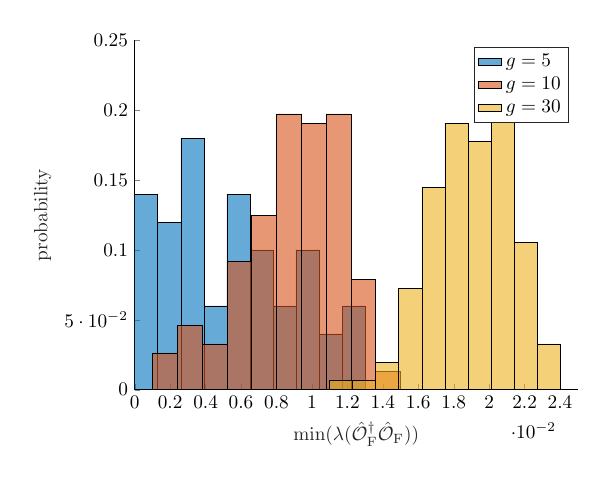
\begin{tikzpicture}[thick,scale=0.49, every node/.style={scale=1.42}]

\begin{axis}[%
width=4.521in,
height=3.566in,
at={(0.758in,0.481in)},
scale only axis,
xmin=0,
xmax=0.025,
xlabel style={font=\color{white!15!black}},
xlabel={${\rm min}(\lambda(\hat{\mathcal{O}}_{\rm F}^\dagger \hat{\mathcal{O}}_{\rm F}))$},
ymin=0,
ymax=0.25,
ylabel style={font=\color{white!15!black}},
ylabel={probability},
axis background/.style={fill=white},
axis x line*=bottom,
axis y line*=left,
legend style={legend cell align=left, align=left, draw=white!15!black}
]
\addplot[ybar interval, fill=mycolor1, fill opacity=0.6, draw=black, area legend] table[row sep=crcr] {%
x	y\\
0	0.14\\
0.0013	0.12\\
0.0026	0.18\\
0.0039	0.06\\
0.0052	0.14\\
0.0065	0.1\\
0.0078	0.06\\
0.0091	0.1\\
0.0104	0.04\\
0.0117	0.06\\
0.013	0.06\\
};
\addlegendentry{$g = 5$}

\addplot[ybar interval, fill=mycolor2, fill opacity=0.6, draw=black, area legend] table[row sep=crcr] {%
x	y\\
0.001	0.0263157894736842\\
0.0024	0.0460526315789474\\
0.0038	0.0328947368421053\\
0.0052	0.0921052631578947\\
0.0066	0.125\\
0.008	0.197368421052632\\
0.0094	0.190789473684211\\
0.0108	0.197368421052632\\
0.0122	0.0789473684210526\\
0.0136	0.0131578947368421\\
0.015	0.0131578947368421\\
};
\addlegendentry{$g = 10$}

\addplot[ybar interval, fill=mycolor3, fill opacity=0.6, draw=black, area legend] table[row sep=crcr] {%
x	y\\
0.011	0.00657894736842105\\
0.0123	0.00657894736842105\\
0.0136	0.0197368421052632\\
0.0149	0.0723684210526316\\
0.0162	0.144736842105263\\
0.0175	0.190789473684211\\
0.0188	0.177631578947368\\
0.0201	0.243421052631579\\
0.0214	0.105263157894737\\
0.0227	0.0328947368421053\\
0.024	0.0328947368421053\\
};
\addlegendentry{$g = 30$}

\end{axis}
\end{tikzpicture}%
\hspace{0.2cm}
% This file was created by matlab2tikz.
%
%The latest updates can be retrieved from
%  http://www.mathworks.com/matlabcentral/fileexchange/22022-matlab2tikz-matlab2tikz
%where you can also make suggestions and rate matlab2tikz.
%
\definecolor{mycolor1}{rgb}{0.00000,0.44700,0.74100}%
\definecolor{mycolor2}{rgb}{0.85000,0.32500,0.09800}%
\definecolor{mycolor3}{rgb}{0.92900,0.69400,0.12500}%
%
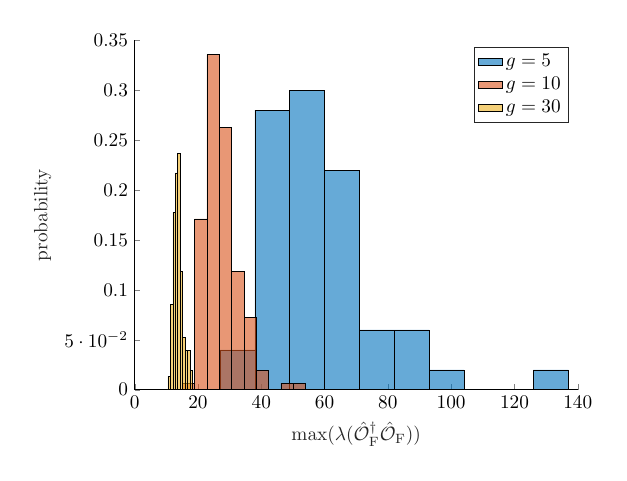
\begin{tikzpicture}[thick,scale=0.49, every node/.style={scale=1.42}]

\begin{axis}[%
width=4.521in,
height=3.566in,
at={(0.758in,0.481in)},
scale only axis,
xmin=0,
xmax=140,
xlabel style={font=\color{white!15!black}},
xlabel={${\rm max}(\lambda(\hat{\mathcal{O}}_{\rm F}^\dagger \hat{\mathcal{O}}_{\rm F}))$},
ymin=0,
ymax=0.35,
ylabel style={font=\color{white!15!black}},
ylabel={probability},
axis background/.style={fill=white},
axis x line*=bottom,
axis y line*=left,
legend style={legend cell align=left, align=left, draw=white!15!black}
]
\addplot[ybar interval, fill=mycolor1, fill opacity=0.6, draw=black, area legend] table[row sep=crcr] {%
x	y\\
27	0.04\\
38	0.28\\
49	0.3\\
60	0.22\\
71	0.06\\
82	0.06\\
93	0.02\\
104	0\\
115	0\\
126	0.02\\
137	0.02\\
};
\addlegendentry{$g = 5$}

\addplot[ybar interval, fill=mycolor2, fill opacity=0.6, draw=black, area legend] table[row sep=crcr] {%
x	y\\
15	0.00657894736842105\\
18.9	0.171052631578947\\
22.8	0.335526315789474\\
26.7	0.263157894736842\\
30.6	0.118421052631579\\
34.5	0.0723684210526316\\
38.4	0.0197368421052632\\
42.3	0\\
46.2	0.00657894736842105\\
50.1	0.00657894736842105\\
54	0.00657894736842105\\
};
\addlegendentry{$g = 10$}

\addplot[ybar interval, fill=mycolor3, fill opacity=0.6, draw=black, area legend] table[row sep=crcr] {%
x	y\\
10.5	0.0131578947368421\\
11.27	0.0855263157894737\\
12.04	0.177631578947368\\
12.81	0.217105263157895\\
13.58	0.236842105263158\\
14.35	0.118421052631579\\
15.12	0.0526315789473684\\
15.89	0.0394736842105263\\
16.66	0.0394736842105263\\
17.43	0.0197368421052632\\
18.2	0.0197368421052632\\
};
\addlegendentry{$g = 30$}

\end{axis}
\end{tikzpicture}%
\caption{Histogram plot of the distribution of the minimal and maximal eigenvalue of the operator $\hat{\mathcal{O}}_{\rm F}\hat{\mathcal{O}}_{\rm F}^{\dagger}$ for one replicum with 400 field configurations for $L=12$ and $g=5,10,30$. For high values of $g$ the smallest eigenvalues are clearly separated from zero which ensures the stability of the simulation. With decreasing $g$ the smallest eigenvalues come arbitrarily close to zero whereas the largest eigenvalues increase at the same time which leads to high condition numbers of the fermionic operator and threatens the stability of the simulation. \label{fig: ev_dist}}
\end{figure}
%

Additional simulations have been conducted for fixed $LM=6$ to check for the influence of finite volume effects and with $r=0$ which means without the presence of a \names{Wilson} term to check its influence on the observables.\\
We can observe that for lower $g$ values the simulations become more involved. For too small values of $g$ the conjugate gradient method to solve (\ref{eq: mscg}) does not converge. This is due to the eigenvalue spectrum of the fermion matrix $\hat{\mathcal{O}}_{\rm F}$ shown in \autoref{fig: ev_dist}. For small $g$ the condition number of $\hat{\mathcal{O}}_{\rm F}$ (which is basically the ratio of the largest and smallest eigenvalue) becomes very bad. The smallest eigenvalues are so close to zero that they might leave the regime of accuracy of the rational approximation (\ref{eq: rat_approx}) and are within the range of errors of the conjugate gradient solver which could cause a phase transition of the \names{Pfaffian}. During our simulation with $LM=4$ and a present \names{Wilson} term this behaviour occurred for the first time for $g=5$ . We tried to cure this peculiarity with help of a reweighting procedure which was introduced first in \cite{Ferrenberg:1988yz} (see also \cite{Luscher:2008tw,Finkenrath:2013soa}). Therefore we add a twisted mass term to the fermionic matrix to obtain
%
%
\begin{align}
\tilde{\mathcal{O}}_{\rm F} &= \hat{\mathcal{O}}_{\rm F} + i\mu \Gamma_{5},  &
\tilde{\mathcal{O}}_{\rm F} \tilde{\mathcal{O}}_{\rm F}^{\dagger} &= \hat{\mathcal{O}}_{\rm F}\hat{\mathcal{O}}_{\rm F}^{\dagger} + \mu^{2}\mathds{1},
\end{align}
%
%
where $\mu$ is the reweighting mass parameter. The term $\mu^{2}\mathds{1}$ will shift the eigenvalues of $\tilde{\mathcal{O}}_{\rm F} \tilde{\mathcal{O}}_{\rm F}^{\dagger}$ apart from zero and ensures the stability of the simulation. Hereby the crucial term in measuring an observable is the \names{Pfaffian} which is included in the probability distribution in the RHMC. We want to estimate observables generated from a distribution without an additional mass term by actually doing simulations with a twisted mass. While assuming the \names{Pfaffian} to be positive we can write
%
%
\begin{equation}
\begin{alignedat}{2}
\pf\big(\hat{\mathcal{O}}_{\rm F}\big) &= \left(\frac{\det \big(\hat{\mathcal{O}}_{\rm F} \hat{\mathcal{O}}_{\rm F}^{\dagger} \big)}{\det \big(\tilde{\mathcal{O}}_{\rm F} \tilde{\mathcal{O}}_{\rm F}^{\dagger} \big)}\right)^{\frac{1}{4}} \pf\big(\tilde{\mathcal{O}}_{\rm F}\big)\\
%
&\equiv W \;\pf\left(\tilde{\mathcal{O}}_{\rm F}\right).
\end{alignedat}
\label{eq: rew_factor}
\end{equation}
%
%
For a small reweighting mass $\mu$ we can thus compute an estimate of the observable vev without the twisted mass $\langle O \rangle_{0}$ via
%
%
\begin{equation}
\langle O \rangle_{0} = \frac{\langle O W \rangle_{\mu}}{\langle W \rangle_{\mu}} .
\end{equation}
%
%
The vev $\langle O \rangle_{\mu}$ represents the value obtained from a RHMC simulation with twisted mass term and $W$ is the reweighting factor defined in (\ref{eq: rew_factor}). It can be expressed in terms of $\;\widetilde{\!W}=W^{4}$ which can be rewritten to
%
%
\begin{equation}
\widetilde{\!W} = \frac{\det \left(\hat{\mathcal{O}}_{\rm F}\hat{\mathcal{O}}_{\rm F}^{\dagger}\right)}{\det\left(\hat{\mathcal{O}}_{\rm F}\hat{\mathcal{O}}_{\rm F}^{\dagger}+ \mu^{2}\right)} = \frac{1}{\det\left( \mathds{1}+\frac{\mu^{2}}{\hat{\mathcal{O}}_{\rm F}\hat{\mathcal{O}}_{\rm F}^{\dagger}}\right)} \equiv \frac{1}{\det M}.
\end{equation}
%
%
In a separate MC integration we estimate $\;\widetilde{\!W}$ by using
%
%
\begin{equation}
\frac{1}{\det M} = \int \mathcal{D}\xi \; e^{-\xi^{\dagger}M\xi} = \int \mathcal{D}\xi\; \left(\frac{e^{-\xi^{\dagger}M\xi}}{\rho(\xi)}\right) \rho(\xi),
\end{equation}
%
%
where the complex fields $\xi$ are distributed according to $\rho(\xi)$ so that by (\ref{eq: vev_rho}) we can write
%
%
\begin{equation}
\frac{1}{\det M} = \left\langle \frac{e^{-\xi^{\dagger}M\xi}}{\rho(\xi)}\right\rangle_{\rho}.
\end{equation}
%
%
With a \names{Gaussian} distribution $\rho(\xi)=\exp(-\xi^{\dagger}\xi)$ we find the stochastic estimation
%
%
\begin{equation}
\begin{alignedat}{2}
\widetilde{\!W} &= \left\langle \exp \left[ -\xi^{\dagger}\left(\frac{\mu^{2}}{\hat{\mathcal{O}}_{\rm F}\hat{\mathcal{O}}_{\rm F}^{\dagger}}\right)\xi\right]\right\rangle_{\rho} \\
&= \frac{1}{N_{\xi}} \sum\limits_{k=1}^{N_{\xi}} \exp \left[ -\xi_{k}^{\dagger}\left(\frac{\mu^{2}}{\hat{\mathcal{O}}_{\rm F}\hat{\mathcal{O}}_{\rm F}^{\dagger}}\right)\xi_{k}\right] + \mathcal{O}\left(\frac{1}{\sqrt{N_{\xi}}}\right). 
\end{alignedat}
\end{equation}
%
%
The reweighting procedure is of course also limited in its application and is only valid for small shifts $\mu$. We therefore choose $\mu$ as small a possible, but large enough to ensure the stability of the simulation. Reweighting has only been applied for the collection of data with $g=5$. A plot of the reweighting factors for a collection of field configurations is given in \autoref{fig: rew_factor}.
%
%
\begin{figure}
\centering
% This file was created by matlab2tikz.
%
%The latest updates can be retrieved from
%  http://www.mathworks.com/matlabcentral/fileexchange/22022-matlab2tikz-matlab2tikz
%where you can also make suggestions and rate matlab2tikz.
%
\definecolor{mycolor1}{rgb}{0.00000,0.44700,0.74100}%
%
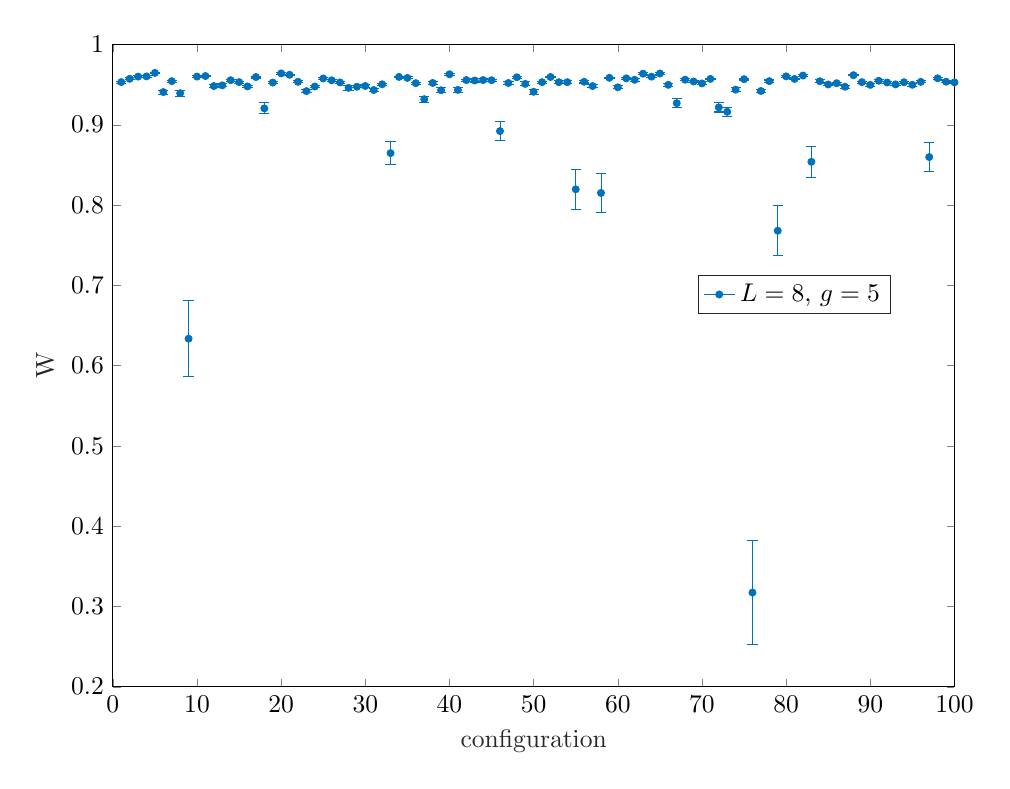
\begin{tikzpicture}[thick,scale=0.65, every node/.style={scale=1.42}]

\begin{axis}[%
width=6.474in,
height=4.941in,
at={(1.086in,0.667in)},
scale only axis,
xmin=0,
xmax=100,
xlabel style={font=\color{white!15!black}},
xlabel={configuration},
ymin=0.2,
ymax=1,
ylabel style={font=\color{white!15!black}},
ylabel={W},
axis background/.style={fill=white},
legend style={at={(0.695,0.580)}, anchor=south west, legend cell align=left, align=left, draw=white!15!black}
]
\addplot [color=mycolor1, draw=none, mark=*, mark options={solid, mycolor1}]
 plot [error bars/.cd, y dir = both, y explicit]
 table[row sep=crcr, y error plus index=2, y error minus index=3]{%
1	0.953030237078629	0.00133252750175868	0.00133252750175868\\
2	0.957150503958378	0.00119541958365667	0.00119541958365667\\
3	0.959889343761428	0.000938639147507316	0.000938639147507316\\
4	0.960154724973424	0.000980984469972055	0.000980984469972055\\
5	0.964550865872029	0.000885901666303172	0.000885901666303172\\
6	0.940630342232228	0.00250014555798991	0.00250014555798991\\
7	0.95425368547006	0.00134627394156228	0.00134627394156228\\
8	0.939178886966104	0.00364762466007334	0.00364762466007334\\
9	0.633457123731367	0.0472812228023222	0.0472812228023222\\
10	0.959909327569502	0.00103165385055101	0.00103165385055101\\
11	0.960636529655091	0.000993794898290946	0.000993794898290946\\
12	0.948113096374446	0.00164624057217347	0.00164624057217347\\
13	0.948987707828379	0.00176526783317368	0.00176526783317368\\
14	0.955407054926832	0.00102583085103299	0.00102583085103299\\
15	0.95301757863849	0.00132418935991981	0.00132418935991981\\
16	0.947679854894374	0.00153199275427202	0.00153199275427202\\
17	0.959352875272271	0.00119627867197684	0.00119627867197684\\
18	0.92033007845509	0.00682364997758111	0.00682364997758111\\
19	0.952508277360915	0.00172500091360881	0.00172500091360881\\
20	0.963873665091126	0.00103646762309367	0.00103646762309367\\
21	0.962157023803847	0.000927329331847737	0.000927329331847737\\
22	0.953414705142051	0.00120583910539539	0.00120583910539539\\
23	0.941811545902577	0.00202128776547507	0.00202128776547507\\
24	0.947558482395904	0.00158327009637249	0.00158327009637249\\
25	0.957605784753993	0.00106264386370841	0.00106264386370841\\
26	0.955273845405733	0.00123305917534755	0.00123305917534755\\
27	0.952639377407374	0.00126588986455126	0.00126588986455126\\
28	0.945883790489921	0.00282828561486714	0.00282828561486714\\
29	0.947256171198881	0.00144419082841063	0.00144419082841063\\
30	0.94820267448161	0.00176587703858765	0.00176587703858765\\
31	0.943184661822536	0.00200102907947995	0.00200102907947995\\
32	0.95030527660898	0.00135555392329708	0.00135555392329708\\
33	0.864600630067417	0.0138665801521919	0.0138665801521919\\
34	0.959494596516065	0.00106178032940392	0.00106178032940392\\
35	0.958262203839964	0.00117518759982681	0.00117518759982681\\
36	0.951728637235856	0.00134118468783136	0.00134118468783136\\
37	0.931780729524544	0.00389548704409748	0.00389548704409748\\
38	0.951969281285472	0.0015905678557486	0.0015905678557486\\
39	0.942897397932175	0.00288314367089374	0.00288314367089374\\
40	0.962801959652657	0.000942267336577612	0.000942267336577612\\
41	0.943341501353021	0.00299144713265679	0.00299144713265679\\
42	0.955590102423167	0.00126290870156753	0.00126290870156753\\
43	0.955029871693714	0.00199665335475273	0.00199665335475273\\
44	0.955596016646912	0.00196009278229093	0.00196009278229093\\
45	0.95538322164712	0.00120800088016777	0.00120800088016777\\
46	0.892045291014329	0.0115879692227173	0.0115879692227173\\
47	0.951930834426785	0.00146421466764669	0.00146421466764669\\
48	0.959088952324944	0.00106624518326287	0.00106624518326287\\
49	0.950817778162411	0.00250484836843084	0.00250484836843084\\
50	0.94098199387842	0.00314342094419687	0.00314342094419687\\
51	0.952975676672323	0.00117230657139859	0.00117230657139859\\
52	0.959437566623347	0.00114593847921524	0.00114593847921524\\
53	0.9529353653296	0.00165806316688042	0.00165806316688042\\
54	0.952950831077942	0.00162301354293535	0.00162301354293535\\
55	0.819554846129553	0.0247535548286678	0.0247535548286678\\
56	0.953440624254973	0.00149219885353142	0.00149219885353142\\
57	0.948141519838406	0.0019286852994215	0.0019286852994215\\
58	0.814992678051219	0.0245005448875132	0.0245005448875132\\
59	0.958393894530529	0.00097280326016195	0.00097280326016195\\
60	0.946546721388823	0.00182834210760782	0.00182834210760782\\
61	0.957732765305165	0.00117635994842812	0.00117635994842812\\
62	0.955937182771325	0.00171349766823078	0.00171349766823078\\
63	0.963538091033205	0.000940623779681627	0.000940623779681627\\
64	0.95983422439546	0.0010161829723555	0.0010161829723555\\
65	0.963804252331302	0.000883008611638947	0.000883008611638947\\
66	0.94962616802567	0.00149509917142102	0.00149509917142102\\
67	0.926821623991233	0.00535990810269077	0.00535990810269077\\
68	0.95605174092749	0.00115661048423661	0.00115661048423661\\
69	0.953794711664734	0.0012541138672125	0.0012541138672125\\
70	0.951400907443644	0.0018416549464992	0.0018416549464992\\
71	0.957042285437107	0.00110050577073512	0.00110050577073512\\
72	0.921512874925344	0.00569830331322003	0.00569830331322003\\
73	0.916099596153376	0.00564391378234099	0.00564391378234099\\
74	0.943635049120853	0.0021690054878531	0.0021690054878531\\
75	0.956696127635527	0.00102188357832909	0.00102188357832909\\
76	0.317304067216777	0.0650047425101933	0.0650047425101933\\
77	0.94195289707923	0.00217745247239805	0.00217745247239805\\
78	0.954234643325438	0.00145101213854869	0.00145101213854869\\
79	0.76791689295441	0.0311627009032048	0.0311627009032048\\
80	0.96017928087135	0.000912753749224784	0.000912753749224784\\
81	0.956987293675572	0.00108595177225456	0.00108595177225456\\
82	0.961234216875208	0.000974614169321383	0.000974614169321383\\
83	0.8537657003846	0.0196867456405926	0.0196867456405926\\
84	0.954119061308469	0.00187684099599671	0.00187684099599671\\
85	0.950098018044003	0.00170348621936121	0.00170348621936121\\
86	0.9516707643426	0.00131003428950105	0.00131003428950105\\
87	0.947278846969526	0.0018195681291547	0.0018195681291547\\
88	0.961655888062194	0.000913532793973008	0.000913532793973008\\
89	0.952978002586837	0.00123933068894702	0.00123933068894702\\
90	0.949582524031137	0.00166419626807651	0.00166419626807651\\
91	0.954651874137725	0.00120076736459215	0.00120076736459215\\
92	0.952537415324764	0.00178893006311692	0.00178893006311692\\
93	0.95018692827487	0.00153026371929073	0.00153026371929073\\
94	0.952850106052462	0.00123685441470036	0.00123685441470036\\
95	0.949711065577833	0.00154142732689481	0.00154142732689481\\
96	0.953372142400315	0.00135941003584396	0.00135941003584396\\
97	0.859707568991088	0.0176151461723741	0.0176151461723741\\
98	0.957796286548261	0.00102062929286917	0.00102062929286917\\
99	0.953529010681909	0.00119134339575414	0.00119134339575414\\
100	0.952725852303406	0.00107041036437602	0.00107041036437602\\
};
\addlegendentry{$L=8$, $g=5$}

\end{axis}
\end{tikzpicture}%
\caption{The reweighting factor $W$ for a collection of 100 field configurations for $L=8$ and $g=5$. Most values are very close to one , pointing out a good estimate in this region, but there are also a few much lower values that might indicate a transition of the \names{Pfaffian} phase and therefore a too small $\mu$. \label{fig: rew_factor}}
\end{figure}
%
%
%
%
%
%
% - - - - - - - - - -    Observables   - - - - - - - - - - 
%
%
%
%
%
\section{Observables}
As pointed out earlier we are utmost interested in obtaining information on the scaling function $f(g)$. In our numerical simulation we are basically restricted to calculate observable vevs and therefore need to find a suitable observable providing a connection to $f(g)$. By recapitulating (\ref{eq: W_S_cusp}) we can write
%
%
\begin{equation}
-\ln Z_{\rm cusp} = \frac{1}{8} f(g)V_{2}.
\end{equation}
%
%
With $Z_{\rm cusp} = \int \mathcal{D}\delta X\,\mathcal{D}\delta \mathit{\Psi}\;e^{-S_{\rm cusp}}$ and the structure of the action 
\begin{equation}
S_{\rm cusp} = g \int \dd t \dd s \; \mathcal{L}_{\rm cusp}
\end{equation}
we find
%
%
\begin{equation}
\langle S_{\rm cusp} \rangle = \frac{\int \mathcal{D}\delta X\,\mathcal{D}\delta\mathit{\Psi} \; S_{\rm cusp} \;e^{-S_{\rm cusp}}}{\int \mathcal{D}\delta X\,\mathcal{D}\delta\mathit{\Psi} \; e^{-S_{\rm cusp}}} = -g \frac{\dd \ln Z_{\rm cusp}}{\dd g} \equiv g\frac{V_{2}}{2} f'(g).
\label{eq: <S_cusp>}
\end{equation}
%
%
We can therefore obtain information on the derivative of the scaling function from the vev of the action.\\
To motivate our line of constant physics, we investigate the mass of the bosonic fluctuation field $x$ around the string vacuum which can be obtained from the correlation function $\langle x x^{*}\rangle$.
%
%
%
%
%  - - - - - -   < x x* >  - - - - - - - -
%
%
%
% 
\subsection[The $\langle xx^{*}\rangle$ correlator]{The {$\mathitbf{\langle x\,x^{*}\rangle}$} correlator} \label{sec: xx_corr}
We define the physical masses of the $x,x^{*}$ fields as the values of the energy at vanishing momentum. In the large coupling limit the mass can be read off from a quadratic expansion of the \names{Lagrangian} \cite{Bianchi:2016cyv} to 
%
%
\begin{equation}
\frac{m_{x}^{2}}{m^{2}} \quad \textabove{=}{$\small g \!\gg \!1$} \quad \frac{1}{2}.
\end{equation}
%
%
The leading quantum corrections to the dispersion limit of the regarding fields have been computed in \cite{Giombi:2010bj}, leading to (\ref{eq: m_x}). We can determine the mass for different values of the coupling to estimate a dependence of $m_{x}^{2}$ of $g$. For a fixed value of $g$ one can calculate the physical mass on the lattice with timeslice correlation functions derived from the connected two-point functions
%
%
\begin{equation}
G_{x}(t_{1},s_{1};t_{2},s_{2}) = \langle x(t_{1},s_{1})\, x^{*}(t_{2},s_{2}) \rangle_{\rm c},
\end{equation}
%
%
which coincide with the regular two-point functions in the case of a present $SO(2)$ symmetry. A \names{Fourier} transform in the spatial components results in the \textit{timeslice correlator}
%
%
\begin{equation}
C_{x}(t,k) = \frac{1}{L}\sum\limits_{s_{1},s_{2}} e^{-ik(s_{1}-s_{2})} G_{x}(t,s_{1};0,s_{2}).
\end{equation}
%
%
Thinking in terms of particle eigenstates $\vert k \rangle = \vert k,\alpha \rangle$, where $k$ corresponds to the spatial momentum and $\alpha$ to different energy states, one would find for a momentum and energy operator $P$ and $H$
%
%
\begin{align}
P \vert k,\alpha \rangle &= k \vert k,\alpha \rangle, \\
H \vert k,\alpha \rangle &= E(k,\alpha) \vert k,\alpha \rangle.
\end{align}
%
%
We can therefore think in general of $C(t,k)$ representing (see \cite{montvay_lattice})
%
%
\begin{equation}
C(t,k) = \langle k\vert e^{-tH} \vert k \rangle = \sum\limits_{\alpha} \vert c_{\alpha} \vert^{2} e^{-t E(k,\alpha)}.
\raisetag{-8pt}
\end{equation}
%\hfill
%\vspace{0.2cm}
%
%
For large $t$ the lowest energy $E(k,0)$ dominates the timeslice correlator. It can be recognised as the energy of a one-particle state and we can identify a physical mass with the energy at vanishing momentum
%
%
\begin{equation}
m \equiv E(0,0).
\end{equation}
%
%
For the $x$ fields we can therefore make the same assumptions and identify
%
%
\begin{equation}
C_{x}(t) \equiv C_{x}(t,0) \quad \textabove{\sim}{$\footnotesize t\!\gg\!1$} \quad e^{-tm_{x \rm LAT}}, \qquad m_{x\rm LAT} = E_{x}(k=0).
\end{equation}
%
%
The temporal boundary conditions on the lattice require to respect also a left moving part, since
%
%
\begin{equation}
C_{x}(t) = C_{x}(T-t)
\end{equation}
%
%
and thus
%
%
\begin{equation}
C_{x}(t) \quad \textabove{\sim}{$\footnotesize t\!\gg\!1$} \quad e^{-tm_{x \rm LAT}}+e^{-(T-t)m_{x \rm LAT}} \sim \text{cosh\,}\left(\left(\frac{T}{2}-t\right) m_{x\rm LAT}\right).
\end{equation}
%
%
%
%
On the lattice we can determine $m_{x\rm LAT}$ as a limit of an \textit{effective mass} $m_{x}^{\rm eff}$. For fixed values of $g$ and $T$ we can estimate $m_{x}^{\rm eff}(g,T)$ by a fit of the timeslice correlator $C_{x}(t)$ to the curve (see \autoref{fig: coshcorr})
%
%
\begin{equation}
A\cdot e^{-Tm_{x}^{\rm eff}/2}\cdot\text{cosh\,}\left(\left(\frac{T}{2}-t\right) m_{x}^{\rm eff}\right)
\label{eq: cosh_fit}
\end{equation}
%
%
in a regime of $t$ close to $T/2$ where excited states are suppressed. To obtain the continuum value, we extrapolate $m_{x}^{\rm eff}(g,T)$ for different lattice sizes (see \autoref{fig: massfit_cosh}) to find
%
%
\begin{equation}
m_{x\rm LAT}(g) = \lim\limits_{T\to \infty} m_{x}^{\rm eff}(g,T).
\end{equation}
To improve the fit that estimates $m_{x}^{\rm eff}$ we chose the temporal lattice extent to be twice the spatial one. There is in fact another issue we need to consider. A present \names{Wilson} term breaks the $SO(2)$ symmetry and the connected correlators do not coincide with the disconnected ones. With the spatially \names{Fourier} transformed fields at zero momentum
%
%
\begin{equation}
\tilde{x}(t)\equiv\frac{1}{\sqrt{L}} \sum\limits_{s} x(t,s)
\end{equation}
%
%
we can rewrite the timeslice correlators in the following way
%
%
\begin{equation}
C_{x}(t) = \langle \tilde{x}(t) \tilde{x}^{*}(0) \rangle_{\rm c},
\end{equation}
%
%
where the connected correlator is defined as
%
%
\begin{equation}
\langle \tilde{x}(t) \tilde{x}^{*}(0) \rangle_{\rm c} \equiv \langle \tilde{x}(t) \tilde{x}^{*}(0) \rangle - \langle \tilde{x}\rangle \langle \tilde{x}^{*}\rangle
\end{equation}
%
%
In the lattice simulation we implement the $x$ field as its real and imaginary part $x_{\rm R}$ and $x_{\rm I}$ and thus want to write the correlator in terms of these components
%
%
\begin{equation}
\begin{alignedat}{2}
\langle \tilde{x}(t) \tilde{x}^{*}(0) \rangle_{\rm c} &= \langle\tilde{x}_{\rm R}(t)\tilde{x}_{\rm R}(0)\rangle + \langle \tilde{x}_{\rm I}(t)\tilde{x}_{\rm I}(0)\rangle \\
&\quad +i \left( \langle\tilde{x}_{\rm I}(t)\tilde{x}_{\rm R}(0)\rangle - \langle\tilde{x}_{\rm R}(t)\tilde{x}_{\rm I}(0)\rangle \right) \\
&\quad - \langle \tilde{x}_{\rm R}\rangle^{2} - \langle \tilde{x}_{\rm I}\rangle^{2}.
\end{alignedat}
\end{equation}
%
%
The second line will vanish according to translational invariance and time reversal. We can thus calculate the connected timeslice correlators as
%
%
\begin{equation}
C_{x}(t) = \langle\tilde{x}_{\rm R}(t)\tilde{x}_{\rm R}(0)\rangle + \langle \tilde{x}_{\rm I}(t)\tilde{x}_{\rm I}(0)\rangle - \langle \tilde{x}_{\rm R}\rangle^{2} - \langle \tilde{x}_{\rm I}\rangle^{2}.
\end{equation}
%
%
%
Numerically we checked the two conditions
\begin{equation}
\begin{alignedat}{2}
\langle \tilde{x}_{k}(t)\, \tilde{x}_{i}(0)\rangle &= 0 \quad k\neq i, \; k,i\in \lbrace {\rm R,I}, \\
\langle \tilde{x}_{\rm R}\rangle &= - \langle \tilde{x}_{\rm I}\rangle.
\end{alignedat}
\end{equation}
%
%
%
Applying these we can calculate the connected timeslice correlator via
%
%
\begin{equation}
C_{x}(t) = \langle\tilde{x}_{\rm R}(t)\tilde{x}_{\rm R}(0) + \tilde{x}_{\rm I}(t)\tilde{x}_{\rm I}(0) + \tilde{x}_{\rm R}(t)\tilde{x}_{\rm I}(0) + \tilde{x}_{\rm I}(t)\tilde{x}_{\rm R}(0) \rangle.
\label{eq: conn_corr}
\end{equation}
%
%
%
We want to emphasise here that we can subtract the non-connected part for every configuration and then do the average. This reduces the statistical errors compared to the previous method.
%
%
%
\begin{figure}
\centering
% This file was created by matlab2tikz.
%
%The latest updates can be retrieved from
%  http://www.mathworks.com/matlabcentral/fileexchange/22022-matlab2tikz-matlab2tikz
%where you can also make suggestions and rate matlab2tikz.
%
\begin{tikzpicture}[thick,scale=0.9, every node/.style={scale=0.9}]

\begin{axis}[%
width=4.585in,
height=3.591in,
at={(0.769in,0.485in)},
scale only axis,
xmin=-1,
xmax=24,
xlabel style={font=\color{white!15!black}},
xlabel={$t/a$},
ymin=0,
ymax=0.025,
ylabel style={font=\color{white!15!black}},
ylabel={$C_x(at)$},
axis background/.style={fill=white},
axis x line*=bottom,
axis y line*=left,
legend style={legend cell align=left, align=left, draw=white!15!black}
]
\addplot [color=blue, draw=none, mark size=1.0pt, mark=*, mark options={solid, fill=blue, blue}]
 plot [error bars/.cd, y dir = both, y explicit]
 table[row sep=crcr, y error plus index=2, y error minus index=3]{%
0	0.0243260688956114	0.000508141001299536	0.000508141001299536\\
1	0.0190365611462439	0.000495256840816025	0.000495256840816025\\
2	0.0151613082921611	0.00047550688870233	0.00047550688870233\\
3	0.0120268515516549	0.000452641748717815	0.000452641748717815\\
4	0.00954649117718522	0.000437780862197653	0.000437780862197653\\
5	0.00799378320884425	0.000427874857138029	0.000427874857138029\\
6	0.00664231426579697	0.000424177616634774	0.000424177616634774\\
7	0.00570072604922918	0.000432623989008807	0.000432623989008807\\
8	0.00468960623594428	0.000438472127189161	0.000438472127189161\\
9	0.00419824652026065	0.000448589313853651	0.000448589313853651\\
10	0.00381004107536998	0.000457257954665896	0.000457257954665896\\
11	0.00331400881610101	0.000476295971796519	0.000476295971796519\\
12	0.00326691499004617	0.000486384238136538	0.000486384238136538\\
13	0.00331400881610101	0.000476295971796519	0.000476295971796519\\
14	0.00381004107536998	0.000457257954665896	0.000457257954665896\\
15	0.00419824652026065	0.000448589313853651	0.000448589313853651\\
16	0.00468960623594429	0.000438472127189161	0.000438472127189161\\
17	0.00570072604922918	0.000432623989008807	0.000432623989008807\\
18	0.00664231426579697	0.000424177616634774	0.000424177616634774\\
19	0.00799378320884425	0.000427874857138029	0.000427874857138029\\
20	0.00954649117718522	0.000437780862197653	0.000437780862197653\\
21	0.0120268515516549	0.000452641748717815	0.000452641748717815\\
22	0.0151613082921611	0.00047550688870233	0.00047550688870233\\
23	0.0190365611462439	0.000495256840816025	0.000495256840816025\\
};
\addlegendentry{Data: $L=12$ $g=100$}

\addplot [color=red]
  table[row sep=crcr]{%
1	0.018815021481251\\
2	0.015153649523578\\
3	0.0122333397946224\\
4	0.00991127975058608\\
5	0.00807391318253274\\
6	0.00663138695232729\\
7	0.00551315688501861\\
8	0.00466453793166128\\
9	0.0040440298944364\\
10	0.00362128793342356\\
11	0.00337563860627392\\
12	0.00329506887034864\\
13	0.00337563860627392\\
14	0.00362128793342356\\
15	0.0040440298944364\\
16	0.00466453793166128\\
17	0.00551315688501861\\
18	0.00663138695232729\\
19	0.00807391318253274\\
20	0.00991127975058608\\
21	0.0122333397946224\\
22	0.015153649523578\\
23	0.018815021481251\\
};
\addlegendentry{Fit to cosh}

\addplot [color=red, dashed]
  table[row sep=crcr]{%
1	0.0185686944823777\\
2	0.0147741284170975\\
3	0.0117793632850322\\
4	0.00942227676804811\\
5	0.0075752674305322\\
6	0.00613834698552117\\
7	0.00503372740515777\\
8	0.00420160984742034\\
9	0.00359694743167847\\
10	0.0031870066151649\\
11	0.0029495951549023\\
12	0.00287186072538535\\
13	0.0029495951549023\\
14	0.0031870066151649\\
15	0.00359694743167847\\
16	0.00420160984742034\\
17	0.00503372740515777\\
18	0.00613834698552117\\
19	0.0075752674305322\\
20	0.00942227676804811\\
21	0.0117793632850322\\
22	0.0147741284170975\\
23	0.0185686944823777\\
};
\addlegendentry{Fit errors}

\addplot [color=red, dashed, forget plot]
  table[row sep=crcr]{%
1	0.0190739501095884\\
2	0.0155526061974642\\
3	0.0127146450612897\\
4	0.0104353664588898\\
5	0.00861461870387236\\
6	0.00717239799241623\\
7	0.00604533302965205\\
8	0.005183900489833\\
9	0.00455024895739046\\
10	0.00411653573266837\\
11	0.00386370342144523\\
12	0.00378064255148857\\
13	0.00386370342144523\\
14	0.00411653573266837\\
15	0.00455024895739046\\
16	0.005183900489833\\
17	0.00604533302965205\\
18	0.00717239799241623\\
19	0.00861461870387236\\
20	0.0104353664588898\\
21	0.0127146450612897\\
22	0.0155526061974642\\
23	0.0190739501095884\\
};
\end{axis}
\end{tikzpicture}%
\caption{Plot of the timeslice correlator $C_{x}(t)$ for a measurement of 400 field configurations with $L=12$ and $g=100$ without a \names{Wilson} term (blue dots). The parameters $A$ and $m_{x}^{\rm eff}$ have been determined by a fit and the corresponding curve (\ref{eq: cosh_fit}) is given in red with the errors of the effective mass as dashed lines.\label{fig: coshcorr}}
\end{figure}
%
%
\begin{figure}
\centering
% This file was created by matlab2tikz.
%
%The latest updates can be retrieved from
%  http://www.mathworks.com/matlabcentral/fileexchange/22022-matlab2tikz-matlab2tikz
%where you can also make suggestions and rate matlab2tikz.
%
\definecolor{mycolor1}{rgb}{0.00000,0.44700,0.74100}%
%
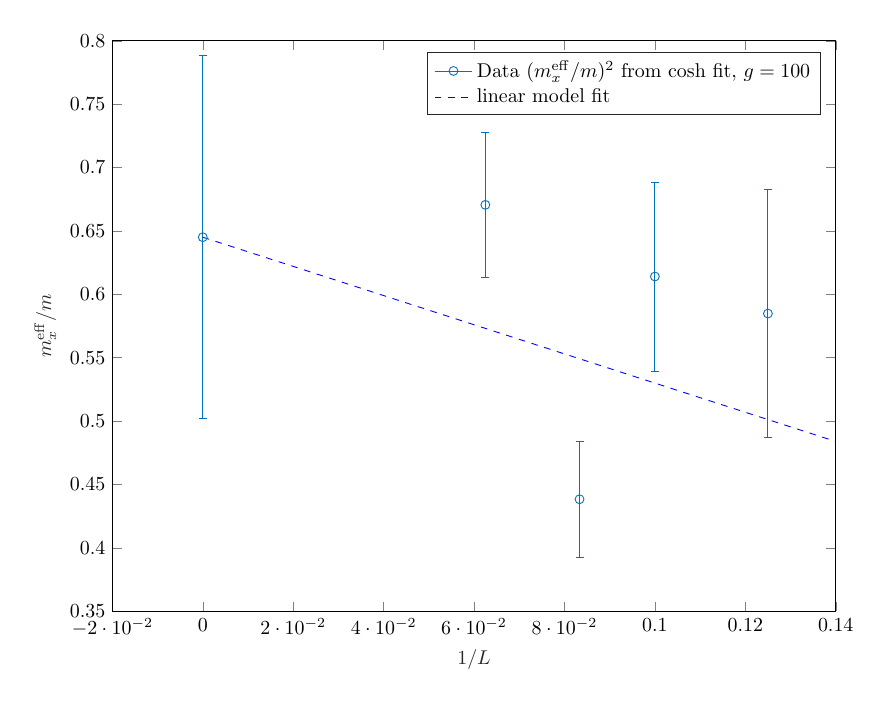
\begin{tikzpicture}[thick,scale=0.8, every node/.style={scale=0.9}]

\begin{axis}[%
width=4.521in,
height=3.566in,
at={(0.758in,0.481in)},
scale only axis,
xmin=-0.02,
xmax=0.14,
xlabel style={font=\color{white!15!black}},
xlabel={$1/L$},
ymin=0.35,
ymax=0.8,
ylabel style={font=\color{white!15!black}},
ylabel={$m_{x}^{\rm eff}/m$},
axis background/.style={fill=white},
legend style={legend cell align=left, align=left, draw=white!15!black}
]
\addplot [color=mycolor1, draw=none, mark=o, mark options={solid, mycolor1}]
 plot [error bars/.cd, y dir = both, y explicit]
 table[row sep=crcr, y error plus index=2, y error minus index=3]{%
0.0625	0.670560513952906	0.0573438887395148	0.0573438887395148\\
0.0833333333333333	0.438346924164652	0.0455068910892664	0.0455068910892664\\
0.1	0.614033856468322	0.0745890105507399	0.0745890105507399\\
0.125	0.584820357502446	0.0976223242590754	0.0976223242590754\\
0	0.645033273318665	0.143190331713913	0.143190331713913\\
};
\addlegendentry{Data $(m_x^{\rm eff}/m)^2$ from cosh fit, $g=100$}

\addplot [color=blue, dashed]
  table[row sep=crcr]{%
0	0.645033273318665\\
0.01	0.633528314410353\\
0.02	0.622023355502041\\
0.03	0.610518396593729\\
0.04	0.599013437685417\\
0.05	0.587508478777104\\
0.06	0.576003519868792\\
0.07	0.56449856096048\\
0.08	0.552993602052168\\
0.09	0.541488643143856\\
0.1	0.529983684235544\\
0.11	0.518478725327231\\
0.12	0.506973766418919\\
0.13	0.495468807510607\\
0.14	0.483963848602295\\
};
\addlegendentry{linear model fit}

\end{axis}
\end{tikzpicture}%
\caption{This plot shows a simple example of a continuum extrapolation for $m_{x\rm LAT}$ with $g=100$ in absece of a \names{Wilson} term. Every point represents a value $m_{x}^{\rm eff}(T)$ generated from one replicum with 400 field configurations each. The result of the linear regression is added as a point with errorbars at zero. \label{fig: massfit_cosh}}
\end{figure}
%
%
%
%
%
%  - - - - - - - -    cusp action   - - - - - - - - - -
%
%
%
%
\subsection{The cusp action}
To measure the action (\ref{eq: <S_cusp>}) we first explore the regime of large $g$. With fixed $LM=4$ which we think is large enough to omit finite volume effects we recover, according to (\ref{eq: F_LAT}), the following lattice observable, behaving linear in $g$ and containing a quadratic divergence in $L$ in the continuum limit
%
%
\begin{equation}
\langle S_{\rm LAT} \rangle = S_{0} + \frac{c}{2} \left(2L^{2}\right) + \mathcal{O}(L^{-1}), \qquad g\gg 1.
\label{eq: S_LAT}
\end{equation}
%
%
In the continuum we would find
%
%
\begin{equation}
\langle S_{\rm cusp} \rangle = g \frac{V_{2}}{8}f'(g)  \quad \textabove{=}{$\footnotesize g\!\gg\!1$} \quad \frac{V_{2}}{2}g \equiv S_{0},
\end{equation}
%
%
leading to a possible description of $f'(g)$ given by
%
%
\begin{equation}
\frac{\langle S_{\rm cusp }\rangle}{S_{0}} = \frac{f'(g)}{4}.
\label{eq: Scusp_fprime}
\end{equation}
%
%
For a discretised version nonetheless we have to include the mass scale for the action to be dimensionless with respect to the lattice spacing
%
%
\begin{equation}
S_{0} = \frac{V_{2}}{2} m^{2}g = \frac{1}{2}\left(2L^{2}\right) M^{2} g.
\end{equation}
%
%
Furthermore we recall the behaviour $f(g) = 4g + \text{const.} + \mathcal{O}(g^{-1})$ from (\ref{eq: scaling_fct}) and insert $V_{2}=a^{2}(TL)=a^{2}(2L^{2})$, since we always use $T=2L$. $S_{0}$ is the discretised classical action and its value is fixed in each simulation for given $g$ and $LM$. In (\ref{eq: S_LAT}) we observe a term quadratically divergent in $L$ in the continuum limit. To motivate the appearance of such behaviour let us recall that we calculate the vev of the cusp action via
%
%
\begin{equation}
 \langle S_{\rm cusp} \rangle = -g \frac{\dd \ln Z_{\rm cusp}}{\dd g}.
 \end{equation} 
 %
 %
and focus especially on any contribution to the partition function that is of quadratic order in the bosonic and fermionic fields  $Z_{\rm cusp}^{(2)}=Z_{\rm B}^{(2)}Z_{\rm F}^{(2)}$. For these contributions we can schematically write
 %
 %
\begin{equation}
\begin{alignedat}{2}
Z_{\rm B}^{(2)} &= \int \prod\limits_{n=1}^{N_{\rm B}} \mathcal{D}\phi_{n} \; e^{-g \sum\limits_{i=1}^{N_{\rm B}} \int \dd t \dd s\; \phi_{i} \mathcal{O}_{i} \phi_{i}} \\
%
%
&\textabove{=}{$^{\rm LAT}$} \int \prod\limits_{n=1}^{N_{\rm B}} \left( \prod\limits_{k=1}^{\vert \mathit{\Lambda}\vert} \dd \phi_{n}^{(k)} \right) \; e^{-g \sum\limits_{i=1}^{N_{\rm B}} \phi_{i}^{\rm T}\hat{\mathcal{O}}_{i}\phi_{i}} \\
%
%
&= \prod\limits_{i=1}^{N_{\rm B}} \frac{1}{\sqrt{\det (g \hat{\mathcal{O}}_{i})}}   =    g^{-N_{\rm B}\frac{V}{2}} \prod\limits_{i=1}^{N_{\rm B}} \frac{1}{\sqrt{\det \hat{\mathcal{O}}_{i}}}  ,
\end{alignedat}
\end{equation}
%
%
where $V=\vert \mathit{\Lambda}\vert$ and $N_{\rm B}$ is the number of bosonic fields $\phi_{i}$. In the same manner we find (with the number of fermions $N_{\rm F}$)
%
%
\begin{equation}
Z_{\rm F}^{(2)}= g^{N_{\rm F}\frac{V}{2}} \pf \left(\hat{\mathcal{O}}_{\rm F} \right)
\end{equation}
%
%
and thus
%
%
\begin{equation}
\begin{alignedat}{2}
\langle S_{\rm cusp}^{(2)} \rangle &= -g \frac{\dd }{\dd g} \left( -\frac{V}{2}N_{\rm B} \ln g -\frac{1}{2} \sum\limits_{i=1}^{N_{\rm B}} \ln \left(\det \hat{\mathcal{O}}_{i}\right) + \frac{V}{2} N_{\rm F} \ln g + \ln \left( \pf \hat{\mathcal{O}}_{\rm F} \right) \right) \\
%
%
&= \frac{V}{2} \left(N_{\rm B} - N_{\rm F}\right).
\end{alignedat}
\end{equation}
%
%
This divergence with respect to the lattice volume is arising from all quadratic field contributions due to the non-equality of boson and fermion numbers. After the HS transformation we have an additional amount of 17 auxiliary fields and in total 25 bosonic fields in contrast to 16 independent fermionic quantities. \\
The fermionic contribution to (\ref{eq: <S_cusp>}) is solely of quadratic order and will result in a divergent term only and is thus not relevant to measure $f'(g)$. Out of this reason it is conventional  to omit the coupling from the (pseudo) fermionic part of the action. In the observable $\langle S_{\rm LAT} \rangle$ therefore only contributes a measurement of the bosonic part of the action and thus a divergence that should be proportional to the number of bosonic fields in the large $g$ region
%
%
\begin{equation}
c\quad \textabove{=}{$\footnotesize g\!\gg\!1$} \quad N_{\rm B}.
\end{equation}
%
%
To prove this, $c$ can be determined numerically by an extrapolation with a fit linear in $1/L^{2}$ from data points for $\frac{\langle S_{\rm LAT}\rangle}{2L^{2}} = \frac{c}{2}+ \frac{S_{0}}{2L^{2}}$ (see Figures \ref{fig: Slat_over_N2}, \ref{fig: c_fit}).
%
%
\begin{figure}[ht!]
\centering
% This file was created by matlab2tikz.
%
%The latest updates can be retrieved from
%  http://www.mathworks.com/matlabcentral/fileexchange/22022-matlab2tikz-matlab2tikz
%where you can also make suggestions and rate matlab2tikz.
%
\definecolor{mycolor1}{rgb}{0.00000,0.44700,0.74100}%
\definecolor{mycolor2}{rgb}{0.85000,0.32500,0.09800}%
\definecolor{mycolor3}{rgb}{0.92900,0.69400,0.12500}%
\definecolor{mycolor4}{rgb}{0.49400,0.18400,0.55600}%
\definecolor{mycolor5}{rgb}{0.46600,0.67400,0.18800}%
\definecolor{mycolor6}{rgb}{0.63500,0.07800,0.18400}%
\definecolor{mycolor7}{rgb}{0.30100,0.74500,0.93300}%
%
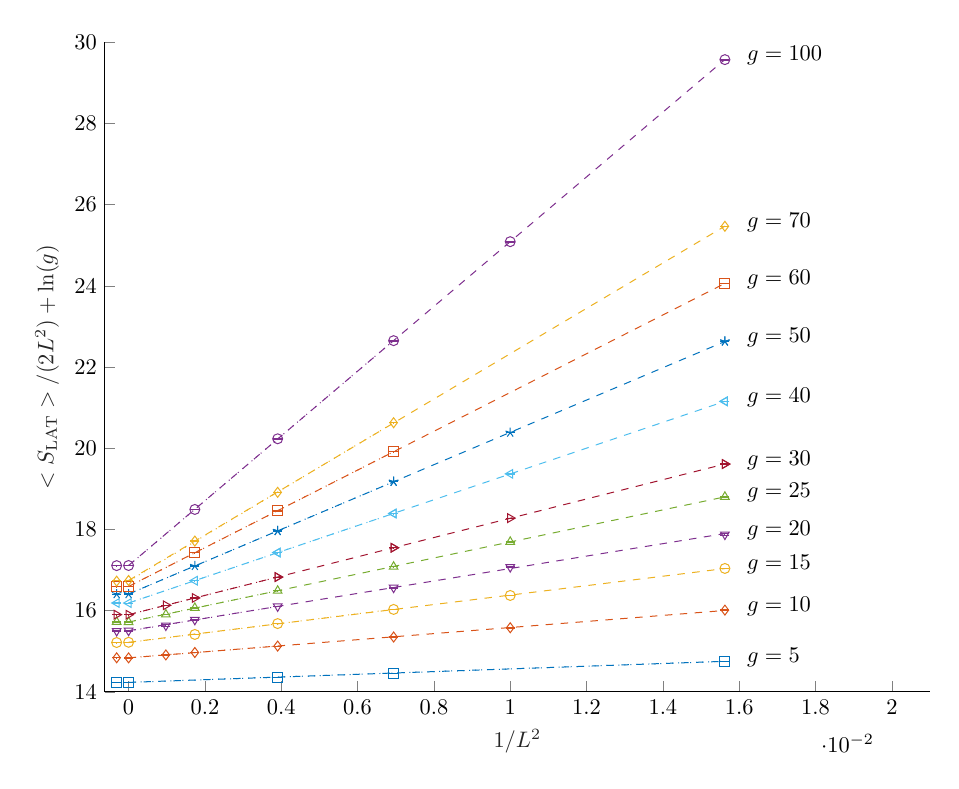
\begin{tikzpicture}[thick,scale=0.9, every node/.style={scale=0.9}]

\begin{axis}[%
width=4.585in,
height=3.608in,
at={(0.769in,0.487in)},
scale only axis,
xmin=-0.000625,
xmax=0.021,
xlabel style={font=\color{white!15!black}},
xlabel={$1/L^2$},
ymin=14,
ymax=30,
ylabel style={font=\color{white!15!black}},
ylabel={$<S_{\rm LAT}> / (2L^2) + \ln(g)$},
axis background/.style={fill=white},
axis x line*=bottom,
axis y line*=left
]
\addplot [color=mycolor1, dotted, forget plot]
  table[row sep=crcr]{%
0	14.2319079966092\\
0.00015625	14.2371004315295\\
0.0003125	14.2422928664499\\
0.00046875	14.2474853013703\\
0.000625	14.2526777362907\\
0.00078125	14.257870171211\\
0.0009375	14.2630626061314\\
0.00109375	14.2682550410518\\
0.00125	14.2734474759722\\
0.00140625	14.2786399108925\\
0.0015625	14.2838323458129\\
0.00171875	14.2890247807333\\
0.001875	14.2942172156537\\
0.00203125	14.299409650574\\
0.0021875	14.3046020854944\\
0.00234375	14.3097945204148\\
0.0025	14.3149869553351\\
0.00265625	14.3201793902555\\
0.0028125	14.3253718251759\\
0.00296875	14.3305642600963\\
0.003125	14.3357566950166\\
0.00328125	14.340949129937\\
0.0034375	14.3461415648574\\
0.00359375	14.3513339997778\\
0.00375	14.3565264346981\\
0.00390625	14.3617188696185\\
0.0040625	14.3669113045389\\
0.00421875	14.3721037394593\\
0.004375	14.3772961743796\\
0.00453125	14.3824886093\\
0.0046875	14.3876810442204\\
0.00484375	14.3928734791407\\
0.005	14.3980659140611\\
0.00515625	14.4032583489815\\
0.0053125	14.4084507839019\\
0.00546875	14.4136432188222\\
0.005625	14.4188356537426\\
0.00578125	14.424028088663\\
0.0059375	14.4292205235834\\
0.00609375	14.4344129585037\\
0.00625	14.4396053934241\\
0.00640625	14.4447978283445\\
0.0065625	14.4499902632648\\
0.00671875	14.4551826981852\\
0.006875	14.4603751331056\\
0.00703125	14.465567568026\\
0.0071875	14.4707600029463\\
0.00734375	14.4759524378667\\
0.0075	14.4811448727871\\
0.00765625	14.4863373077075\\
0.0078125	14.4915297426278\\
0.00796875	14.4967221775482\\
0.008125	14.5019146124686\\
0.00828125	14.507107047389\\
0.0084375	14.5122994823093\\
0.00859375	14.5174919172297\\
0.00875	14.5226843521501\\
0.00890625	14.5278767870704\\
0.0090625	14.5330692219908\\
0.00921875	14.5382616569112\\
0.009375	14.5434540918316\\
0.00953125	14.5486465267519\\
0.0096875	14.5538389616723\\
0.00984375	14.5590313965927\\
0.01	14.5642238315131\\
0.01015625	14.5694162664334\\
0.0103125	14.5746087013538\\
0.01046875	14.5798011362742\\
0.010625	14.5849935711945\\
0.01078125	14.5901860061149\\
0.0109375	14.5953784410353\\
0.01109375	14.6005708759557\\
0.01125	14.605763310876\\
0.01140625	14.6109557457964\\
0.0115625	14.6161481807168\\
0.01171875	14.6213406156372\\
0.011875	14.6265330505575\\
0.01203125	14.6317254854779\\
0.0121875	14.6369179203983\\
0.01234375	14.6421103553186\\
0.0125	14.647302790239\\
0.01265625	14.6524952251594\\
0.0128125	14.6576876600798\\
0.01296875	14.6628800950001\\
0.013125	14.6680725299205\\
0.01328125	14.6732649648409\\
0.0134375	14.6784573997613\\
0.01359375	14.6836498346816\\
0.01375	14.688842269602\\
0.01390625	14.6940347045224\\
0.0140625	14.6992271394428\\
0.01421875	14.7044195743631\\
0.014375	14.7096120092835\\
0.01453125	14.7148044442039\\
0.0146875	14.7199968791242\\
0.01484375	14.7251893140446\\
0.015	14.730381748965\\
0.01515625	14.7355741838854\\
0.0153125	14.7407666188057\\
0.01546875	14.7459590537261\\
0.015625	14.7511514886465\\
};
\addplot [color=mycolor1, dashed, forget plot]
  table[row sep=crcr]{%
0	14.2319079966092\\
0.00015625	14.2371004315295\\
0.0003125	14.2422928664499\\
0.00046875	14.2474853013703\\
0.000625	14.2526777362907\\
0.00078125	14.257870171211\\
0.0009375	14.2630626061314\\
0.00109375	14.2682550410518\\
0.00125	14.2734474759722\\
0.00140625	14.2786399108925\\
0.0015625	14.2838323458129\\
0.00171875	14.2890247807333\\
0.001875	14.2942172156537\\
0.00203125	14.299409650574\\
0.0021875	14.3046020854944\\
0.00234375	14.3097945204148\\
0.0025	14.3149869553351\\
0.00265625	14.3201793902555\\
0.0028125	14.3253718251759\\
0.00296875	14.3305642600963\\
0.003125	14.3357566950166\\
0.00328125	14.340949129937\\
0.0034375	14.3461415648574\\
0.00359375	14.3513339997778\\
0.00375	14.3565264346981\\
0.00390625	14.3617188696185\\
0.0040625	14.3669113045389\\
0.00421875	14.3721037394593\\
0.004375	14.3772961743796\\
0.00453125	14.3824886093\\
0.0046875	14.3876810442204\\
0.00484375	14.3928734791407\\
0.005	14.3980659140611\\
0.00515625	14.4032583489815\\
0.0053125	14.4084507839019\\
0.00546875	14.4136432188222\\
0.005625	14.4188356537426\\
0.00578125	14.424028088663\\
0.0059375	14.4292205235834\\
0.00609375	14.4344129585037\\
0.00625	14.4396053934241\\
0.00640625	14.4447978283445\\
0.0065625	14.4499902632648\\
0.00671875	14.4551826981852\\
0.006875	14.4603751331056\\
0.00703125	14.465567568026\\
0.0071875	14.4707600029463\\
0.00734375	14.4759524378667\\
0.0075	14.4811448727871\\
0.00765625	14.4863373077075\\
0.0078125	14.4915297426278\\
0.00796875	14.4967221775482\\
0.008125	14.5019146124686\\
0.00828125	14.507107047389\\
0.0084375	14.5122994823093\\
0.00859375	14.5174919172297\\
0.00875	14.5226843521501\\
0.00890625	14.5278767870704\\
0.0090625	14.5330692219908\\
0.00921875	14.5382616569112\\
0.009375	14.5434540918316\\
0.00953125	14.5486465267519\\
0.0096875	14.5538389616723\\
0.00984375	14.5590313965927\\
0.01	14.5642238315131\\
0.01015625	14.5694162664334\\
0.0103125	14.5746087013538\\
0.01046875	14.5798011362742\\
0.010625	14.5849935711945\\
0.01078125	14.5901860061149\\
0.0109375	14.5953784410353\\
0.01109375	14.6005708759557\\
0.01125	14.605763310876\\
0.01140625	14.6109557457964\\
0.0115625	14.6161481807168\\
0.01171875	14.6213406156372\\
0.011875	14.6265330505575\\
0.01203125	14.6317254854779\\
0.0121875	14.6369179203983\\
0.01234375	14.6421103553186\\
0.0125	14.647302790239\\
0.01265625	14.6524952251594\\
0.0128125	14.6576876600798\\
0.01296875	14.6628800950001\\
0.013125	14.6680725299205\\
0.01328125	14.6732649648409\\
0.0134375	14.6784573997613\\
0.01359375	14.6836498346816\\
0.01375	14.688842269602\\
0.01390625	14.6940347045224\\
0.0140625	14.6992271394428\\
0.01421875	14.7044195743631\\
0.014375	14.7096120092835\\
0.01453125	14.7148044442039\\
0.0146875	14.7199968791242\\
0.01484375	14.7251893140446\\
0.015	14.730381748965\\
0.01515625	14.7355741838854\\
0.0153125	14.7407666188057\\
0.01546875	14.7459590537261\\
0.015625	14.7511514886465\\
};
\addplot [color=mycolor1, draw=none, mark=square, mark options={solid, mycolor1}, forget plot]
 plot [error bars/.cd, y dir = both, y explicit]
 table[row sep=crcr, y error plus index=2, y error minus index=3]{%
0	14.2319079966092	0.0035673092009017	0.0035673092009017\\
-0.0003125	14.2319079966092	0.0035673092009017	0.0035673092009017\\
0.015625	14.7522190119062	0.00506080096931434	0.00506080096931434\\
0.00694444444444444	14.4610186726407	0.00321737510581956	0.00321737510581956\\
0.00390625	14.3624432909252	0.0024663812740694	0.0024663812740694\\
};
\node[right, align=left]
at (axis cs:0.016,14.852) {$g =   5$};
\addplot [color=mycolor2, dotted, forget plot]
  table[row sep=crcr]{%
0	14.8378735517807\\
0.00015625	14.8494352503866\\
0.0003125	14.8609969489925\\
0.00046875	14.8725586475985\\
0.000625	14.8841203462044\\
0.00078125	14.8956820448103\\
0.0009375	14.9072437434163\\
0.00109375	14.9188054420222\\
0.00125	14.9303671406282\\
0.00140625	14.9419288392341\\
0.0015625	14.95349053784\\
0.00171875	14.965052236446\\
0.001875	14.9766139350519\\
0.00203125	14.9881756336578\\
0.0021875	14.9997373322638\\
0.00234375	15.0112990308697\\
0.0025	15.0228607294756\\
0.00265625	15.0344224280816\\
0.0028125	15.0459841266875\\
0.00296875	15.0575458252934\\
0.003125	15.0691075238994\\
0.00328125	15.0806692225053\\
0.0034375	15.0922309211113\\
0.00359375	15.1037926197172\\
0.00375	15.1153543183231\\
0.00390625	15.1269160169291\\
};
\addplot [color=mycolor2, dashed, forget plot]
  table[row sep=crcr]{%
0	14.8358915276158\\
0.00015625	14.8475701150126\\
0.0003125	14.8592487024095\\
0.00046875	14.8709272898063\\
0.000625	14.8826058772032\\
0.00078125	14.8942844646001\\
0.0009375	14.9059630519969\\
0.00109375	14.9176416393938\\
0.00125	14.9293202267907\\
0.00140625	14.9409988141875\\
0.0015625	14.9526774015844\\
0.00171875	14.9643559889812\\
0.001875	14.9760345763781\\
0.00203125	14.987713163775\\
0.0021875	14.9993917511718\\
0.00234375	15.0110703385687\\
0.0025	15.0227489259655\\
0.00265625	15.0344275133624\\
0.0028125	15.0461061007593\\
0.00296875	15.0577846881561\\
0.003125	15.069463275553\\
0.00328125	15.0811418629499\\
0.0034375	15.0928204503467\\
0.00359375	15.1044990377436\\
0.00375	15.1161776251404\\
0.00390625	15.1278562125373\\
0.0040625	15.1395347999342\\
0.00421875	15.151213387331\\
0.004375	15.1628919747279\\
0.00453125	15.1745705621247\\
0.0046875	15.1862491495216\\
0.00484375	15.1979277369185\\
0.005	15.2096063243153\\
0.00515625	15.2212849117122\\
0.0053125	15.2329634991091\\
0.00546875	15.2446420865059\\
0.005625	15.2563206739028\\
0.00578125	15.2679992612996\\
0.0059375	15.2796778486965\\
0.00609375	15.2913564360934\\
0.00625	15.3030350234902\\
0.00640625	15.3147136108871\\
0.0065625	15.3263921982839\\
0.00671875	15.3380707856808\\
0.006875	15.3497493730777\\
0.00703125	15.3614279604745\\
0.0071875	15.3731065478714\\
0.00734375	15.3847851352683\\
0.0075	15.3964637226651\\
0.00765625	15.408142310062\\
0.0078125	15.4198208974588\\
0.00796875	15.4314994848557\\
0.008125	15.4431780722526\\
0.00828125	15.4548566596494\\
0.0084375	15.4665352470463\\
0.00859375	15.4782138344431\\
0.00875	15.48989242184\\
0.00890625	15.5015710092369\\
0.0090625	15.5132495966337\\
0.00921875	15.5249281840306\\
0.009375	15.5366067714275\\
0.00953125	15.5482853588243\\
0.0096875	15.5599639462212\\
0.00984375	15.571642533618\\
0.01	15.5833211210149\\
0.01015625	15.5949997084118\\
0.0103125	15.6066782958086\\
0.01046875	15.6183568832055\\
0.010625	15.6300354706024\\
0.01078125	15.6417140579992\\
0.0109375	15.6533926453961\\
0.01109375	15.6650712327929\\
0.01125	15.6767498201898\\
0.01140625	15.6884284075867\\
0.0115625	15.7001069949835\\
0.01171875	15.7117855823804\\
0.011875	15.7234641697772\\
0.01203125	15.7351427571741\\
0.0121875	15.746821344571\\
0.01234375	15.7584999319678\\
0.0125	15.7701785193647\\
0.01265625	15.7818571067615\\
0.0128125	15.7935356941584\\
0.01296875	15.8052142815553\\
0.013125	15.8168928689521\\
0.01328125	15.828571456349\\
0.0134375	15.8402500437459\\
0.01359375	15.8519286311427\\
0.01375	15.8636072185396\\
0.01390625	15.8752858059364\\
0.0140625	15.8869643933333\\
0.01421875	15.8986429807302\\
0.014375	15.910321568127\\
0.01453125	15.9220001555239\\
0.0146875	15.9336787429208\\
0.01484375	15.9453573303176\\
0.015	15.9570359177145\\
0.01515625	15.9687145051113\\
0.0153125	15.9803930925082\\
0.01546875	15.9920716799051\\
0.015625	16.0037502673019\\
};
\addplot [color=mycolor2, draw=none, mark=diamond, mark options={solid, mycolor2}, forget plot]
 plot [error bars/.cd, y dir = both, y explicit]
 table[row sep=crcr, y error plus index=2, y error minus index=3]{%
0	14.8358915276158	0.00191119909436733	0.00191119909436733\\
-0.0003125	14.8378735517807	0.00310308956262772	0.00310308956262772\\
0.015625	16.0126699376744	0.00649678356734707	0.00649678356734707\\
0.01	15.5783738649342	0.00576032943715814	0.00576032943715814\\
0.00694444444444444	15.3490362078809	0.00480069134079562	0.00480069134079562\\
0.00390625	15.1261092353046	0.00293682794744704	0.00293682794744704\\
0.00173611111111111	14.968249843279	0.00230261928550103	0.00230261928550103\\
0.0009765625	14.9082127754043	0.00268128261035795	0.00268128261035795\\
};
\node[right, align=left]
at (axis cs:0.016,16.113) {$g =  10$};
\addplot [color=mycolor3, dotted, forget plot]
  table[row sep=crcr]{%
0	15.2143179687161\\
0.00015625	15.2327370518638\\
0.0003125	15.2511561350115\\
0.00046875	15.2695752181591\\
0.000625	15.2879943013068\\
0.00078125	15.3064133844545\\
0.0009375	15.3248324676021\\
0.00109375	15.3432515507498\\
0.00125	15.3616706338974\\
0.00140625	15.3800897170451\\
0.0015625	15.3985088001928\\
0.00171875	15.4169278833404\\
0.001875	15.4353469664881\\
0.00203125	15.4537660496358\\
0.0021875	15.4721851327834\\
0.00234375	15.4906042159311\\
0.0025	15.5090232990787\\
0.00265625	15.5274423822264\\
0.0028125	15.5458614653741\\
0.00296875	15.5642805485217\\
0.003125	15.5826996316694\\
0.00328125	15.601118714817\\
0.0034375	15.6195377979647\\
0.00359375	15.6379568811124\\
0.00375	15.65637596426\\
0.00390625	15.6747950474077\\
0.0040625	15.6932141305554\\
0.00421875	15.711633213703\\
0.004375	15.7300522968507\\
0.00453125	15.7484713799983\\
0.0046875	15.766890463146\\
0.00484375	15.7853095462937\\
0.005	15.8037286294413\\
0.00515625	15.822147712589\\
0.0053125	15.8405667957367\\
0.00546875	15.8589858788843\\
0.005625	15.877404962032\\
0.00578125	15.8958240451796\\
0.0059375	15.9142431283273\\
0.00609375	15.932662211475\\
0.00625	15.9510812946226\\
0.00640625	15.9695003777703\\
0.0065625	15.987919460918\\
0.00671875	16.0063385440656\\
0.006875	16.0247576272133\\
};
\addplot [color=mycolor3, dashed, forget plot]
  table[row sep=crcr]{%
0	15.2197915592611\\
0.00015625	15.2379578250624\\
0.0003125	15.2561240908637\\
0.00046875	15.274290356665\\
0.000625	15.2924566224663\\
0.00078125	15.3106228882676\\
0.0009375	15.3287891540689\\
0.00109375	15.3469554198702\\
0.00125	15.3651216856715\\
0.00140625	15.3832879514727\\
0.0015625	15.401454217274\\
0.00171875	15.4196204830753\\
0.001875	15.4377867488766\\
0.00203125	15.4559530146779\\
0.0021875	15.4741192804792\\
0.00234375	15.4922855462805\\
0.0025	15.5104518120818\\
0.00265625	15.5286180778831\\
0.0028125	15.5467843436844\\
0.00296875	15.5649506094857\\
0.003125	15.5831168752869\\
0.00328125	15.6012831410882\\
0.0034375	15.6194494068895\\
0.00359375	15.6376156726908\\
0.00375	15.6557819384921\\
0.00390625	15.6739482042934\\
0.0040625	15.6921144700947\\
0.00421875	15.710280735896\\
0.004375	15.7284470016973\\
0.00453125	15.7466132674986\\
0.0046875	15.7647795332998\\
0.00484375	15.7829457991011\\
0.005	15.8011120649024\\
0.00515625	15.8192783307037\\
0.0053125	15.837444596505\\
0.00546875	15.8556108623063\\
0.005625	15.8737771281076\\
0.00578125	15.8919433939089\\
0.0059375	15.9101096597102\\
0.00609375	15.9282759255115\\
0.00625	15.9464421913128\\
0.00640625	15.964608457114\\
0.0065625	15.9827747229153\\
0.00671875	16.0009409887166\\
0.006875	16.0191072545179\\
0.00703125	16.0372735203192\\
0.0071875	16.0554397861205\\
0.00734375	16.0736060519218\\
0.0075	16.0917723177231\\
0.00765625	16.1099385835244\\
0.0078125	16.1281048493257\\
0.00796875	16.146271115127\\
0.008125	16.1644373809282\\
0.00828125	16.1826036467295\\
0.0084375	16.2007699125308\\
0.00859375	16.2189361783321\\
0.00875	16.2371024441334\\
0.00890625	16.2552687099347\\
0.0090625	16.273434975736\\
0.00921875	16.2916012415373\\
0.009375	16.3097675073386\\
0.00953125	16.3279337731399\\
0.0096875	16.3461000389411\\
0.00984375	16.3642663047424\\
0.01	16.3824325705437\\
0.01015625	16.400598836345\\
0.0103125	16.4187651021463\\
0.01046875	16.4369313679476\\
0.010625	16.4550976337489\\
0.01078125	16.4732638995502\\
0.0109375	16.4914301653515\\
0.01109375	16.5095964311528\\
0.01125	16.527762696954\\
0.01140625	16.5459289627553\\
0.0115625	16.5640952285566\\
0.01171875	16.5822614943579\\
0.011875	16.6004277601592\\
0.01203125	16.6185940259605\\
0.0121875	16.6367602917618\\
0.01234375	16.6549265575631\\
0.0125	16.6730928233644\\
0.01265625	16.6912590891657\\
0.0128125	16.709425354967\\
0.01296875	16.7275916207682\\
0.013125	16.7457578865695\\
0.01328125	16.7639241523708\\
0.0134375	16.7820904181721\\
0.01359375	16.8002566839734\\
0.01375	16.8184229497747\\
0.01390625	16.836589215576\\
0.0140625	16.8547554813773\\
0.01421875	16.8729217471786\\
0.014375	16.8910880129799\\
0.01453125	16.9092542787812\\
0.0146875	16.9274205445824\\
0.01484375	16.9455868103837\\
0.015	16.963753076185\\
0.01515625	16.9819193419863\\
0.0153125	17.0000856077876\\
0.01546875	17.0182518735889\\
0.015625	17.0364181393902\\
};
\addplot [color=mycolor3, draw=none, mark=o, mark options={solid, mycolor3}, forget plot]
 plot [error bars/.cd, y dir = both, y explicit]
 table[row sep=crcr, y error plus index=2, y error minus index=3]{%
0	15.2197915592611	0.00546179104759107	0.00546179104759107\\
-0.0003125	15.2143179687161	0.00816245596563924	0.00816245596563924\\
0.015625	17.0389028992136	0.00956196090019351	0.00956196090019351\\
0.01	16.373714034043	0.00768250137502182	0.00768250137502182\\
0.00694444444444444	16.0293672322996	0.00621551833694698	0.00621551833694698\\
0.00390625	15.68094696326	0.00526184988918465	0.00526184988918465\\
0.00173611111111111	15.4131417428843	0.00670825988521705	0.00670825988521705\\
};
\node[right, align=left]
at (axis cs:0.016,17.139) {$g =  15$};
\addplot [color=mycolor4, dotted, forget plot]
  table[row sep=crcr]{%
0	15.4979244830486\\
0.00015625	15.5221620156008\\
0.0003125	15.5463995481529\\
0.00046875	15.5706370807051\\
0.000625	15.5948746132572\\
0.00078125	15.6191121458094\\
0.0009375	15.6433496783615\\
0.00109375	15.6675872109137\\
0.00125	15.6918247434658\\
0.00140625	15.716062276018\\
0.0015625	15.7402998085701\\
0.00171875	15.7645373411223\\
0.001875	15.7887748736744\\
0.00203125	15.8130124062266\\
0.0021875	15.8372499387787\\
0.00234375	15.8614874713309\\
0.0025	15.885725003883\\
0.00265625	15.9099625364352\\
0.0028125	15.9342000689873\\
0.00296875	15.9584376015395\\
0.003125	15.9826751340916\\
0.00328125	16.0069126666438\\
0.0034375	16.031150199196\\
0.00359375	16.0553877317481\\
0.00375	16.0796252643003\\
0.00390625	16.1038627968524\\
};
\addplot [color=mycolor4, dashed, forget plot]
  table[row sep=crcr]{%
0	15.5050076924797\\
0.00015625	15.5289457349157\\
0.0003125	15.5528837773518\\
0.00046875	15.5768218197878\\
0.000625	15.6007598622238\\
0.00078125	15.6246979046599\\
0.0009375	15.6486359470959\\
0.00109375	15.6725739895319\\
0.00125	15.696512031968\\
0.00140625	15.720450074404\\
0.0015625	15.74438811684\\
0.00171875	15.7683261592761\\
0.001875	15.7922642017121\\
0.00203125	15.8162022441481\\
0.0021875	15.8401402865842\\
0.00234375	15.8640783290202\\
0.0025	15.8880163714562\\
0.00265625	15.9119544138923\\
0.0028125	15.9358924563283\\
0.00296875	15.9598304987643\\
0.003125	15.9837685412004\\
0.00328125	16.0077065836364\\
0.0034375	16.0316446260724\\
0.00359375	16.0555826685085\\
0.00375	16.0795207109445\\
0.00390625	16.1034587533805\\
0.0040625	16.1273967958166\\
0.00421875	16.1513348382526\\
0.004375	16.1752728806886\\
0.00453125	16.1992109231247\\
0.0046875	16.2231489655607\\
0.00484375	16.2470870079967\\
0.005	16.2710250504328\\
0.00515625	16.2949630928688\\
0.0053125	16.3189011353048\\
0.00546875	16.3428391777409\\
0.005625	16.3667772201769\\
0.00578125	16.3907152626129\\
0.0059375	16.414653305049\\
0.00609375	16.438591347485\\
0.00625	16.462529389921\\
0.00640625	16.4864674323571\\
0.0065625	16.5104054747931\\
0.00671875	16.5343435172291\\
0.006875	16.5582815596652\\
0.00703125	16.5822196021012\\
0.0071875	16.6061576445372\\
0.00734375	16.6300956869733\\
0.0075	16.6540337294093\\
0.00765625	16.6779717718453\\
0.0078125	16.7019098142814\\
0.00796875	16.7258478567174\\
0.008125	16.7497858991534\\
0.00828125	16.7737239415895\\
0.0084375	16.7976619840255\\
0.00859375	16.8216000264615\\
0.00875	16.8455380688976\\
0.00890625	16.8694761113336\\
0.0090625	16.8934141537696\\
0.00921875	16.9173521962057\\
0.009375	16.9412902386417\\
0.00953125	16.9652282810777\\
0.0096875	16.9891663235138\\
0.00984375	17.0131043659498\\
0.01	17.0370424083858\\
0.01015625	17.0609804508219\\
0.0103125	17.0849184932579\\
0.01046875	17.1088565356939\\
0.010625	17.13279457813\\
0.01078125	17.156732620566\\
0.0109375	17.180670663002\\
0.01109375	17.2046087054381\\
0.01125	17.2285467478741\\
0.01140625	17.2524847903101\\
0.0115625	17.2764228327462\\
0.01171875	17.3003608751822\\
0.011875	17.3242989176182\\
0.01203125	17.3482369600543\\
0.0121875	17.3721750024903\\
0.01234375	17.3961130449263\\
0.0125	17.4200510873624\\
0.01265625	17.4439891297984\\
0.0128125	17.4679271722344\\
0.01296875	17.4918652146705\\
0.013125	17.5158032571065\\
0.01328125	17.5397412995425\\
0.0134375	17.5636793419786\\
0.01359375	17.5876173844146\\
0.01375	17.6115554268506\\
0.01390625	17.6354934692867\\
0.0140625	17.6594315117227\\
0.01421875	17.6833695541587\\
0.014375	17.7073075965947\\
0.01453125	17.7312456390308\\
0.0146875	17.7551836814668\\
0.01484375	17.7791217239029\\
0.015	17.8030597663389\\
0.01515625	17.8269978087749\\
0.0153125	17.8509358512109\\
0.01546875	17.874873893647\\
0.015625	17.898811936083\\
};
\addplot [color=mycolor4, draw=none, mark=triangle, mark options={solid, rotate=180, mycolor4}, forget plot]
 plot [error bars/.cd, y dir = both, y explicit]
 table[row sep=crcr, y error plus index=2, y error minus index=3]{%
0	15.5050076924797	0.00943604846448236	0.00943604846448236\\
-0.0003125	15.4979244830486	0.0186305960254734	0.0186305960254734\\
0.015625	17.8734890391786	0.0191712158191764	0.0191712158191764\\
0.01	17.0719267420178	0.0161283634880507	0.0161283634880507\\
0.00694444444444444	16.5650169747978	0.011031391627096	0.011031391627096\\
0.00390625	16.1027126978765	0.0101268417209217	0.0101268417209217\\
0.00173611111111111	15.7731239327551	0.0116724330509517	0.0116724330509517\\
0.0009765625	15.6318391473476	0.0234166764718092	0.0234166764718092\\
};
\node[right, align=left]
at (axis cs:0.016,17.973) {$g =  20$};
\addplot [color=mycolor5, dotted, forget plot]
  table[row sep=crcr]{%
0	15.7224225066749\\
0.00015625	15.753121222769\\
0.0003125	15.7838199388631\\
0.00046875	15.8145186549572\\
0.000625	15.8452173710513\\
0.00078125	15.8759160871454\\
0.0009375	15.9066148032395\\
0.00109375	15.9373135193336\\
0.00125	15.9680122354277\\
0.00140625	15.9987109515218\\
0.0015625	16.0294096676159\\
0.00171875	16.06010838371\\
0.001875	16.0908070998041\\
0.00203125	16.1215058158982\\
0.0021875	16.1522045319923\\
0.00234375	16.1829032480864\\
0.0025	16.2136019641805\\
0.00265625	16.2443006802746\\
0.0028125	16.2749993963687\\
0.00296875	16.3056981124627\\
0.003125	16.3363968285568\\
0.00328125	16.3670955446509\\
0.0034375	16.397794260745\\
0.00359375	16.4284929768391\\
0.00375	16.4591916929332\\
0.00390625	16.4898904090273\\
};
\addplot [color=mycolor5, dashed, forget plot]
  table[row sep=crcr]{%
0	15.7185084306154\\
0.00015625	15.7493426199827\\
0.0003125	15.78017680935\\
0.00046875	15.8110109987173\\
0.000625	15.8418451880846\\
0.00078125	15.8726793774519\\
0.0009375	15.9035135668191\\
0.00109375	15.9343477561864\\
0.00125	15.9651819455537\\
0.00140625	15.996016134921\\
0.0015625	16.0268503242883\\
0.00171875	16.0576845136556\\
0.001875	16.0885187030229\\
0.00203125	16.1193528923901\\
0.0021875	16.1501870817574\\
0.00234375	16.1810212711247\\
0.0025	16.211855460492\\
0.00265625	16.2426896498593\\
0.0028125	16.2735238392266\\
0.00296875	16.3043580285939\\
0.003125	16.3351922179612\\
0.00328125	16.3660264073284\\
0.0034375	16.3968605966957\\
0.00359375	16.427694786063\\
0.00375	16.4585289754303\\
0.00390625	16.4893631647976\\
0.0040625	16.5201973541649\\
0.00421875	16.5510315435322\\
0.004375	16.5818657328994\\
0.00453125	16.6126999222667\\
0.0046875	16.643534111634\\
0.00484375	16.6743683010013\\
0.005	16.7052024903686\\
0.00515625	16.7360366797359\\
0.0053125	16.7668708691032\\
0.00546875	16.7977050584704\\
0.005625	16.8285392478377\\
0.00578125	16.859373437205\\
0.0059375	16.8902076265723\\
0.00609375	16.9210418159396\\
0.00625	16.9518760053069\\
0.00640625	16.9827101946742\\
0.0065625	17.0135443840414\\
0.00671875	17.0443785734087\\
0.006875	17.075212762776\\
0.00703125	17.1060469521433\\
0.0071875	17.1368811415106\\
0.00734375	17.1677153308779\\
0.0075	17.1985495202452\\
0.00765625	17.2293837096125\\
0.0078125	17.2602178989797\\
0.00796875	17.291052088347\\
0.008125	17.3218862777143\\
0.00828125	17.3527204670816\\
0.0084375	17.3835546564489\\
0.00859375	17.4143888458162\\
0.00875	17.4452230351835\\
0.00890625	17.4760572245507\\
0.0090625	17.506891413918\\
0.00921875	17.5377256032853\\
0.009375	17.5685597926526\\
0.00953125	17.5993939820199\\
0.0096875	17.6302281713872\\
0.00984375	17.6610623607545\\
0.01	17.6918965501217\\
0.01015625	17.722730739489\\
0.0103125	17.7535649288563\\
0.01046875	17.7843991182236\\
0.010625	17.8152333075909\\
0.01078125	17.8460674969582\\
0.0109375	17.8769016863255\\
0.01109375	17.9077358756928\\
0.01125	17.93857006506\\
0.01140625	17.9694042544273\\
0.0115625	18.0002384437946\\
0.01171875	18.0310726331619\\
0.011875	18.0619068225292\\
0.01203125	18.0927410118965\\
0.0121875	18.1235752012638\\
0.01234375	18.154409390631\\
0.0125	18.1852435799983\\
0.01265625	18.2160777693656\\
0.0128125	18.2469119587329\\
0.01296875	18.2777461481002\\
0.013125	18.3085803374675\\
0.01328125	18.3394145268348\\
0.0134375	18.370248716202\\
0.01359375	18.4010829055693\\
0.01375	18.4319170949366\\
0.01390625	18.4627512843039\\
0.0140625	18.4935854736712\\
0.01421875	18.5244196630385\\
0.014375	18.5552538524058\\
0.01453125	18.586088041773\\
0.0146875	18.6169222311403\\
0.01484375	18.6477564205076\\
0.015	18.6785906098749\\
0.01515625	18.7094247992422\\
0.0153125	18.7402589886095\\
0.01546875	18.7710931779768\\
0.015625	18.8019273673441\\
};
\addplot [color=mycolor5, draw=none, mark=triangle, mark options={solid, mycolor5}, forget plot]
 plot [error bars/.cd, y dir = both, y explicit]
 table[row sep=crcr, y error plus index=2, y error minus index=3]{%
0	15.7185084306154	0.00262893477657402	0.00262893477657402\\
-0.0003125	15.7224225066749	0.00558645908897847	0.00558645908897847\\
0.015625	18.804847155296	0.00499060920711709	0.00499060920711709\\
0.01	17.6951413892682	0.00406705036469493	0.00406705036469493\\
0.00694444444444444	17.0817923533826	0.0033094804721687	0.0033094804721687\\
0.00390625	16.489553271165	0.00255846333284774	0.00255846333284774\\
0.00173611111111111	16.0658108311243	0.00339625669562994	0.00339625669562994\\
0.0009765625	15.904825677063	0.00801940876909065	0.00801940876909065\\
};
\node[right, align=left]
at (axis cs:0.016,18.905) {$g =  25$};
\addplot [color=mycolor6, dotted, forget plot]
  table[row sep=crcr]{%
0	15.9005865177977\\
0.00015625	15.9376394543882\\
0.0003125	15.9746923909787\\
0.00046875	16.0117453275693\\
0.000625	16.0487982641598\\
0.00078125	16.0858512007504\\
0.0009375	16.1229041373409\\
0.00109375	16.1599570739314\\
0.00125	16.197010010522\\
0.00140625	16.2340629471125\\
0.0015625	16.2711158837031\\
0.00171875	16.3081688202936\\
0.001875	16.3452217568841\\
0.00203125	16.3822746934747\\
0.0021875	16.4193276300652\\
0.00234375	16.4563805666558\\
0.0025	16.4934335032463\\
0.00265625	16.5304864398369\\
0.0028125	16.5675393764274\\
0.00296875	16.6045923130179\\
0.003125	16.6416452496085\\
0.00328125	16.678698186199\\
0.0034375	16.7157511227896\\
0.00359375	16.7528040593801\\
0.00375	16.7898569959706\\
0.00390625	16.8269099325612\\
};
\addplot [color=mycolor6, dashed, forget plot]
  table[row sep=crcr]{%
0	15.8996524495376\\
0.00015625	15.9367740629237\\
0.0003125	15.9738956763098\\
0.00046875	16.0110172896959\\
0.000625	16.048138903082\\
0.00078125	16.085260516468\\
0.0009375	16.1223821298541\\
0.00109375	16.1595037432402\\
0.00125	16.1966253566263\\
0.00140625	16.2337469700124\\
0.0015625	16.2708685833984\\
0.00171875	16.3079901967845\\
0.001875	16.3451118101706\\
0.00203125	16.3822334235567\\
0.0021875	16.4193550369428\\
0.00234375	16.4564766503288\\
0.0025	16.4935982637149\\
0.00265625	16.530719877101\\
0.0028125	16.5678414904871\\
0.00296875	16.6049631038732\\
0.003125	16.6420847172593\\
0.00328125	16.6792063306453\\
0.0034375	16.7163279440314\\
0.00359375	16.7534495574175\\
0.00375	16.7905711708036\\
0.00390625	16.8276927841897\\
0.0040625	16.8648143975757\\
0.00421875	16.9019360109618\\
0.004375	16.9390576243479\\
0.00453125	16.976179237734\\
0.0046875	17.0133008511201\\
0.00484375	17.0504224645061\\
0.005	17.0875440778922\\
0.00515625	17.1246656912783\\
0.0053125	17.1617873046644\\
0.00546875	17.1989089180505\\
0.005625	17.2360305314365\\
0.00578125	17.2731521448226\\
0.0059375	17.3102737582087\\
0.00609375	17.3473953715948\\
0.00625	17.3845169849809\\
0.00640625	17.421638598367\\
0.0065625	17.458760211753\\
0.00671875	17.4958818251391\\
0.006875	17.5330034385252\\
0.00703125	17.5701250519113\\
0.0071875	17.6072466652974\\
0.00734375	17.6443682786834\\
0.0075	17.6814898920695\\
0.00765625	17.7186115054556\\
0.0078125	17.7557331188417\\
0.00796875	17.7928547322278\\
0.008125	17.8299763456138\\
0.00828125	17.8670979589999\\
0.0084375	17.904219572386\\
0.00859375	17.9413411857721\\
0.00875	17.9784627991582\\
0.00890625	18.0155844125442\\
0.0090625	18.0527060259303\\
0.00921875	18.0898276393164\\
0.009375	18.1269492527025\\
0.00953125	18.1640708660886\\
0.0096875	18.2011924794746\\
0.00984375	18.2383140928607\\
0.01	18.2754357062468\\
0.01015625	18.3125573196329\\
0.0103125	18.349678933019\\
0.01046875	18.3868005464051\\
0.010625	18.4239221597911\\
0.01078125	18.4610437731772\\
0.0109375	18.4981653865633\\
0.01109375	18.5352869999494\\
0.01125	18.5724086133355\\
0.01140625	18.6095302267215\\
0.0115625	18.6466518401076\\
0.01171875	18.6837734534937\\
0.011875	18.7208950668798\\
0.01203125	18.7580166802659\\
0.0121875	18.7951382936519\\
0.01234375	18.832259907038\\
0.0125	18.8693815204241\\
0.01265625	18.9065031338102\\
0.0128125	18.9436247471963\\
0.01296875	18.9807463605823\\
0.013125	19.0178679739684\\
0.01328125	19.0549895873545\\
0.0134375	19.0921112007406\\
0.01359375	19.1292328141267\\
0.01375	19.1663544275127\\
0.01390625	19.2034760408988\\
0.0140625	19.2405976542849\\
0.01421875	19.277719267671\\
0.014375	19.3148408810571\\
0.01453125	19.3519624944432\\
0.0146875	19.3890841078292\\
0.01484375	19.4262057212153\\
0.015	19.4633273346014\\
0.01515625	19.5004489479875\\
0.0153125	19.5375705613736\\
0.01546875	19.5746921747596\\
0.015625	19.6118137881457\\
};
\addplot [color=mycolor6, draw=none, mark=triangle, mark options={solid, rotate=270, mycolor6}, forget plot]
 plot [error bars/.cd, y dir = both, y explicit]
 table[row sep=crcr, y error plus index=2, y error minus index=3]{%
0	15.8996524495376	0.00107274344858564	0.00107274344858564\\
-0.0003125	15.9005865177977	0.00199622968846732	0.00199622968846732\\
0.015625	19.6091391394879	0.00349911613164148	0.00349911613164148\\
0.01	18.2787412738342	0.00260816060732222	0.00260816060732222\\
0.00694444444444444	17.5494632481493	0.00216999038994889	0.00216999038994889\\
0.00390625	16.8269781942745	0.00167103055602843	0.00167103055602843\\
0.00173611111111111	16.3124728788909	0.00110761588993018	0.00110761588993018\\
0.0009765625	16.1313937896946	0.00261705088261531	0.00261705088261531\\
0.015625	19.6128847395535	0.00440248924076026	0.00440248924076026\\
0.00694444444444444	17.5481080338614	0.0028948514373073	0.0028948514373073\\
0.00390625	16.8262910220932	0.00311027013990257	0.00311027013990257\\
};
\node[right, align=left]
at (axis cs:0.016,19.709) {$g =  30$};
\addplot [color=mycolor7, dotted, forget plot]
  table[row sep=crcr]{%
0	16.1878081536208\\
0.00015625	16.2374443329388\\
0.0003125	16.2870805122569\\
0.00046875	16.3367166915749\\
0.000625	16.386352870893\\
0.00078125	16.4359890502111\\
0.0009375	16.4856252295291\\
0.00109375	16.5352614088472\\
0.00125	16.5848975881653\\
0.00140625	16.6345337674833\\
0.0015625	16.6841699468014\\
0.00171875	16.7338061261195\\
0.001875	16.7834423054375\\
0.00203125	16.8330784847556\\
0.0021875	16.8827146640736\\
0.00234375	16.9323508433917\\
0.0025	16.9819870227098\\
0.00265625	17.0316232020278\\
0.0028125	17.0812593813459\\
0.00296875	17.130895560664\\
0.003125	17.180531739982\\
0.00328125	17.2301679193001\\
0.0034375	17.2798040986182\\
0.00359375	17.3294402779362\\
0.00375	17.3790764572543\\
0.00390625	17.4287126365724\\
0.0040625	17.4783488158904\\
0.00421875	17.5279849952085\\
0.004375	17.5776211745265\\
0.00453125	17.6272573538446\\
0.0046875	17.6768935331627\\
0.00484375	17.7265297124807\\
0.005	17.7761658917988\\
0.00515625	17.8258020711169\\
0.0053125	17.8754382504349\\
0.00546875	17.925074429753\\
0.005625	17.9747106090711\\
0.00578125	18.0243467883891\\
0.0059375	18.0739829677072\\
0.00609375	18.1236191470253\\
0.00625	18.1732553263433\\
0.00640625	18.2228915056614\\
0.0065625	18.2725276849794\\
0.00671875	18.3221638642975\\
0.006875	18.3718000436156\\
};
\addplot [color=mycolor7, dashed, forget plot]
  table[row sep=crcr]{%
0	16.1864867474014\\
0.00015625	16.2361795250578\\
0.0003125	16.2858723027141\\
0.00046875	16.3355650803704\\
0.000625	16.3852578580268\\
0.00078125	16.4349506356831\\
0.0009375	16.4846434133394\\
0.00109375	16.5343361909957\\
0.00125	16.5840289686521\\
0.00140625	16.6337217463084\\
0.0015625	16.6834145239647\\
0.00171875	16.7331073016211\\
0.001875	16.7828000792774\\
0.00203125	16.8324928569337\\
0.0021875	16.8821856345901\\
0.00234375	16.9318784122464\\
0.0025	16.9815711899027\\
0.00265625	17.031263967559\\
0.0028125	17.0809567452154\\
0.00296875	17.1306495228717\\
0.003125	17.180342300528\\
0.00328125	17.2300350781844\\
0.0034375	17.2797278558407\\
0.00359375	17.329420633497\\
0.00375	17.3791134111534\\
0.00390625	17.4288061888097\\
0.0040625	17.478498966466\\
0.00421875	17.5281917441223\\
0.004375	17.5778845217787\\
0.00453125	17.627577299435\\
0.0046875	17.6772700770913\\
0.00484375	17.7269628547477\\
0.005	17.776655632404\\
0.00515625	17.8263484100603\\
0.0053125	17.8760411877167\\
0.00546875	17.925733965373\\
0.005625	17.9754267430293\\
0.00578125	18.0251195206857\\
0.0059375	18.074812298342\\
0.00609375	18.1245050759983\\
0.00625	18.1741978536546\\
0.00640625	18.223890631311\\
0.0065625	18.2735834089673\\
0.00671875	18.3232761866236\\
0.006875	18.37296896428\\
0.00703125	18.4226617419363\\
0.0071875	18.4723545195926\\
0.00734375	18.522047297249\\
0.0075	18.5717400749053\\
0.00765625	18.6214328525616\\
0.0078125	18.6711256302179\\
0.00796875	18.7208184078743\\
0.008125	18.7705111855306\\
0.00828125	18.8202039631869\\
0.0084375	18.8698967408433\\
0.00859375	18.9195895184996\\
0.00875	18.9692822961559\\
0.00890625	19.0189750738123\\
0.0090625	19.0686678514686\\
0.00921875	19.1183606291249\\
0.009375	19.1680534067812\\
0.00953125	19.2177461844376\\
0.0096875	19.2674389620939\\
0.00984375	19.3171317397502\\
0.01	19.3668245174066\\
0.01015625	19.4165172950629\\
0.0103125	19.4662100727192\\
0.01046875	19.5159028503756\\
0.010625	19.5655956280319\\
0.01078125	19.6152884056882\\
0.0109375	19.6649811833445\\
0.01109375	19.7146739610009\\
0.01125	19.7643667386572\\
0.01140625	19.8140595163135\\
0.0115625	19.8637522939699\\
0.01171875	19.9134450716262\\
0.011875	19.9631378492825\\
0.01203125	20.0128306269389\\
0.0121875	20.0625234045952\\
0.01234375	20.1122161822515\\
0.0125	20.1619089599079\\
0.01265625	20.2116017375642\\
0.0128125	20.2612945152205\\
0.01296875	20.3109872928768\\
0.013125	20.3606800705332\\
0.01328125	20.4103728481895\\
0.0134375	20.4600656258458\\
0.01359375	20.5097584035022\\
0.01375	20.5594511811585\\
0.01390625	20.6091439588148\\
0.0140625	20.6588367364712\\
0.01421875	20.7085295141275\\
0.014375	20.7582222917838\\
0.01453125	20.8079150694401\\
0.0146875	20.8576078470965\\
0.01484375	20.9073006247528\\
0.015	20.9569934024091\\
0.01515625	21.0066861800655\\
0.0153125	21.0563789577218\\
0.01546875	21.1060717353781\\
0.015625	21.1557645130345\\
};
\addplot [color=mycolor7, draw=none, mark=triangle, mark options={solid, rotate=90, mycolor7}, forget plot]
 plot [error bars/.cd, y dir = both, y explicit]
 table[row sep=crcr, y error plus index=2, y error minus index=3]{%
0	16.1864867474014	0.00123483678129764	0.00123483678129764\\
-0.0003125	16.1878081536208	0.00192282036806188	0.00192282036806188\\
0.015625	21.1538711409765	0.00244730668252586	0.00244730668252586\\
0.01	19.3692491859741	0.00212084349680404	0.00212084349680404\\
0.00694444444444444	18.3932863872867	0.00170093056453765	0.00170093056453765\\
0.00390625	17.4299436427044	0.00123927398558643	0.00123927398558643\\
0.00173611111111111	16.737614784088	0.00166216809322336	0.00166216809322336\\
0.015625	21.1586962970331	0.00341755138797235	0.00341755138797235\\
0.00694444444444444	18.392644279892	0.00223852085806733	0.00223852085806733\\
0.00390625	17.4306104935649	0.00271586019480586	0.00271586019480586\\
};
\node[right, align=left]
at (axis cs:0.016,21.254) {$g =  40$};
\addplot [color=mycolor1, dotted, forget plot]
  table[row sep=crcr]{%
0	16.4079581780667\\
0.00015625	16.4702467714816\\
0.0003125	16.5325353648965\\
0.00046875	16.5948239583114\\
0.000625	16.6571125517263\\
0.00078125	16.7194011451412\\
0.0009375	16.7816897385561\\
0.00109375	16.843978331971\\
0.00125	16.9062669253859\\
0.00140625	16.9685555188009\\
0.0015625	17.0308441122158\\
0.00171875	17.0931327056307\\
0.001875	17.1554212990456\\
0.00203125	17.2177098924605\\
0.0021875	17.2799984858754\\
0.00234375	17.3422870792903\\
0.0025	17.4045756727052\\
0.00265625	17.4668642661201\\
0.0028125	17.529152859535\\
0.00296875	17.5914414529499\\
0.003125	17.6537300463648\\
0.00328125	17.7160186397797\\
0.0034375	17.7783072331946\\
0.00359375	17.8405958266096\\
0.00375	17.9028844200245\\
0.00390625	17.9651730134394\\
0.0040625	18.0274616068543\\
0.00421875	18.0897502002692\\
0.004375	18.1520387936841\\
0.00453125	18.214327387099\\
0.0046875	18.2766159805139\\
0.00484375	18.3389045739288\\
0.005	18.4011931673437\\
0.00515625	18.4634817607586\\
0.0053125	18.5257703541735\\
0.00546875	18.5880589475884\\
0.005625	18.6503475410034\\
0.00578125	18.7126361344183\\
0.0059375	18.7749247278332\\
0.00609375	18.8372133212481\\
0.00625	18.899501914663\\
0.00640625	18.9617905080779\\
0.0065625	19.0240791014928\\
0.00671875	19.0863676949077\\
0.006875	19.1486562883226\\
};
\addplot [color=mycolor1, dashed, forget plot]
  table[row sep=crcr]{%
0	16.409566427844\\
0.00015625	16.4717825674385\\
0.0003125	16.533998707033\\
0.00046875	16.5962148466275\\
0.000625	16.658430986222\\
0.00078125	16.7206471258164\\
0.0009375	16.7828632654109\\
0.00109375	16.8450794050054\\
0.00125	16.9072955445999\\
0.00140625	16.9695116841943\\
0.0015625	17.0317278237888\\
0.00171875	17.0939439633833\\
0.001875	17.1561601029778\\
0.00203125	17.2183762425723\\
0.0021875	17.2805923821667\\
0.00234375	17.3428085217612\\
0.0025	17.4050246613557\\
0.00265625	17.4672408009502\\
0.0028125	17.5294569405447\\
0.00296875	17.5916730801391\\
0.003125	17.6538892197336\\
0.00328125	17.7161053593281\\
0.0034375	17.7783214989226\\
0.00359375	17.840537638517\\
0.00375	17.9027537781115\\
0.00390625	17.964969917706\\
0.0040625	18.0271860573005\\
0.00421875	18.089402196895\\
0.004375	18.1516183364894\\
0.00453125	18.2138344760839\\
0.0046875	18.2760506156784\\
0.00484375	18.3382667552729\\
0.005	18.4004828948673\\
0.00515625	18.4626990344618\\
0.0053125	18.5249151740563\\
0.00546875	18.5871313136508\\
0.005625	18.6493474532453\\
0.00578125	18.7115635928397\\
0.0059375	18.7737797324342\\
0.00609375	18.8359958720287\\
0.00625	18.8982120116232\\
0.00640625	18.9604281512177\\
0.0065625	19.0226442908121\\
0.00671875	19.0848604304066\\
0.006875	19.1470765700011\\
0.00703125	19.2092927095956\\
0.0071875	19.27150884919\\
0.00734375	19.3337249887845\\
0.0075	19.395941128379\\
0.00765625	19.4581572679735\\
0.0078125	19.520373407568\\
0.00796875	19.5825895471624\\
0.008125	19.6448056867569\\
0.00828125	19.7070218263514\\
0.0084375	19.7692379659459\\
0.00859375	19.8314541055403\\
0.00875	19.8936702451348\\
0.00890625	19.9558863847293\\
0.0090625	20.0181025243238\\
0.00921875	20.0803186639183\\
0.009375	20.1425348035127\\
0.00953125	20.2047509431072\\
0.0096875	20.2669670827017\\
0.00984375	20.3291832222962\\
0.01	20.3913993618907\\
0.01015625	20.4536155014851\\
0.0103125	20.5158316410796\\
0.01046875	20.5780477806741\\
0.010625	20.6402639202686\\
0.01078125	20.702480059863\\
0.0109375	20.7646961994575\\
0.01109375	20.826912339052\\
0.01125	20.8891284786465\\
0.01140625	20.951344618241\\
0.0115625	21.0135607578354\\
0.01171875	21.0757768974299\\
0.011875	21.1379930370244\\
0.01203125	21.2002091766189\\
0.0121875	21.2624253162133\\
0.01234375	21.3246414558078\\
0.0125	21.3868575954023\\
0.01265625	21.4490737349968\\
0.0128125	21.5112898745913\\
0.01296875	21.5735060141857\\
0.013125	21.6357221537802\\
0.01328125	21.6979382933747\\
0.0134375	21.7601544329692\\
0.01359375	21.8223705725637\\
0.01375	21.8845867121581\\
0.01390625	21.9468028517526\\
0.0140625	22.0090189913471\\
0.01421875	22.0712351309416\\
0.014375	22.133451270536\\
0.01453125	22.1956674101305\\
0.0146875	22.257883549725\\
0.01484375	22.3200996893195\\
0.015	22.382315828914\\
0.01515625	22.4445319685084\\
0.0153125	22.5067481081029\\
0.01546875	22.5689642476974\\
0.015625	22.6311803872919\\
};
\addplot [color=mycolor1, draw=none, mark=star, mark options={solid, mycolor1}, forget plot]
 plot [error bars/.cd, y dir = both, y explicit]
 table[row sep=crcr, y error plus index=2, y error minus index=3]{%
0	16.409566427844	0.00142456884245334	0.00142456884245334\\
-0.0003125	16.4079581780667	0.00225706128420296	0.00225706128420296\\
0.015625	22.6313803704851	0.002709720490777	0.002709720490777\\
0.01	20.3874502766314	0.00211668770944307	0.00211668770944307\\
0.00694444444444444	19.1771642807943	0.00191290515817452	0.00191290515817452\\
0.00390625	17.9644067088236	0.00142731932234115	0.00142731932234115\\
0.00173611111111111	17.1016393889899	0.00202085435410917	0.00202085435410917\\
0.015625	22.6343973098181	0.00392261325839302	0.00392261325839302\\
0.00694444444444444	19.1766451394556	0.00241921815425159	0.00241921815425159\\
0.00390625	17.9629265763099	0.00278564718572602	0.00278564718572602\\
};
\node[right, align=left]
at (axis cs:0.016,22.731) {$g =  50$};
\addplot [color=mycolor2, dotted, forget plot]
  table[row sep=crcr]{%
0	16.5931925903145\\
0.00015625	16.6679258306608\\
0.0003125	16.7426590710072\\
0.00046875	16.8173923113535\\
0.000625	16.8921255516999\\
0.00078125	16.9668587920462\\
0.0009375	17.0415920323926\\
0.00109375	17.1163252727389\\
0.00125	17.1910585130853\\
0.00140625	17.2657917534316\\
0.0015625	17.340524993778\\
0.00171875	17.4152582341243\\
0.001875	17.4899914744707\\
0.00203125	17.564724714817\\
0.0021875	17.6394579551634\\
0.00234375	17.7141911955097\\
0.0025	17.7889244358561\\
0.00265625	17.8636576762024\\
0.0028125	17.9383909165488\\
0.00296875	18.0131241568951\\
0.003125	18.0878573972414\\
0.00328125	18.1625906375878\\
0.0034375	18.2373238779341\\
0.00359375	18.3120571182805\\
0.00375	18.3867903586268\\
0.00390625	18.4615235989732\\
0.0040625	18.5362568393195\\
0.00421875	18.6109900796659\\
0.004375	18.6857233200122\\
0.00453125	18.7604565603586\\
0.0046875	18.8351898007049\\
0.00484375	18.9099230410513\\
0.005	18.9846562813976\\
0.00515625	19.059389521744\\
0.0053125	19.1341227620903\\
0.00546875	19.2088560024367\\
0.005625	19.283589242783\\
0.00578125	19.3583224831294\\
0.0059375	19.4330557234757\\
0.00609375	19.5077889638221\\
0.00625	19.5825222041684\\
0.00640625	19.6572554445147\\
0.0065625	19.7319886848611\\
0.00671875	19.8067219252074\\
0.006875	19.8814551655538\\
};
\addplot [color=mycolor2, dashed, forget plot]
  table[row sep=crcr]{%
0	16.5954955339842\\
0.00015625	16.6701512347136\\
0.0003125	16.744806935443\\
0.00046875	16.8194626361725\\
0.000625	16.8941183369019\\
0.00078125	16.9687740376313\\
0.0009375	17.0434297383608\\
0.00109375	17.1180854390902\\
0.00125	17.1927411398196\\
0.00140625	17.2673968405491\\
0.0015625	17.3420525412785\\
0.00171875	17.4167082420079\\
0.001875	17.4913639427374\\
0.00203125	17.5660196434668\\
0.0021875	17.6406753441962\\
0.00234375	17.7153310449257\\
0.0025	17.7899867456551\\
0.00265625	17.8646424463845\\
0.0028125	17.939298147114\\
0.00296875	18.0139538478434\\
0.003125	18.0886095485728\\
0.00328125	18.1632652493023\\
0.0034375	18.2379209500317\\
0.00359375	18.3125766507611\\
0.00375	18.3872323514906\\
0.00390625	18.46188805222\\
0.0040625	18.5365437529494\\
0.00421875	18.6111994536789\\
0.004375	18.6858551544083\\
0.00453125	18.7605108551377\\
0.0046875	18.8351665558672\\
0.00484375	18.9098222565966\\
0.005	18.984477957326\\
0.00515625	19.0591336580555\\
0.0053125	19.1337893587849\\
0.00546875	19.2084450595143\\
0.005625	19.2831007602438\\
0.00578125	19.3577564609732\\
0.0059375	19.4324121617026\\
0.00609375	19.5070678624321\\
0.00625	19.5817235631615\\
0.00640625	19.6563792638909\\
0.0065625	19.7310349646204\\
0.00671875	19.8056906653498\\
0.006875	19.8803463660792\\
0.00703125	19.9550020668087\\
0.0071875	20.0296577675381\\
0.00734375	20.1043134682675\\
0.0075	20.178969168997\\
0.00765625	20.2536248697264\\
0.0078125	20.3282805704558\\
0.00796875	20.4029362711853\\
0.008125	20.4775919719147\\
0.00828125	20.5522476726441\\
0.0084375	20.6269033733736\\
0.00859375	20.701559074103\\
0.00875	20.7762147748324\\
0.00890625	20.8508704755619\\
0.0090625	20.9255261762913\\
0.00921875	21.0001818770207\\
0.009375	21.0748375777501\\
0.00953125	21.1494932784796\\
0.0096875	21.224148979209\\
0.00984375	21.2988046799384\\
0.01	21.3734603806679\\
0.01015625	21.4481160813973\\
0.0103125	21.5227717821267\\
0.01046875	21.5974274828562\\
0.010625	21.6720831835856\\
0.01078125	21.746738884315\\
0.0109375	21.8213945850445\\
0.01109375	21.8960502857739\\
0.01125	21.9707059865033\\
0.01140625	22.0453616872328\\
0.0115625	22.1200173879622\\
0.01171875	22.1946730886916\\
0.011875	22.2693287894211\\
0.01203125	22.3439844901505\\
0.0121875	22.4186401908799\\
0.01234375	22.4932958916094\\
0.0125	22.5679515923388\\
0.01265625	22.6426072930682\\
0.0128125	22.7172629937977\\
0.01296875	22.7919186945271\\
0.013125	22.8665743952565\\
0.01328125	22.941230095986\\
0.0134375	23.0158857967154\\
0.01359375	23.0905414974448\\
0.01375	23.1651971981743\\
0.01390625	23.2398528989037\\
0.0140625	23.3145085996331\\
0.01421875	23.3891643003626\\
0.014375	23.463820001092\\
0.01453125	23.5384757018214\\
0.0146875	23.6131314025509\\
0.01484375	23.6877871032803\\
0.015	23.7624428040097\\
0.01515625	23.8370985047392\\
0.0153125	23.9117542054686\\
0.01546875	23.986409906198\\
0.015625	24.0610656069275\\
};
\addplot [color=mycolor2, draw=none, mark=square, mark options={solid, mycolor2}, forget plot]
 plot [error bars/.cd, y dir = both, y explicit]
 table[row sep=crcr, y error plus index=2, y error minus index=3]{%
0	16.5954955339842	0.00358437551326972	0.00358437551326972\\
-0.0003125	16.5931925903145	0.00591345863575992	0.00591345863575992\\
0.015625	24.0606283394776	0.00327709833392825	0.00327709833392825\\
0.00694444444444444	19.9154255734691	0.00313940984761752	0.00313940984761752\\
0.00390625	18.4577583242486	0.00452360693693469	0.00452360693693469\\
0.00173611111111111	17.4262539351229	0.0050080225171625	0.0050080225171625\\
};
\node[right, align=left]
at (axis cs:0.016,24.161) {$g =  60$};
\addplot [color=mycolor3, dotted, forget plot]
  table[row sep=crcr]{%
0	16.7265184742488\\
0.00015625	16.8142977197002\\
0.0003125	16.9020769651516\\
0.00046875	16.9898562106029\\
0.000625	17.0776354560543\\
0.00078125	17.1654147015057\\
0.0009375	17.253193946957\\
0.00109375	17.3409731924084\\
0.00125	17.4287524378598\\
0.00140625	17.5165316833111\\
0.0015625	17.6043109287625\\
0.00171875	17.6920901742139\\
0.001875	17.7798694196652\\
0.00203125	17.8676486651166\\
0.0021875	17.955427910568\\
0.00234375	18.0432071560193\\
0.0025	18.1309864014707\\
0.00265625	18.2187656469221\\
0.0028125	18.3065448923734\\
0.00296875	18.3943241378248\\
0.003125	18.4821033832762\\
0.00328125	18.5698826287275\\
0.0034375	18.6576618741789\\
0.00359375	18.7454411196303\\
0.00375	18.8332203650816\\
0.00390625	18.920999610533\\
0.0040625	19.0087788559844\\
0.00421875	19.0965581014357\\
0.004375	19.1843373468871\\
0.00453125	19.2721165923385\\
0.0046875	19.3598958377898\\
0.00484375	19.4476750832412\\
0.005	19.5354543286926\\
0.00515625	19.6232335741439\\
0.0053125	19.7110128195953\\
0.00546875	19.7987920650467\\
0.005625	19.8865713104981\\
0.00578125	19.9743505559494\\
0.0059375	20.0621298014008\\
0.00609375	20.1499090468522\\
0.00625	20.2376882923035\\
0.00640625	20.3254675377549\\
0.0065625	20.4132467832063\\
0.00671875	20.5010260286576\\
0.006875	20.588805274109\\
};
\addplot [color=mycolor3, dashed, forget plot]
  table[row sep=crcr]{%
0	16.7423711267638\\
0.00015625	16.8296695521311\\
0.0003125	16.9169679774985\\
0.00046875	17.0042664028659\\
0.000625	17.0915648282332\\
0.00078125	17.1788632536006\\
0.0009375	17.2661616789679\\
0.00109375	17.3534601043353\\
0.00125	17.4407585297026\\
0.00140625	17.52805695507\\
0.0015625	17.6153553804373\\
0.00171875	17.7026538058047\\
0.001875	17.789952231172\\
0.00203125	17.8772506565394\\
0.0021875	17.9645490819067\\
0.00234375	18.0518475072741\\
0.0025	18.1391459326414\\
0.00265625	18.2264443580088\\
0.0028125	18.3137427833761\\
0.00296875	18.4010412087435\\
0.003125	18.4883396341108\\
0.00328125	18.5756380594782\\
0.0034375	18.6629364848456\\
0.00359375	18.7502349102129\\
0.00375	18.8375333355803\\
0.00390625	18.9248317609476\\
0.0040625	19.012130186315\\
0.00421875	19.0994286116823\\
0.004375	19.1867270370497\\
0.00453125	19.274025462417\\
0.0046875	19.3613238877844\\
0.00484375	19.4486223131517\\
0.005	19.5359207385191\\
0.00515625	19.6232191638864\\
0.0053125	19.7105175892538\\
0.00546875	19.7978160146211\\
0.005625	19.8851144399885\\
0.00578125	19.9724128653558\\
0.0059375	20.0597112907232\\
0.00609375	20.1470097160905\\
0.00625	20.2343081414579\\
0.00640625	20.3216065668252\\
0.0065625	20.4089049921926\\
0.00671875	20.49620341756\\
0.006875	20.5835018429273\\
0.00703125	20.6708002682947\\
0.0071875	20.758098693662\\
0.00734375	20.8453971190294\\
0.0075	20.9326955443967\\
0.00765625	21.0199939697641\\
0.0078125	21.1072923951314\\
0.00796875	21.1945908204988\\
0.008125	21.2818892458661\\
0.00828125	21.3691876712335\\
0.0084375	21.4564860966008\\
0.00859375	21.5437845219682\\
0.00875	21.6310829473355\\
0.00890625	21.7183813727029\\
0.0090625	21.8056797980702\\
0.00921875	21.8929782234376\\
0.009375	21.9802766488049\\
0.00953125	22.0675750741723\\
0.0096875	22.1548734995397\\
0.00984375	22.242171924907\\
0.01	22.3294703502744\\
0.01015625	22.4167687756417\\
0.0103125	22.5040672010091\\
0.01046875	22.5913656263764\\
0.010625	22.6786640517438\\
0.01078125	22.7659624771111\\
0.0109375	22.8532609024785\\
0.01109375	22.9405593278458\\
0.01125	23.0278577532132\\
0.01140625	23.1151561785805\\
0.0115625	23.2024546039479\\
0.01171875	23.2897530293152\\
0.011875	23.3770514546826\\
0.01203125	23.4643498800499\\
0.0121875	23.5516483054173\\
0.01234375	23.6389467307846\\
0.0125	23.726245156152\\
0.01265625	23.8135435815193\\
0.0128125	23.9008420068867\\
0.01296875	23.9881404322541\\
0.013125	24.0754388576214\\
0.01328125	24.1627372829888\\
0.0134375	24.2500357083561\\
0.01359375	24.3373341337235\\
0.01375	24.4246325590908\\
0.01390625	24.5119309844582\\
0.0140625	24.5992294098255\\
0.01421875	24.6865278351929\\
0.014375	24.7738262605602\\
0.01453125	24.8611246859276\\
0.0146875	24.9484231112949\\
0.01484375	25.0357215366623\\
0.015	25.1230199620296\\
0.01515625	25.210318387397\\
0.0153125	25.2976168127643\\
0.01546875	25.3849152381317\\
0.015625	25.472213663499\\
};
\addplot [color=mycolor3, draw=none, mark=diamond, mark options={solid, mycolor3}, forget plot]
 plot [error bars/.cd, y dir = both, y explicit]
 table[row sep=crcr, y error plus index=2, y error minus index=3]{%
0	16.7423711267638	0.00526638906021808	0.00526638906021808\\
-0.0003125	16.7265184742488	0.00944807391586813	0.00944807391586813\\
0.015625	25.4687214676691	0.00552662975450488	0.00552662975450488\\
0.00694444444444444	20.6292293401053	0.00392579499759025	0.00392579499759025\\
0.00390625	18.9143904262924	0.00548430944671237	0.00548430944671237\\
0.00173611111111111	17.7134336278974	0.00950900703553197	0.00950900703553197\\
};
\node[right, align=left]
at (axis cs:0.016,25.569) {$g =  70$};
\addplot [color=mycolor4, dotted, forget plot]
  table[row sep=crcr]{%
0	17.108802958649\\
0.00015625	17.2335929783849\\
0.0003125	17.3583829981209\\
0.00046875	17.4831730178569\\
0.000625	17.6079630375929\\
0.00078125	17.7327530573289\\
0.0009375	17.8575430770648\\
0.00109375	17.9823330968008\\
0.00125	18.1071231165368\\
0.00140625	18.2319131362728\\
0.0015625	18.3567031560088\\
0.00171875	18.4814931757448\\
0.001875	18.6062831954807\\
0.00203125	18.7310732152167\\
0.0021875	18.8558632349527\\
0.00234375	18.9806532546887\\
0.0025	19.1054432744247\\
0.00265625	19.2302332941607\\
0.0028125	19.3550233138966\\
0.00296875	19.4798133336326\\
0.003125	19.6046033533686\\
0.00328125	19.7293933731046\\
0.0034375	19.8541833928406\\
0.00359375	19.9789734125766\\
0.00375	20.1037634323125\\
0.00390625	20.2285534520485\\
0.0040625	20.3533434717845\\
0.00421875	20.4781334915205\\
0.004375	20.6029235112565\\
0.00453125	20.7277135309925\\
0.0046875	20.8525035507284\\
0.00484375	20.9772935704644\\
0.005	21.1020835902004\\
0.00515625	21.2268736099364\\
0.0053125	21.3516636296724\\
0.00546875	21.4764536494084\\
0.005625	21.6012436691443\\
0.00578125	21.7260336888803\\
0.0059375	21.8508237086163\\
0.00609375	21.9756137283523\\
0.00625	22.1004037480883\\
0.00640625	22.2251937678243\\
0.0065625	22.3499837875602\\
0.00671875	22.4747738072962\\
0.006875	22.5995638270322\\
};
\addplot [color=mycolor4, dashed, forget plot]
  table[row sep=crcr]{%
0	17.1116461379682\\
0.00015625	17.2363030759997\\
0.0003125	17.3609600140311\\
0.00046875	17.4856169520626\\
0.000625	17.610273890094\\
0.00078125	17.7349308281255\\
0.0009375	17.8595877661569\\
0.00109375	17.9842447041884\\
0.00125	18.1089016422198\\
0.00140625	18.2335585802513\\
0.0015625	18.3582155182827\\
0.00171875	18.4828724563142\\
0.001875	18.6075293943456\\
0.00203125	18.7321863323771\\
0.0021875	18.8568432704085\\
0.00234375	18.98150020844\\
0.0025	19.1061571464714\\
0.00265625	19.2308140845029\\
0.0028125	19.3554710225343\\
0.00296875	19.4801279605658\\
0.003125	19.6047848985972\\
0.00328125	19.7294418366287\\
0.0034375	19.8540987746601\\
0.00359375	19.9787557126916\\
0.00375	20.103412650723\\
0.00390625	20.2280695887545\\
0.0040625	20.3527265267859\\
0.00421875	20.4773834648174\\
0.004375	20.6020404028488\\
0.00453125	20.7266973408803\\
0.0046875	20.8513542789117\\
0.00484375	20.9760112169432\\
0.005	21.1006681549746\\
0.00515625	21.2253250930061\\
0.0053125	21.3499820310375\\
0.00546875	21.474638969069\\
0.005625	21.5992959071004\\
0.00578125	21.7239528451319\\
0.0059375	21.8486097831633\\
0.00609375	21.9732667211948\\
0.00625	22.0979236592262\\
0.00640625	22.2225805972577\\
0.0065625	22.3472375352891\\
0.00671875	22.4718944733206\\
0.006875	22.596551411352\\
0.00703125	22.7212083493835\\
0.0071875	22.8458652874149\\
0.00734375	22.9705222254464\\
0.0075	23.0951791634779\\
0.00765625	23.2198361015093\\
0.0078125	23.3444930395408\\
0.00796875	23.4691499775722\\
0.008125	23.5938069156037\\
0.00828125	23.7184638536351\\
0.0084375	23.8431207916666\\
0.00859375	23.967777729698\\
0.00875	24.0924346677295\\
0.00890625	24.2170916057609\\
0.0090625	24.3417485437924\\
0.00921875	24.4664054818238\\
0.009375	24.5910624198553\\
0.00953125	24.7157193578867\\
0.0096875	24.8403762959182\\
0.00984375	24.9650332339496\\
0.01	25.0896901719811\\
0.01015625	25.2143471100125\\
0.0103125	25.339004048044\\
0.01046875	25.4636609860754\\
0.010625	25.5883179241069\\
0.01078125	25.7129748621383\\
0.0109375	25.8376318001698\\
0.01109375	25.9622887382012\\
0.01125	26.0869456762327\\
0.01140625	26.2116026142641\\
0.0115625	26.3362595522956\\
0.01171875	26.460916490327\\
0.011875	26.5855734283585\\
0.01203125	26.7102303663899\\
0.0121875	26.8348873044214\\
0.01234375	26.9595442424528\\
0.0125	27.0842011804843\\
0.01265625	27.2088581185157\\
0.0128125	27.3335150565472\\
0.01296875	27.4581719945786\\
0.013125	27.5828289326101\\
0.01328125	27.7074858706415\\
0.0134375	27.832142808673\\
0.01359375	27.9567997467044\\
0.01375	28.0814566847359\\
0.01390625	28.2061136227673\\
0.0140625	28.3307705607988\\
0.01421875	28.4554274988302\\
0.014375	28.5800844368617\\
0.01453125	28.7047413748931\\
0.0146875	28.8293983129246\\
0.01484375	28.954055250956\\
0.015	29.0787121889875\\
0.01515625	29.203369127019\\
0.0153125	29.3280260650504\\
0.01546875	29.4526830030819\\
0.015625	29.5773399411133\\
};
\addplot [color=mycolor4, draw=none, mark=o, mark options={solid, mycolor4}, forget plot]
 plot [error bars/.cd, y dir = both, y explicit]
 table[row sep=crcr, y error plus index=2, y error minus index=3]{%
0	17.1116461379682	0.00514755803286955	0.00514755803286955\\
-0.0003125	17.108802958649	0.00745104804055162	0.00745104804055162\\
0.015625	29.574831606868	0.0108819819392682	0.0108819819392682\\
0.01	25.0896052531308	0.00851533591627637	0.00851533591627637\\
0.00694444444444444	22.6510987408983	0.00771397710462202	0.00771397710462202\\
0.00390625	20.2333016470528	0.00547506163089844	0.00547506163089844\\
0.00173611111111111	18.4925820842077	0.00548184631656326	0.00548184631656326\\
};
\node[right, align=left]
at (axis cs:0.016,29.675) {$g = 100$};
\end{axis}
\end{tikzpicture}%
\caption{Plots of $\frac{\langle S_{\rm LAT}\rangle}{2L^{2}}$, where fits (dashed lines) to data points are linear in $1/L^{2}$. To ensure better visibility of the fits at different $g$ values, $\ln g$ has been added. The extrapolation to the continuum limit (symbol at infinite $L$) determines the coefficient $c/2$ of the divergent ($\sim L^{2}$) contribution in (\ref{eq: S_LAT}).
\label{fig: Slat_over_N2}}
\end{figure}
%
%
\begin{figure}[ht!]
\centering
% This file was created by matlab2tikz.
%
%The latest updates can be retrieved from
%  http://www.mathworks.com/matlabcentral/fileexchange/22022-matlab2tikz-matlab2tikz
%where you can also make suggestions and rate matlab2tikz.
%
\definecolor{mycolor1}{rgb}{0.00000,0.44700,0.74100}%
%
\begin{tikzpicture}[thick,scale=0.9, every node/.style={scale=0.9}]

\begin{axis}[%
width=4.521in,
height=3.554in,
at={(0.758in,0.782in)},
scale only axis,
xmin=-0.00356393129770993,
xmax=0.104756679389313,
%xmax=0.21,
xtick={0,0.01,0.0166666666666667,0.025,0.0333333333333333,0.04,0.0666666666666667,0.1,0.2},
xticklabels={{0},{1/100},{1/60},{1/40},{1/30},{1/25},{1/15},{1/10},{1/5}},
xticklabel style={rotate=45},
xlabel style={font=\color{white!15!black}},
xlabel={$1/g$},
ymin=12.4625321336761,
ymax=12.5743573264782,
%ymax=12.63,
ylabel style={font=\color{white!15!black}},
ylabel={$c/2$},
axis background/.style={fill=white},
axis x line*=bottom,
axis y line*=left,
legend style={at={(0.03,0.97)}, anchor=north west, legend cell align=left, align=left, draw=white!15!black}
]
\addplot [color=mycolor1, draw=none, mark=*, mark options={solid, mycolor1}]
 plot [error bars/.cd, y dir = both, y explicit]
 table[row sep=crcr, y error plus index=2, y error minus index=3]{%
0.2	12.6224700841751	0.0035673092009017	0.0035673092009017\\
0.1	12.5333064346217	0.00191119909436733	0.00191119909436733\\
0.0666666666666667	12.5117413581589	0.00546179104759107	0.00546179104759107\\
0.05	12.5092754189257	0.00943604846448236	0.00943604846448236\\
0.04	12.4996326057472	0.00262893477657402	0.00262893477657402\\
0.0333333333333333	12.4984550678755	0.00107274344858564	0.00107274344858564\\
0.025	12.4976072932875	0.00123483678129764	0.00123483678129764\\
0.02	12.4975434224159	0.00142456884245334	0.00142456884245334\\
0.0166666666666667	12.5011509717621	0.00358437551326972	0.00358437551326972\\
0.0142857142857143	12.4938758847144	0.00526638906021808	0.00526638906021808\\
0.01	12.5064759519801	0.00514755803286955	0.00514755803286955\\
};
\addlegendentry{$LM = 4$}

\addplot [color=black, dashed]
  table[row sep=crcr]{%
0	12.5\\
0.002	12.4998723674817\\
0.004	12.4997447349634\\
0.006	12.4996171024451\\
0.008	12.4994894699267\\
0.01	12.4993618374084\\
0.012	12.4992342048901\\
0.014	12.4991065723718\\
0.016	12.4989789398535\\
0.018	12.4988513073352\\
0.02	12.4987236748168\\
0.022	12.4985960422985\\
0.024	12.4984684097802\\
0.026	12.4983407772619\\
0.028	12.4982131447436\\
0.03	12.4980855122253\\
0.032	12.4979578797069\\
0.034	12.4978302471886\\
0.036	12.4977026146703\\
0.038	12.497574982152\\
0.04	12.4974473496337\\
0.042	12.4973197171154\\
0.044	12.497192084597\\
0.046	12.4970644520787\\
0.048	12.4969368195604\\
0.05	12.4968091870421\\
0.052	12.4966815545238\\
0.054	12.4965539220055\\
0.056	12.4964262894871\\
0.058	12.4962986569688\\
0.06	12.4961710244505\\
0.062	12.4960433919322\\
0.064	12.4959157594139\\
0.066	12.4957881268956\\
0.068	12.4956604943772\\
0.07	12.4955328618589\\
0.072	12.4954052293406\\
0.074	12.4952775968223\\
0.076	12.495149964304\\
0.078	12.4950223317857\\
0.08	12.4948946992674\\
0.082	12.494767066749\\
0.084	12.4946394342307\\
0.086	12.4945118017124\\
0.088	12.4943841691941\\
0.09	12.4942565366758\\
0.092	12.4941289041575\\
0.094	12.4940012716391\\
0.096	12.4938736391208\\
0.098	12.4937460066025\\
0.1	12.4936183740842\\
0.102	12.4934907415659\\
0.104	12.4933631090476\\
0.106	12.4932354765292\\
0.108	12.4931078440109\\
0.11	12.4929802114926\\
0.112	12.4928525789743\\
0.114	12.492724946456\\
0.116	12.4925973139377\\
0.118	12.4924696814193\\
0.12	12.492342048901\\
0.122	12.4922144163827\\
0.124	12.4920867838644\\
0.126	12.4919591513461\\
0.128	12.4918315188278\\
0.13	12.4917038863094\\
0.132	12.4915762537911\\
0.134	12.4914486212728\\
0.136	12.4913209887545\\
0.138	12.4911933562362\\
0.14	12.4910657237179\\
0.142	12.4909380911995\\
0.144	12.4908104586812\\
0.146	12.4906828261629\\
0.148	12.4905551936446\\
0.15	12.4904275611263\\
0.152	12.490299928608\\
0.154	12.4901722960896\\
0.156	12.4900446635713\\
0.158	12.489917031053\\
0.16	12.4897893985347\\
0.162	12.4896617660164\\
0.164	12.4895341334981\\
0.166	12.4894065009798\\
0.168	12.4892788684614\\
0.17	12.4891512359431\\
0.172	12.4890236034248\\
0.174	12.4888959709065\\
0.176	12.4887683383882\\
0.178	12.4886407058699\\
0.18	12.4885130733515\\
0.182	12.4883854408332\\
0.184	12.4882578083149\\
0.186	12.4881301757966\\
0.188	12.4880025432783\\
0.19	12.48787491076\\
0.192	12.4877472782416\\
0.194	12.4876196457233\\
0.196	12.487492013205\\
0.198	12.4873643806867\\
0.2	12.4872367481684\\
0.202	12.4871091156501\\
0.204	12.4869814831317\\
0.206	12.4868538506134\\
0.208	12.4867262180951\\
0.21	12.4865985855768\\
};
\addlegendentry{$\text{lin. fit, } g\geq 70$}

\addplot [color=black, dotted]
  table[row sep=crcr]{%
0	12.5\\
0.002	12.4995662974101\\
0.004	12.4991775486241\\
0.006	12.4988337536418\\
0.008	12.4985349124633\\
0.01	12.4982810250886\\
0.012	12.4980720915176\\
0.014	12.4979081117504\\
0.016	12.4977890857871\\
0.018	12.4977150136274\\
0.02	12.4976858952716\\
0.022	12.4977017307196\\
0.024	12.4977625199713\\
0.026	12.4978682630268\\
0.028	12.4980189598861\\
0.03	12.4982146105492\\
0.032	12.4984552150161\\
0.034	12.4987407732867\\
0.036	12.4990712853611\\
0.038	12.4994467512393\\
0.04	12.4998671709213\\
0.042	12.5003325444071\\
0.044	12.5008428716966\\
0.046	12.5013981527899\\
0.048	12.501998387687\\
0.05	12.5026435763879\\
0.052	12.5033337188926\\
0.054	12.504068815201\\
0.056	12.5048488653133\\
0.058	12.5056738692293\\
0.06	12.506543826949\\
0.062	12.5074587384726\\
0.064	12.5084186038\\
0.066	12.5094234229311\\
0.068	12.510473195866\\
0.07	12.5115679226047\\
0.072	12.5127076031472\\
0.074	12.5138922374934\\
0.076	12.5151218256434\\
0.078	12.5163963675973\\
0.08	12.5177158633548\\
0.082	12.5190803129162\\
0.084	12.5204897162814\\
0.086	12.5219440734503\\
0.088	12.523443384423\\
0.09	12.5249876491995\\
0.092	12.5265768677798\\
0.094	12.5282110401638\\
0.096	12.5298901663517\\
0.098	12.5316142463433\\
0.1	12.5333832801387\\
0.102	12.5351972677379\\
0.104	12.5370562091408\\
0.106	12.5389601043476\\
0.108	12.5409089533581\\
0.11	12.5429027561724\\
0.112	12.5449415127905\\
0.114	12.5470252232123\\
0.116	12.549153887438\\
0.118	12.5513275054674\\
0.12	12.5535460773006\\
0.122	12.5558096029376\\
0.124	12.5581180823784\\
0.126	12.5604715156229\\
0.128	12.5628699026712\\
0.13	12.5653132435234\\
0.132	12.5678015381792\\
0.134	12.5703347866389\\
0.136	12.5729129889024\\
0.138	12.5755361449696\\
0.14	12.5782042548406\\
0.142	12.5809173185154\\
0.144	12.583675335994\\
0.146	12.5864783072763\\
0.148	12.5893262323624\\
0.15	12.5922191112524\\
0.152	12.5951569439461\\
0.154	12.5981397304435\\
0.156	12.6011674707448\\
0.158	12.6042401648498\\
0.16	12.6073578127586\\
0.162	12.6105204144712\\
0.164	12.6137279699876\\
0.166	12.6169804793078\\
0.168	12.6202779424317\\
0.17	12.6236203593594\\
0.172	12.6270077300909\\
0.174	12.6304400546262\\
0.176	12.6339173329653\\
0.178	12.6374395651081\\
0.18	12.6410067510547\\
0.182	12.6446188908051\\
0.184	12.6482759843593\\
0.186	12.6519780317173\\
0.188	12.655725032879\\
0.19	12.6595169878445\\
0.192	12.6633538966139\\
0.194	12.6672357591869\\
0.196	12.6711625755638\\
0.198	12.6751343457444\\
0.2	12.6791510697289\\
0.202	12.6832127475171\\
0.204	12.6873193791091\\
0.206	12.6914709645048\\
0.208	12.6956675037044\\
0.21	12.6999089967077\\
};
\addlegendentry{$\text{quad. fit, } g\geq 10$}

\end{axis}
\end{tikzpicture}%
\caption{Data points estimate the value of $c/2$ as from the extrapolations of the linear fits in \autoref{fig: Slat_over_N2}. Dashed and dotted lines are the results of, respectively, a linear fit in $1/g$ and a fit to a polynomial of degree two. For better visibility we omitted the data point for $g=5$ which is $c/2=12.62(2)$.
\label{fig: c_fit}}
\end{figure}
%
%
We hereby find a value of $\frac{c}{2}=12.5(0)$ (with a discrepancy of $0.01$) for $g=30,\ldots,100$. This extrapolation thus supports the previous claim that the coefficient of the divergence corresponds to half the number of bosons appearing in the path integral which is $N_{\rm B}=25$. Having determined the value of $c$ with good precision, we can proceed first by fixing it to be exact $c=25$ and subtract the contributing divergence from $\langle S_{\rm LAT} \rangle$. We apply (\ref{eq: Scusp_fprime}) on the lattice
%
%
\begin{equation}
\frac{\langle S_{\rm LAT}\rangle -\frac{c}{2}\big(2L^{2}\big)}{S_{0}} \equiv \frac{f'(g)}{4},
\label{eq: Slat_fprime}
\end{equation}
%
%
in order to perform simulations for finite $g$ and determine values for $f'(g)$ which is the main aim of our study. Data points with $g=100,\ldots,30$ in \autoref{fig: Slat-c_fix} show a good agreement with the perturbative predictions at leading order of (\ref{eq: scaling_fct}). For lower values of $g$ we observe deviations that obstruct the continuum limit and signal the presence of a further quadratic ($\sim L^{2}$) divergence increasing in its amplitude for decreasing $g$. From \autoref{fig: c_fit} we observe that the coefficient of the subtracted divergence is not overall constant, but possesses a $g$ dependence
%
%
\begin{equation}
c(g) = N_{\rm B} + \mathcal{O}(g^{-1}).
\end{equation}
%
%
\begin{figure}
\centering
% This file was created by matlab2tikz.
%
%The latest updates can be retrieved from
%  http://www.mathworks.com/matlabcentral/fileexchange/22022-matlab2tikz-matlab2tikz
%where you can also make suggestions and rate matlab2tikz.
%
\definecolor{mycolor1}{rgb}{0.00000,0.44700,0.74100}%
\definecolor{mycolor2}{rgb}{0.85000,0.32500,0.09800}%
\definecolor{mycolor3}{rgb}{0.92900,0.69400,0.12500}%
\definecolor{mycolor4}{rgb}{0.49400,0.18400,0.55600}%
\definecolor{mycolor5}{rgb}{0.46600,0.67400,0.18800}%
\definecolor{mycolor6}{rgb}{0.63500,0.07800,0.18400}%
\definecolor{mycolor7}{rgb}{0.30100,0.74500,0.93300}%
%
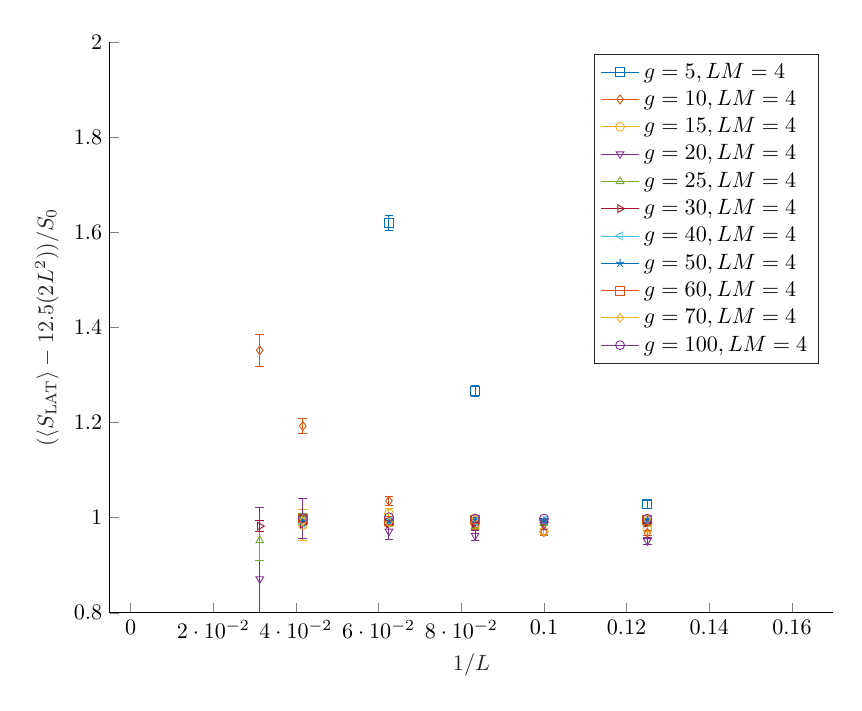
\begin{tikzpicture}[thick,scale=0.8, every node/.style={scale=1}]

\begin{axis}[%
width=4.521in,
height=3.566in,
at={(0.758in,0.481in)},
scale only axis,
xmin=-0.005,
xmax=0.17,
xlabel style={font=\color{white!15!black}},
xlabel={$1/L$},
ymin=0.8,
ymax=2,
ylabel style={font=\color{white!15!black}},
ylabel={$(\langle S_{\rm LAT}\rangle - 12.5 (2L^2)) / S_0$},
axis background/.style={fill=white},
axis x line*=bottom,
axis y line*=left,
legend style={legend cell align=left, align=left, draw=white!15!black}
]
\addplot [color=mycolor1, draw=none, mark=square, mark options={solid, mycolor1}]
 plot [error bars/.cd, y dir = both, y explicit]
 table[row sep=crcr, y error plus index=2, y error minus index=3]{%
0.125	1.02844975915539	0.00809728155090294	0.00809728155090294\\
0.0833333333333333	1.26569076205768	0.0115825506126014	0.0115825506126014\\
0.0625	1.61923442234287	0.0157848401540442	0.0157848401540442\\
};
\addlegendentry{$g =   5, LM = 4$}

\addplot [color=mycolor2, draw=none, mark=diamond, mark options={solid, mycolor2}]
 plot [error bars/.cd, y dir = both, y explicit]
 table[row sep=crcr, y error plus index=2, y error minus index=3]{%
0.125	0.96806787574427	0.00519742685387765	0.00519742685387765\\
0.1	0.969735964925189	0.00720041179644767	0.00720041179644767\\
0.0833333333333333	0.983612026468609	0.00864124458625702	0.00864124458625702\\
0.0625	1.03527725539367	0.00939784943183052	0.00939784943183052\\
0.0416666666666667	1.19278629747492	0.0165788601819162	0.0165788601819162\\
0.03125	1.35203433485177	0.0343204174125818	0.0343204174125818\\
};
\addlegendentry{$g =  10, LM = 4$}

\addplot [color=mycolor3, draw=none, mark=o, mark options={solid, mycolor3}]
 plot [error bars/.cd, y dir = both, y explicit]
 table[row sep=crcr, y error plus index=2, y error minus index=3]{%
0.125	0.976454772326076	0.00509971248010321	0.00509971248010321\\
0.1	0.971386527450655	0.00640208447918485	0.00640208447918485\\
0.0833333333333333	0.98558045714848	0.00745862215350882	0.00745862215350882\\
0.0625	1.00884642593653	0.0112252797635939	0.0112252797635939\\
0.0416666666666667	0.984439479309238	0.0321996500250138	0.0321996500250138\\
};
\addlegendentry{$g =  15, LM = 4$}

\addplot [color=mycolor4, draw=none, mark=triangle, mark options={solid, rotate=180, mycolor4}]
 plot [error bars/.cd, y dir = both, y explicit]
 table[row sep=crcr, y error plus index=2, y error minus index=3]{%
0.125	0.951102706249852	0.00766848632767058	0.00766848632767058\\
0.1	0.985121542789869	0.0100802271800317	0.0100802271800317\\
0.0833333333333333	0.962356250366547	0.00992825266295143	0.00992825266295143\\
0.0625	0.971168678915962	0.0162029467534747	0.0162029467534747\\
0.0416666666666667	0.998610053012655	0.042020762345087	0.042020762345087\\
0.03125	0.871083992279097	0.149866729419579	0.149866729419579\\
};
\addlegendentry{$g =  20, LM = 4$}

\addplot [color=mycolor5, draw=none, mark=triangle, mark options={solid, mycolor5}]
 plot [error bars/.cd, y dir = both, y explicit]
 table[row sep=crcr, y error plus index=2, y error minus index=3]{%
0.125	0.987510825736886	0.00159699494627747	0.00159699494627747\\
0.1	0.988132782200004	0.00203352518234746	0.00203352518234746\\
0.0833333333333333	0.981299920156358	0.00238282598761799	0.00238282598761799\\
0.0625	0.98646713125984	0.00327483306604511	0.00327483306604511\\
0.0416666666666667	0.999172897951517	0.00978122006591181	0.00978122006591181\\
0.03125	0.952063243237262	0.0410593728977441	0.0410593728977441\\
};
\addlegendentry{$g =  25, LM = 4$}

\addplot [color=mycolor6, draw=none, mark=triangle, mark options={solid, rotate=270, mycolor6}]
 plot [error bars/.cd, y dir = both, y explicit]
 table[row sep=crcr, y error plus index=2, y error minus index=3]{%
0.125	0.988784468753521	0.000933097635104395	0.000933097635104395\\
0.1	0.990643288405012	0.00108673358638426	0.00108673358638426\\
0.0833333333333333	0.988959539671448	0.00130199426000922	0.00130199426000922\\
0.0625	0.987499533453164	0.001782432593097	0.001782432593097\\
0.0416666666666667	0.987061272313792	0.00265827834849471	0.00265827834849471\\
0.03125	0.982171340938578	0.0111660837658253	0.0111660837658253\\
0.125	0.989783295437701	0.0011739971308694	0.0011739971308694\\
0.0833333333333333	0.988146411082463	0.0017369108971226	0.0017369108971226\\
0.0625	0.986766549793082	0.00331762148256274	0.00331762148256274\\
};
\addlegendentry{$g =  30, LM = 4$}

\addplot [color=mycolor7, draw=none, mark=triangle, mark options={solid, rotate=90, mycolor7}]
 plot [error bars/.cd, y dir = both, y explicit]
 table[row sep=crcr, y error plus index=2, y error minus index=3]{%
0.125	0.992998337372517	0.000489461336505172	0.000489461336505172\\
0.1	0.993865541206289	0.000662763592751263	0.000662763592751263\\
0.0833333333333333	0.991983139767409	0.000765418769350319	0.000765418769350319\\
0.0625	0.992851350872334	0.000991419188469143	0.000991419188469143\\
0.0416666666666667	0.987723672971182	0.00299190280715426	0.00299190280715426\\
0.125	0.993963368583834	0.00068351027759447	0.00068351027759447\\
0.0833333333333333	0.991694191434016	0.00100733440627698	0.00100733440627698\\
0.0625	0.993384831560734	0.00217268815584469	0.00217268815584469\\
};
\addlegendentry{$g =  40, LM = 4$}

\addplot [color=mycolor1, draw=none, mark=star, mark options={solid, mycolor1}]
 plot [error bars/.cd, y dir = both, y explicit]
 table[row sep=crcr, y error plus index=2, y error minus index=3]{%
0.125	0.995097178409106	0.000433555278524319	0.000433555278524319\\
0.1	0.993856817800818	0.000529171927360768	0.000529171927360768\\
0.0833333333333333	0.995450879040837	0.000688645870715746	0.000688645870715746\\
0.0625	0.993525570173103	0.000913484366298338	0.000913484366298338\\
0.0416666666666667	0.993047671772686	0.00291003050271964	0.00291003050271964\\
0.125	0.995579888702395	0.000627618121342883	0.000627618121342883\\
0.0833333333333333	0.995263988155162	0.000870918552948944	0.000870918552948944\\
0.0625	0.992578285364301	0.00178281419886465	0.00178281419886465\\
};
\addlegendentry{$g =  50, LM = 4$}

\addplot [color=mycolor2, draw=none, mark=square, mark options={solid, mycolor2}]
 plot [error bars/.cd, y dir = both, y explicit]
 table[row sep=crcr, y error plus index=2, y error minus index=3]{%
0.125	0.995504503634062	0.000436946444523767	0.000436946444523767\\
0.0833333333333333	0.996324323300597	0.000941822973121717	0.000941822973121717\\
0.0625	0.993820673080822	0.00241259036636517	0.00241259036636517\\
0.0416666666666667	0.99829132734423	0.00600962750136519	0.00600962750136519\\
};
\addlegendentry{$g =  60, LM = 4$}

\addplot [color=mycolor3, draw=none, mark=diamond, mark options={solid, mycolor3}]
 plot [error bars/.cd, y dir = both, y explicit]
 table[row sep=crcr, y error plus index=2, y error minus index=3]{%
0.125	0.996597282927967	0.000631614829086272	0.000631614829086272\\
0.0833333333333333	0.997903073743863	0.0010094901624273	0.0010094901624273\\
0.0625	0.990123512796802	0.00250711288992565	0.00250711288992565\\
0.0416666666666667	0.992508133415797	0.00978069373328837	0.00978069373328837\\
};
\addlegendentry{$g =  70, LM = 4$}

\addplot [color=mycolor4, draw=none, mark=o, mark options={solid, mycolor4}]
 plot [error bars/.cd, y dir = both, y explicit]
 table[row sep=crcr, y error plus index=2, y error minus index=3]{%
0.125	0.997572913670396	0.000870558555141459	0.000870558555141459\\
0.1	0.998054383392837	0.00106441698953455	0.00106441698953455\\
0.0833333333333333	0.998267159849181	0.00138851590660228	0.00138851590660228\\
0.0625	1.00100206754072	0.0017520197218875	0.0017520197218875\\
0.0416666666666667	0.998936646633082	0.00394692966367991	0.00394692966367991\\
};
\addlegendentry{$g = 100, LM = 4$}

\end{axis}
\end{tikzpicture}%
\caption{Plot of the ratio $\frac{\langle S_{\rm LAT}\rangle -\frac{c}{2}\big(2L^{2}\big)}{S_{0}} \equiv \frac{f'(g)}{4}$, where its coefficient of the divergent contribution $c$ has been fixed to the value $c=15$ and $S_{0}=\frac{1}{2}M^{2}\big(2L^{2}\big)g$. For very large $g$, there is agreement with the continuum prediction $f'(g)=4$ in (\ref{eq: scaling_fct}). For smaller values ($g=10,5$) strong deviations appear.
\label{fig: Slat-c_fix}}
\end{figure}
%
%
\begin{figure}
\centering
% This file was created by matlab2tikz.
%
%The latest updates can be retrieved from
%  http://www.mathworks.com/matlabcentral/fileexchange/22022-matlab2tikz-matlab2tikz
%where you can also make suggestions and rate matlab2tikz.
%
\definecolor{mycolor1}{rgb}{0.00000,0.44700,0.74100}%
\definecolor{mycolor2}{rgb}{0.85000,0.32500,0.09800}%
\definecolor{mycolor3}{rgb}{0.92900,0.69400,0.12500}%
\definecolor{mycolor4}{rgb}{0.49400,0.18400,0.55600}%
\definecolor{mycolor5}{rgb}{0.46600,0.67400,0.18800}%
\definecolor{mycolor6}{rgb}{0.63500,0.07800,0.18400}%
\definecolor{mycolor7}{rgb}{0.30100,0.74500,0.93300}%
%
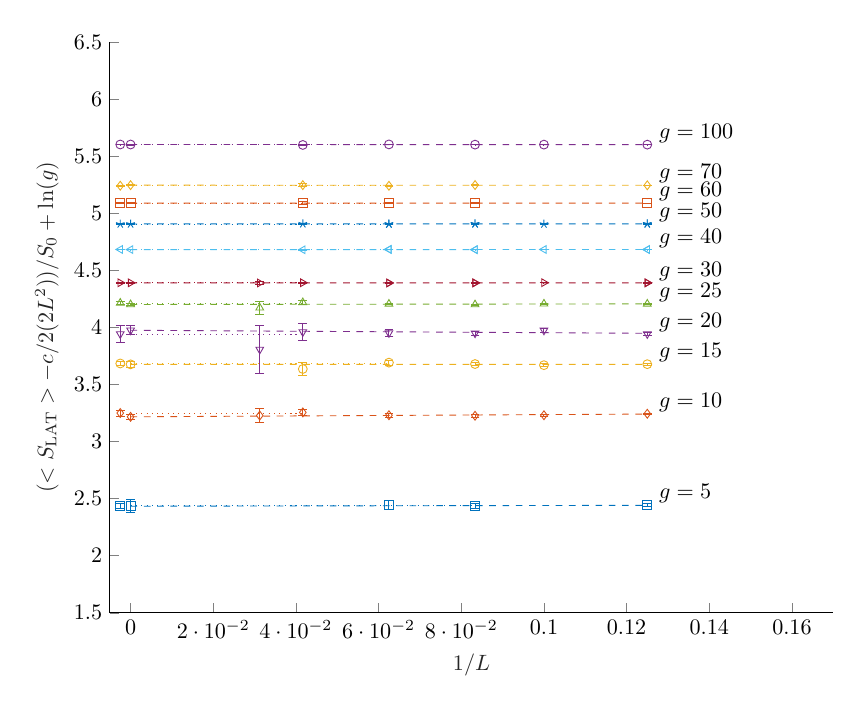
\begin{tikzpicture}[thick,scale=0.8, every node/.style={scale=1}]

\begin{axis}[%
width=4.521in,
height=3.566in,
at={(0.758in,0.481in)},
scale only axis,
xmin=-0.005,
xmax=0.17,
xlabel style={font=\color{white!15!black}},
xlabel={$1/L$},
ymin=1.5,
ymax=6.5,
ylabel style={font=\color{white!15!black}},
ylabel={$(<S_{\rm LAT}> - c/2 (2L^2)) / S_0 + \ln(g)$},
axis background/.style={fill=white},
axis x line*=bottom,
axis y line*=left
]
\addplot [color=mycolor1, dotted, forget plot]
  table[row sep=crcr]{%
0	2.43727316330578\\
0.00125	2.43727316330578\\
0.0025	2.43727316330578\\
0.00375	2.43727316330578\\
0.005	2.43727316330578\\
0.00625	2.43727316330578\\
0.0075	2.43727316330578\\
0.00875	2.43727316330578\\
0.01	2.43727316330578\\
0.01125	2.43727316330578\\
0.0125	2.43727316330578\\
0.01375	2.43727316330578\\
0.015	2.43727316330578\\
0.01625	2.43727316330578\\
0.0175	2.43727316330578\\
0.01875	2.43727316330578\\
0.02	2.43727316330578\\
0.02125	2.43727316330578\\
0.0225	2.43727316330578\\
0.02375	2.43727316330578\\
0.025	2.43727316330578\\
0.02625	2.43727316330578\\
0.0275	2.43727316330578\\
0.02875	2.43727316330578\\
0.03	2.43727316330578\\
0.03125	2.43727316330578\\
0.0325	2.43727316330578\\
0.03375	2.43727316330578\\
0.035	2.43727316330578\\
0.03625	2.43727316330578\\
0.0375	2.43727316330578\\
0.03875	2.43727316330578\\
0.04	2.43727316330578\\
0.04125	2.43727316330578\\
0.0425	2.43727316330578\\
0.04375	2.43727316330578\\
0.045	2.43727316330578\\
0.04625	2.43727316330578\\
0.0475	2.43727316330578\\
0.04875	2.43727316330578\\
0.05	2.43727316330578\\
0.05125	2.43727316330578\\
0.0525	2.43727316330578\\
0.05375	2.43727316330578\\
0.055	2.43727316330578\\
0.05625	2.43727316330578\\
0.0575	2.43727316330578\\
0.05875	2.43727316330578\\
0.06	2.43727316330578\\
0.06125	2.43727316330578\\
0.0625	2.43727316330578\\
0.06375	2.43727316330578\\
0.065	2.43727316330578\\
0.06625	2.43727316330578\\
0.0675	2.43727316330578\\
0.06875	2.43727316330578\\
0.07	2.43727316330578\\
0.07125	2.43727316330578\\
0.0725	2.43727316330578\\
0.07375	2.43727316330578\\
0.075	2.43727316330578\\
0.07625	2.43727316330578\\
0.0775	2.43727316330578\\
0.07875	2.43727316330578\\
0.08	2.43727316330578\\
0.08125	2.43727316330578\\
0.0825	2.43727316330578\\
};
\addplot [color=mycolor1, dashed, forget plot]
  table[row sep=crcr]{%
0	2.43328517943851\\
0.00125	2.43336689492752\\
0.0025	2.43344861041653\\
0.00375	2.43353032590553\\
0.005	2.43361204139454\\
0.00625	2.43369375688355\\
0.0075	2.43377547237255\\
0.00875	2.43385718786156\\
0.01	2.43393890335056\\
0.01125	2.43402061883957\\
0.0125	2.43410233432858\\
0.01375	2.43418404981758\\
0.015	2.43426576530659\\
0.01625	2.4343474807956\\
0.0175	2.4344291962846\\
0.01875	2.43451091177361\\
0.02	2.43459262726261\\
0.02125	2.43467434275162\\
0.0225	2.43475605824063\\
0.02375	2.43483777372963\\
0.025	2.43491948921864\\
0.02625	2.43500120470765\\
0.0275	2.43508292019665\\
0.02875	2.43516463568566\\
0.03	2.43524635117466\\
0.03125	2.43532806666367\\
0.0325	2.43540978215268\\
0.03375	2.43549149764168\\
0.035	2.43557321313069\\
0.03625	2.4356549286197\\
0.0375	2.4357366441087\\
0.03875	2.43581835959771\\
0.04	2.43590007508672\\
0.04125	2.43598179057572\\
0.0425	2.43606350606473\\
0.04375	2.43614522155373\\
0.045	2.43622693704274\\
0.04625	2.43630865253175\\
0.0475	2.43639036802075\\
0.04875	2.43647208350976\\
0.05	2.43655379899877\\
0.05125	2.43663551448777\\
0.0525	2.43671722997678\\
0.05375	2.43679894546578\\
0.055	2.43688066095479\\
0.05625	2.4369623764438\\
0.0575	2.4370440919328\\
0.05875	2.43712580742181\\
0.06	2.43720752291082\\
0.06125	2.43728923839982\\
0.0625	2.43737095388883\\
0.06375	2.43745266937784\\
0.065	2.43753438486684\\
0.06625	2.43761610035585\\
0.0675	2.43769781584485\\
0.06875	2.43777953133386\\
0.07	2.43786124682287\\
0.07125	2.43794296231187\\
0.0725	2.43802467780088\\
0.07375	2.43810639328989\\
0.075	2.43818810877889\\
0.07625	2.4382698242679\\
0.0775	2.4383515397569\\
0.07875	2.43843325524591\\
0.08	2.43851497073492\\
0.08125	2.43859668622392\\
0.0825	2.43867840171293\\
0.08375	2.43876011720194\\
0.085	2.43884183269094\\
0.08625	2.43892354817995\\
0.0875	2.43900526366895\\
0.08875	2.43908697915796\\
0.09	2.43916869464697\\
0.09125	2.43925041013597\\
0.0925	2.43933212562498\\
0.09375	2.43941384111399\\
0.095	2.43949555660299\\
0.09625	2.439577272092\\
0.0975	2.43965898758101\\
0.09875	2.43974070307001\\
0.1	2.43982241855902\\
0.10125	2.43990413404802\\
0.1025	2.43998584953703\\
0.10375	2.44006756502604\\
0.105	2.44014928051504\\
0.10625	2.44023099600405\\
0.1075	2.44031271149306\\
0.10875	2.44039442698206\\
0.11	2.44047614247107\\
0.11125	2.44055785796008\\
0.1125	2.44063957344908\\
0.11375	2.44072128893809\\
0.115	2.44080300442709\\
0.11625	2.4408847199161\\
0.1175	2.44096643540511\\
0.11875	2.44104815089411\\
0.12	2.44112986638312\\
0.12125	2.44121158187213\\
0.1225	2.44129329736113\\
0.12375	2.44137501285014\\
0.125	2.44145672833914\\
};
\addplot [color=mycolor1, draw=none, mark=square, mark options={solid, mycolor1}, forget plot]
 plot [error bars/.cd, y dir = both, y explicit]
 table[row sep=crcr, y error plus index=2, y error minus index=3]{%
0	2.43328517943851	0.0571160600925337	0.0571160600925337\\
-0.0025	2.43727316330578	0.0206422459243649	0.0206422459243649\\
0.125	2.44193553690936	0.0138049762723457	0.0138049762723457\\
0.0833333333333333	2.43423636264366	0.0244248639926938	0.0244248639926938\\
0.0625	2.44486379605648	0.0386156190398151	0.0386156190398151\\
};
\node[right, align=left]
at (axis cs:0.126,2.542) {$g = 5$};
\addplot [color=mycolor2, dotted, forget plot]
  table[row sep=crcr]{%
0	3.24982928552263\\
0.00125	3.24982928552263\\
0.0025	3.24982928552263\\
0.00375	3.24982928552263\\
0.005	3.24982928552263\\
0.00625	3.24982928552263\\
0.0075	3.24982928552263\\
0.00875	3.24982928552263\\
0.01	3.24982928552263\\
0.01125	3.24982928552263\\
0.0125	3.24982928552263\\
0.01375	3.24982928552263\\
0.015	3.24982928552263\\
0.01625	3.24982928552263\\
0.0175	3.24982928552263\\
0.01875	3.24982928552263\\
0.02	3.24982928552263\\
0.02125	3.24982928552263\\
0.0225	3.24982928552263\\
0.02375	3.24982928552263\\
0.025	3.24982928552263\\
0.02625	3.24982928552263\\
0.0275	3.24982928552263\\
0.02875	3.24982928552263\\
0.03	3.24982928552263\\
0.03125	3.24982928552263\\
0.0325	3.24982928552263\\
0.03375	3.24982928552263\\
0.035	3.24982928552263\\
0.03625	3.24982928552263\\
0.0375	3.24982928552263\\
0.03875	3.24982928552263\\
0.04	3.24982928552263\\
0.04125	3.24982928552263\\
};
\addplot [color=mycolor2, dashed, forget plot]
  table[row sep=crcr]{%
0	3.21703525642333\\
0.00125	3.21727601730145\\
0.0025	3.21751677817957\\
0.00375	3.21775753905768\\
0.005	3.2179982999358\\
0.00625	3.21823906081392\\
0.0075	3.21847982169204\\
0.00875	3.21872058257015\\
0.01	3.21896134344827\\
0.01125	3.21920210432639\\
0.0125	3.21944286520451\\
0.01375	3.21968362608263\\
0.015	3.21992438696074\\
0.01625	3.22016514783886\\
0.0175	3.22040590871698\\
0.01875	3.2206466695951\\
0.02	3.22088743047321\\
0.02125	3.22112819135133\\
0.0225	3.22136895222945\\
0.02375	3.22160971310757\\
0.025	3.22185047398568\\
0.02625	3.2220912348638\\
0.0275	3.22233199574192\\
0.02875	3.22257275662004\\
0.03	3.22281351749815\\
0.03125	3.22305427837627\\
0.0325	3.22329503925439\\
0.03375	3.22353580013251\\
0.035	3.22377656101063\\
0.03625	3.22401732188874\\
0.0375	3.22425808276686\\
0.03875	3.22449884364498\\
0.04	3.2247396045231\\
0.04125	3.22498036540121\\
0.0425	3.22522112627933\\
0.04375	3.22546188715745\\
0.045	3.22570264803557\\
0.04625	3.22594340891368\\
0.0475	3.2261841697918\\
0.04875	3.22642493066992\\
0.05	3.22666569154804\\
0.05125	3.22690645242615\\
0.0525	3.22714721330427\\
0.05375	3.22738797418239\\
0.055	3.22762873506051\\
0.05625	3.22786949593862\\
0.0575	3.22811025681674\\
0.05875	3.22835101769486\\
0.06	3.22859177857298\\
0.06125	3.2288325394511\\
0.0625	3.22907330032921\\
0.06375	3.22931406120733\\
0.065	3.22955482208545\\
0.06625	3.22979558296357\\
0.0675	3.23003634384168\\
0.06875	3.2302771047198\\
0.07	3.23051786559792\\
0.07125	3.23075862647604\\
0.0725	3.23099938735415\\
0.07375	3.23124014823227\\
0.075	3.23148090911039\\
0.07625	3.23172166998851\\
0.0775	3.23196243086662\\
0.07875	3.23220319174474\\
0.08	3.23244395262286\\
0.08125	3.23268471350098\\
0.0825	3.23292547437909\\
0.08375	3.23316623525721\\
0.085	3.23340699613533\\
0.08625	3.23364775701345\\
0.0875	3.23388851789157\\
0.08875	3.23412927876968\\
0.09	3.2343700396478\\
0.09125	3.23461080052592\\
0.0925	3.23485156140404\\
0.09375	3.23509232228215\\
0.095	3.23533308316027\\
0.09625	3.23557384403839\\
0.0975	3.23581460491651\\
0.09875	3.23605536579462\\
0.1	3.23629612667274\\
0.10125	3.23653688755086\\
0.1025	3.23677764842898\\
0.10375	3.23701840930709\\
0.105	3.23725917018521\\
0.10625	3.23749993106333\\
0.1075	3.23774069194145\\
0.10875	3.23798145281957\\
0.11	3.23822221369768\\
0.11125	3.2384629745758\\
0.1125	3.23870373545392\\
0.11375	3.23894449633204\\
0.115	3.23918525721015\\
0.11625	3.23942601808827\\
0.1175	3.23966677896639\\
0.11875	3.23990753984451\\
0.12	3.24014830072262\\
0.12125	3.24038906160074\\
0.1225	3.24062982247886\\
0.12375	3.24087058335698\\
0.125	3.24111134423509\\
};
\addplot [color=mycolor2, draw=none, mark=diamond, mark options={solid, mycolor2}, forget plot]
 plot [error bars/.cd, y dir = both, y explicit]
 table[row sep=crcr, y error plus index=2, y error minus index=3]{%
0	3.21703525642333	0.0211018662927336	0.0211018662927336\\
-0.0025	3.24982928552263	0.0269603977359257	0.0269603977359257\\
0.125	3.24400782104094	0.00672638612937152	0.00672638612937152\\
0.1	3.23068801464209	0.00958941066440683	0.00958941066440683\\
0.0833333333333333	3.22624553594453	0.0120814030249214	0.0120814030249214\\
0.0625	3.23128175759823	0.015513686533806	0.015513686533806\\
0.0416666666666667	3.2555650420081	0.0303394947622117	0.0303394947622117\\
0.03125	3.22829706468785	0.0587837658204836	0.0587837658204836\\
};
\node[right, align=left]
at (axis cs:0.126,3.344) {$g = 10$};
\addplot [color=mycolor3, dotted, forget plot]
  table[row sep=crcr]{%
0	3.68443945181043\\
0.00125	3.68443945181043\\
0.0025	3.68443945181043\\
0.00375	3.68443945181043\\
0.005	3.68443945181043\\
0.00625	3.68443945181043\\
0.0075	3.68443945181043\\
0.00875	3.68443945181043\\
0.01	3.68443945181043\\
0.01125	3.68443945181043\\
0.0125	3.68443945181043\\
0.01375	3.68443945181043\\
0.015	3.68443945181043\\
0.01625	3.68443945181043\\
0.0175	3.68443945181043\\
0.01875	3.68443945181043\\
0.02	3.68443945181043\\
0.02125	3.68443945181043\\
0.0225	3.68443945181043\\
0.02375	3.68443945181043\\
0.025	3.68443945181043\\
0.02625	3.68443945181043\\
0.0275	3.68443945181043\\
0.02875	3.68443945181043\\
0.03	3.68443945181043\\
0.03125	3.68443945181043\\
0.0325	3.68443945181043\\
0.03375	3.68443945181043\\
0.035	3.68443945181043\\
0.03625	3.68443945181043\\
0.0375	3.68443945181043\\
0.03875	3.68443945181043\\
0.04	3.68443945181043\\
0.04125	3.68443945181043\\
0.0425	3.68443945181043\\
0.04375	3.68443945181043\\
0.045	3.68443945181043\\
0.04625	3.68443945181043\\
0.0475	3.68443945181043\\
0.04875	3.68443945181043\\
0.05	3.68443945181043\\
0.05125	3.68443945181043\\
0.0525	3.68443945181043\\
0.05375	3.68443945181043\\
0.055	3.68443945181043\\
0.05625	3.68443945181043\\
0.0575	3.68443945181043\\
0.05875	3.68443945181043\\
0.06	3.68443945181043\\
0.06125	3.68443945181043\\
0.0625	3.68443945181043\\
};
\addplot [color=mycolor3, dashed, forget plot]
  table[row sep=crcr]{%
0	3.67668014355213\\
0.00125	3.67667918280858\\
0.0025	3.67667822206503\\
0.00375	3.67667726132148\\
0.005	3.67667630057794\\
0.00625	3.67667533983439\\
0.0075	3.67667437909084\\
0.00875	3.67667341834729\\
0.01	3.67667245760374\\
0.01125	3.67667149686019\\
0.0125	3.67667053611664\\
0.01375	3.67666957537309\\
0.015	3.67666861462954\\
0.01625	3.67666765388599\\
0.0175	3.67666669314244\\
0.01875	3.67666573239889\\
0.02	3.67666477165534\\
0.02125	3.67666381091179\\
0.0225	3.67666285016824\\
0.02375	3.67666188942469\\
0.025	3.67666092868115\\
0.02625	3.6766599679376\\
0.0275	3.67665900719405\\
0.02875	3.6766580464505\\
0.03	3.67665708570695\\
0.03125	3.6766561249634\\
0.0325	3.67665516421985\\
0.03375	3.6766542034763\\
0.035	3.67665324273275\\
0.03625	3.6766522819892\\
0.0375	3.67665132124565\\
0.03875	3.6766503605021\\
0.04	3.67664939975855\\
0.04125	3.676648439015\\
0.0425	3.67664747827145\\
0.04375	3.67664651752791\\
0.045	3.67664555678436\\
0.04625	3.67664459604081\\
0.0475	3.67664363529726\\
0.04875	3.67664267455371\\
0.05	3.67664171381016\\
0.05125	3.67664075306661\\
0.0525	3.67663979232306\\
0.05375	3.67663883157951\\
0.055	3.67663787083596\\
0.05625	3.67663691009241\\
0.0575	3.67663594934886\\
0.05875	3.67663498860531\\
0.06	3.67663402786176\\
0.06125	3.67663306711821\\
0.0625	3.67663210637467\\
0.06375	3.67663114563112\\
0.065	3.67663018488757\\
0.06625	3.67662922414402\\
0.0675	3.67662826340047\\
0.06875	3.67662730265692\\
0.07	3.67662634191337\\
0.07125	3.67662538116982\\
0.0725	3.67662442042627\\
0.07375	3.67662345968272\\
0.075	3.67662249893917\\
0.07625	3.67662153819562\\
0.0775	3.67662057745207\\
0.07875	3.67661961670852\\
0.08	3.67661865596497\\
0.08125	3.67661769522143\\
0.0825	3.67661673447788\\
0.08375	3.67661577373433\\
0.085	3.67661481299078\\
0.08625	3.67661385224723\\
0.0875	3.67661289150368\\
0.08875	3.67661193076013\\
0.09	3.67661097001658\\
0.09125	3.67661000927303\\
0.0925	3.67660904852948\\
0.09375	3.67660808778593\\
0.095	3.67660712704238\\
0.09625	3.67660616629883\\
0.0975	3.67660520555528\\
0.09875	3.67660424481173\\
0.1	3.67660328406819\\
0.10125	3.67660232332464\\
0.1025	3.67660136258109\\
0.10375	3.67660040183754\\
0.105	3.67659944109399\\
0.10625	3.67659848035044\\
0.1075	3.67659751960689\\
0.10875	3.67659655886334\\
0.11	3.67659559811979\\
0.11125	3.67659463737624\\
0.1125	3.67659367663269\\
0.11375	3.67659271588914\\
0.115	3.67659175514559\\
0.11625	3.67659079440204\\
0.1175	3.67658983365849\\
0.11875	3.67658887291495\\
0.12	3.6765879121714\\
0.12125	3.67658695142785\\
0.1225	3.6765859906843\\
0.12375	3.67658502994075\\
0.125	3.6765840691972\\
};
\addplot [color=mycolor3, draw=none, mark=o, mark options={solid, mycolor3}, forget plot]
 plot [error bars/.cd, y dir = both, y explicit]
 table[row sep=crcr, y error plus index=2, y error minus index=3]{%
0	3.67668014355213	0.0298127620723799	0.0298127620723799\\
-0.0025	3.68443945181043	0.0213018362804732	0.0213018362804732\\
0.125	3.67824291574353	0.00801266770548511	0.00801266770548511\\
0.1	3.66965226342043	0.0109535770188441	0.0109535770188441\\
0.0833333333333333	3.67954102817819	0.0140127715417011	0.0140127715417011\\
0.0625	3.69184839629971	0.0228771006651215	0.0228771006651215\\
0.0416666666666667	3.63613115673994	0.0584162491507788	0.0584162491507788\\
};
\node[right, align=left]
at (axis cs:0.126,3.778) {$g = 15$};
\addplot [color=mycolor4, dotted, forget plot]
  table[row sep=crcr]{%
0	3.94321711284596\\
0.00125	3.94321711284596\\
0.0025	3.94321711284596\\
0.00375	3.94321711284596\\
0.005	3.94321711284596\\
0.00625	3.94321711284596\\
0.0075	3.94321711284596\\
0.00875	3.94321711284596\\
0.01	3.94321711284596\\
0.01125	3.94321711284596\\
0.0125	3.94321711284596\\
0.01375	3.94321711284596\\
0.015	3.94321711284596\\
0.01625	3.94321711284596\\
0.0175	3.94321711284596\\
0.01875	3.94321711284596\\
0.02	3.94321711284596\\
0.02125	3.94321711284596\\
0.0225	3.94321711284596\\
0.02375	3.94321711284596\\
0.025	3.94321711284596\\
0.02625	3.94321711284596\\
0.0275	3.94321711284596\\
0.02875	3.94321711284596\\
0.03	3.94321711284596\\
0.03125	3.94321711284596\\
0.0325	3.94321711284596\\
0.03375	3.94321711284596\\
0.035	3.94321711284596\\
0.03625	3.94321711284596\\
0.0375	3.94321711284596\\
0.03875	3.94321711284596\\
0.04	3.94321711284596\\
0.04125	3.94321711284596\\
};
\addplot [color=mycolor4, dashed, forget plot]
  table[row sep=crcr]{%
0	3.97550737751373\\
0.00125	3.975240446593\\
0.0025	3.97497351567227\\
0.00375	3.97470658475154\\
0.005	3.97443965383081\\
0.00625	3.97417272291008\\
0.0075	3.97390579198935\\
0.00875	3.97363886106862\\
0.01	3.97337193014789\\
0.01125	3.97310499922716\\
0.0125	3.97283806830643\\
0.01375	3.9725711373857\\
0.015	3.97230420646497\\
0.01625	3.97203727554424\\
0.0175	3.97177034462351\\
0.01875	3.97150341370278\\
0.02	3.97123648278205\\
0.02125	3.97096955186132\\
0.0225	3.97070262094059\\
0.02375	3.97043569001986\\
0.025	3.97016875909913\\
0.02625	3.9699018281784\\
0.0275	3.96963489725767\\
0.02875	3.96936796633694\\
0.03	3.96910103541621\\
0.03125	3.96883410449548\\
0.0325	3.96856717357475\\
0.03375	3.96830024265402\\
0.035	3.96803331173329\\
0.03625	3.96776638081256\\
0.0375	3.96749944989183\\
0.03875	3.9672325189711\\
0.04	3.96696558805036\\
0.04125	3.96669865712963\\
0.0425	3.9664317262089\\
0.04375	3.96616479528817\\
0.045	3.96589786436744\\
0.04625	3.96563093344671\\
0.0475	3.96536400252598\\
0.04875	3.96509707160525\\
0.05	3.96483014068452\\
0.05125	3.96456320976379\\
0.0525	3.96429627884306\\
0.05375	3.96402934792233\\
0.055	3.9637624170016\\
0.05625	3.96349548608087\\
0.0575	3.96322855516014\\
0.05875	3.96296162423941\\
0.06	3.96269469331868\\
0.06125	3.96242776239795\\
0.0625	3.96216083147722\\
0.06375	3.96189390055649\\
0.065	3.96162696963576\\
0.06625	3.96136003871503\\
0.0675	3.9610931077943\\
0.06875	3.96082617687357\\
0.07	3.96055924595284\\
0.07125	3.96029231503211\\
0.0725	3.96002538411138\\
0.07375	3.95975845319065\\
0.075	3.95949152226992\\
0.07625	3.95922459134919\\
0.0775	3.95895766042846\\
0.07875	3.95869072950773\\
0.08	3.958423798587\\
0.08125	3.95815686766626\\
0.0825	3.95788993674553\\
0.08375	3.9576230058248\\
0.085	3.95735607490407\\
0.08625	3.95708914398334\\
0.0875	3.95682221306261\\
0.08875	3.95655528214188\\
0.09	3.95628835122115\\
0.09125	3.95602142030042\\
0.0925	3.95575448937969\\
0.09375	3.95548755845896\\
0.095	3.95522062753823\\
0.09625	3.9549536966175\\
0.0975	3.95468676569677\\
0.09875	3.95441983477604\\
0.1	3.95415290385531\\
0.10125	3.95388597293458\\
0.1025	3.95361904201385\\
0.10375	3.95335211109312\\
0.105	3.95308518017239\\
0.10625	3.95281824925166\\
0.1075	3.95255131833093\\
0.10875	3.9522843874102\\
0.11	3.95201745648947\\
0.11125	3.95175052556874\\
0.1125	3.95148359464801\\
0.11375	3.95121666372728\\
0.115	3.95094973280655\\
0.11625	3.95068280188582\\
0.1175	3.95041587096509\\
0.11875	3.95014894004436\\
0.12	3.94988200912363\\
0.12125	3.9496150782029\\
0.1225	3.94934814728216\\
0.12375	3.94908121636143\\
0.125	3.9488142854407\\
};
\addplot [color=mycolor4, draw=none, mark=triangle, mark options={solid, rotate=180, mycolor4}, forget plot]
 plot [error bars/.cd, y dir = both, y explicit]
 table[row sep=crcr, y error plus index=2, y error minus index=3]{%
0	3.97550737751373	0.0402815193782696	0.0402815193782696\\
-0.0025	3.94321711284596	0.0714662201770275	0.0714662201770275\\
0.125	3.94312481223356	0.0114429057134635	0.0114429057134635\\
0.1	3.9750566795153	0.0159777574703331	0.0159777574703331\\
0.0833333333333333	3.94974064672045	0.0184206964508344	0.0184206964508344\\
0.0625	3.95206028218883	0.0313006242966464	0.0313006242966464\\
0.0416666666666667	3.96095081576279	0.0759905395348056	0.0759905395348056\\
0.03125	3.80745358470859	0.210257439592266	0.210257439592266\\
};
\node[right, align=left]
at (axis cs:0.126,4.043) {$g = 20$};
\addplot [color=mycolor5, dotted, forget plot]
  table[row sep=crcr]{%
0	4.21484914832195\\
0.00125	4.21484914832195\\
0.0025	4.21484914832195\\
0.00375	4.21484914832195\\
0.005	4.21484914832195\\
0.00625	4.21484914832195\\
0.0075	4.21484914832195\\
0.00875	4.21484914832195\\
0.01	4.21484914832195\\
0.01125	4.21484914832195\\
0.0125	4.21484914832195\\
0.01375	4.21484914832195\\
0.015	4.21484914832195\\
0.01625	4.21484914832195\\
0.0175	4.21484914832195\\
0.01875	4.21484914832195\\
0.02	4.21484914832195\\
0.02125	4.21484914832195\\
0.0225	4.21484914832195\\
0.02375	4.21484914832195\\
0.025	4.21484914832195\\
0.02625	4.21484914832195\\
0.0275	4.21484914832195\\
0.02875	4.21484914832195\\
0.03	4.21484914832195\\
0.03125	4.21484914832195\\
0.0325	4.21484914832195\\
0.03375	4.21484914832195\\
0.035	4.21484914832195\\
0.03625	4.21484914832195\\
0.0375	4.21484914832195\\
0.03875	4.21484914832195\\
0.04	4.21484914832195\\
0.04125	4.21484914832195\\
};
\addplot [color=mycolor5, dashed, forget plot]
  table[row sep=crcr]{%
0	4.20140477798615\\
0.00125	4.20145573462367\\
0.0025	4.2015066912612\\
0.00375	4.20155764789873\\
0.005	4.20160860453626\\
0.00625	4.20165956117379\\
0.0075	4.20171051781131\\
0.00875	4.20176147444884\\
0.01	4.20181243108637\\
0.01125	4.2018633877239\\
0.0125	4.20191434436143\\
0.01375	4.20196530099895\\
0.015	4.20201625763648\\
0.01625	4.20206721427401\\
0.0175	4.20211817091154\\
0.01875	4.20216912754906\\
0.02	4.20222008418659\\
0.02125	4.20227104082412\\
0.0225	4.20232199746165\\
0.02375	4.20237295409918\\
0.025	4.2024239107367\\
0.02625	4.20247486737423\\
0.0275	4.20252582401176\\
0.02875	4.20257678064929\\
0.03	4.20262773728682\\
0.03125	4.20267869392434\\
0.0325	4.20272965056187\\
0.03375	4.2027806071994\\
0.035	4.20283156383693\\
0.03625	4.20288252047445\\
0.0375	4.20293347711198\\
0.03875	4.20298443374951\\
0.04	4.20303539038704\\
0.04125	4.20308634702457\\
0.0425	4.20313730366209\\
0.04375	4.20318826029962\\
0.045	4.20323921693715\\
0.04625	4.20329017357468\\
0.0475	4.20334113021221\\
0.04875	4.20339208684973\\
0.05	4.20344304348726\\
0.05125	4.20349400012479\\
0.0525	4.20354495676232\\
0.05375	4.20359591339985\\
0.055	4.20364687003737\\
0.05625	4.2036978266749\\
0.0575	4.20374878331243\\
0.05875	4.20379973994996\\
0.06	4.20385069658748\\
0.06125	4.20390165322501\\
0.0625	4.20395260986254\\
0.06375	4.20400356650007\\
0.065	4.2040545231376\\
0.06625	4.20410547977512\\
0.0675	4.20415643641265\\
0.06875	4.20420739305018\\
0.07	4.20425834968771\\
0.07125	4.20430930632524\\
0.0725	4.20436026296276\\
0.07375	4.20441121960029\\
0.075	4.20446217623782\\
0.07625	4.20451313287535\\
0.0775	4.20456408951288\\
0.07875	4.2046150461504\\
0.08	4.20466600278793\\
0.08125	4.20471695942546\\
0.0825	4.20476791606299\\
0.08375	4.20481887270051\\
0.085	4.20486982933804\\
0.08625	4.20492078597557\\
0.0875	4.2049717426131\\
0.08875	4.20502269925063\\
0.09	4.20507365588815\\
0.09125	4.20512461252568\\
0.0925	4.20517556916321\\
0.09375	4.20522652580074\\
0.095	4.20527748243827\\
0.09625	4.20532843907579\\
0.0975	4.20537939571332\\
0.09875	4.20543035235085\\
0.1	4.20548130898838\\
0.10125	4.20553226562591\\
0.1025	4.20558322226343\\
0.10375	4.20563417890096\\
0.105	4.20568513553849\\
0.10625	4.20573609217602\\
0.1075	4.20578704881355\\
0.10875	4.20583800545107\\
0.11	4.2058889620886\\
0.11125	4.20593991872613\\
0.1125	4.20599087536366\\
0.11375	4.20604183200119\\
0.115	4.20609278863871\\
0.11625	4.20614374527624\\
0.1175	4.20619470191377\\
0.11875	4.2062456585513\\
0.12	4.20629661518882\\
0.12125	4.20634757182635\\
0.1225	4.20639852846388\\
0.12375	4.20644948510141\\
0.125	4.20650044173894\\
};
\addplot [color=mycolor5, draw=none, mark=triangle, mark options={solid, mycolor5}, forget plot]
 plot [error bars/.cd, y dir = both, y explicit]
 table[row sep=crcr, y error plus index=2, y error minus index=3]{%
0	4.20140477798615	0.0088567602625571	0.0088567602625571\\
-0.0025	4.21484914832195	0.0165352187648858	0.0165352187648858\\
0.125	4.20650421676597	0.00243825407478115	0.00243825407478115\\
0.1	4.20719230419459	0.00334799257063447	0.00334799257063447\\
0.0833333333333333	4.20044026889185	0.00427565906460794	0.00427565906460794\\
0.0625	4.20581322077159	0.00663986958005985	0.00663986958005985\\
0.0416666666666667	4.21910681835235	0.0173525528281516	0.0173525528281516\\
0.03125	4.17282012667966	0.0545195189538031	0.0545195189538031\\
};
\node[right, align=left]
at (axis cs:0.126,4.307) {$g = 25$};
\addplot [color=mycolor6, dotted, forget plot]
  table[row sep=crcr]{%
0	4.39176690611519\\
0.00125	4.39176690611519\\
0.0025	4.39176690611519\\
0.00375	4.39176690611519\\
0.005	4.39176690611519\\
0.00625	4.39176690611519\\
0.0075	4.39176690611519\\
0.00875	4.39176690611519\\
0.01	4.39176690611519\\
0.01125	4.39176690611519\\
0.0125	4.39176690611519\\
0.01375	4.39176690611519\\
0.015	4.39176690611519\\
0.01625	4.39176690611519\\
0.0175	4.39176690611519\\
0.01875	4.39176690611519\\
0.02	4.39176690611519\\
0.02125	4.39176690611519\\
0.0225	4.39176690611519\\
0.02375	4.39176690611519\\
0.025	4.39176690611519\\
0.02625	4.39176690611519\\
0.0275	4.39176690611519\\
0.02875	4.39176690611519\\
0.03	4.39176690611519\\
0.03125	4.39176690611519\\
0.0325	4.39176690611519\\
0.03375	4.39176690611519\\
0.035	4.39176690611519\\
0.03625	4.39176690611519\\
0.0375	4.39176690611519\\
0.03875	4.39176690611519\\
0.04	4.39176690611519\\
0.04125	4.39176690611519\\
};
\addplot [color=mycolor6, dashed, forget plot]
  table[row sep=crcr]{%
0	4.39119051787316\\
0.00125	4.39118925615299\\
0.0025	4.39118799443281\\
0.00375	4.39118673271264\\
0.005	4.39118547099247\\
0.00625	4.39118420927229\\
0.0075	4.39118294755212\\
0.00875	4.39118168583195\\
0.01	4.39118042411177\\
0.01125	4.3911791623916\\
0.0125	4.39117790067142\\
0.01375	4.39117663895125\\
0.015	4.39117537723108\\
0.01625	4.3911741155109\\
0.0175	4.39117285379073\\
0.01875	4.39117159207056\\
0.02	4.39117033035038\\
0.02125	4.39116906863021\\
0.0225	4.39116780691003\\
0.02375	4.39116654518986\\
0.025	4.39116528346969\\
0.02625	4.39116402174951\\
0.0275	4.39116276002934\\
0.02875	4.39116149830916\\
0.03	4.39116023658899\\
0.03125	4.39115897486882\\
0.0325	4.39115771314864\\
0.03375	4.39115645142847\\
0.035	4.3911551897083\\
0.03625	4.39115392798812\\
0.0375	4.39115266626795\\
0.03875	4.39115140454777\\
0.04	4.3911501428276\\
0.04125	4.39114888110743\\
0.0425	4.39114761938725\\
0.04375	4.39114635766708\\
0.045	4.39114509594691\\
0.04625	4.39114383422673\\
0.0475	4.39114257250656\\
0.04875	4.39114131078639\\
0.05	4.39114004906621\\
0.05125	4.39113878734604\\
0.0525	4.39113752562586\\
0.05375	4.39113626390569\\
0.055	4.39113500218552\\
0.05625	4.39113374046534\\
0.0575	4.39113247874517\\
0.05875	4.39113121702499\\
0.06	4.39112995530482\\
0.06125	4.39112869358465\\
0.0625	4.39112743186447\\
0.06375	4.3911261701443\\
0.065	4.39112490842413\\
0.06625	4.39112364670395\\
0.0675	4.39112238498378\\
0.06875	4.3911211232636\\
0.07	4.39111986154343\\
0.07125	4.39111859982326\\
0.0725	4.39111733810308\\
0.07375	4.39111607638291\\
0.075	4.39111481466274\\
0.07625	4.39111355294256\\
0.0775	4.39111229122239\\
0.07875	4.39111102950221\\
0.08	4.39110976778204\\
0.08125	4.39110850606187\\
0.0825	4.39110724434169\\
0.08375	4.39110598262152\\
0.085	4.39110472090135\\
0.08625	4.39110345918117\\
0.0875	4.391102197461\\
0.08875	4.39110093574083\\
0.09	4.39109967402065\\
0.09125	4.39109841230048\\
0.0925	4.3910971505803\\
0.09375	4.39109588886013\\
0.095	4.39109462713996\\
0.09625	4.39109336541978\\
0.0975	4.39109210369961\\
0.09875	4.39109084197943\\
0.1	4.39108958025926\\
0.10125	4.39108831853909\\
0.1025	4.39108705681891\\
0.10375	4.39108579509874\\
0.105	4.39108453337857\\
0.10625	4.39108327165839\\
0.1075	4.39108200993822\\
0.10875	4.39108074821804\\
0.11	4.39107948649787\\
0.11125	4.3910782247777\\
0.1125	4.39107696305752\\
0.11375	4.39107570133735\\
0.115	4.39107443961718\\
0.11625	4.391073177897\\
0.1175	4.39107191617683\\
0.11875	4.39107065445665\\
0.12	4.39106939273648\\
0.12125	4.39106813101631\\
0.1225	4.39106686929613\\
0.12375	4.39106560757596\\
0.125	4.39106434585579\\
};
\addplot [color=mycolor6, draw=none, mark=triangle, mark options={solid, rotate=270, mycolor6}, forget plot]
 plot [error bars/.cd, y dir = both, y explicit]
 table[row sep=crcr, y error plus index=2, y error minus index=3]{%
0	4.39119051787316	0.00319622894973694	0.00319622894973694\\
-0.0025	4.39176690611519	0.00496573248160645	0.00496573248160645\\
0.125	4.39039383231555	0.00121916255472723	0.00121916255472723\\
0.1	4.39248439178572	0.00153371002329494	0.00153371002329494\\
0.0833333333333333	4.39108388062685	0.00194564034203353	0.00194564034203353\\
0.0625	4.39034484271481	0.00292669227158835	0.00292669227158835\\
0.0416666666666667	4.39196649137141	0.005232862831067	0.005232862831067\\
0.03125	4.38996043299868	0.0157431224797907	0.0157431224797907\\
0.125	4.39139265899973	0.00146006205049224	0.00146006205049224\\
0.0833333333333333	4.39027075203787	0.00238055697914691	0.00238055697914691\\
0.0625	4.38961185905472	0.00446188116105409	0.00446188116105409\\
};
\node[right, align=left]
at (axis cs:0.126,4.49) {$g = 30$};
\addplot [color=mycolor7, dotted, forget plot]
  table[row sep=crcr]{%
0	4.68352467442952\\
0.00125	4.68352467442952\\
0.0025	4.68352467442952\\
0.00375	4.68352467442952\\
0.005	4.68352467442952\\
0.00625	4.68352467442952\\
0.0075	4.68352467442952\\
0.00875	4.68352467442952\\
0.01	4.68352467442952\\
0.01125	4.68352467442952\\
0.0125	4.68352467442952\\
0.01375	4.68352467442952\\
0.015	4.68352467442952\\
0.01625	4.68352467442952\\
0.0175	4.68352467442952\\
0.01875	4.68352467442952\\
0.02	4.68352467442952\\
0.02125	4.68352467442952\\
0.0225	4.68352467442952\\
0.02375	4.68352467442952\\
0.025	4.68352467442952\\
0.02625	4.68352467442952\\
0.0275	4.68352467442952\\
0.02875	4.68352467442952\\
0.03	4.68352467442952\\
0.03125	4.68352467442952\\
0.0325	4.68352467442952\\
0.03375	4.68352467442952\\
0.035	4.68352467442952\\
0.03625	4.68352467442952\\
0.0375	4.68352467442952\\
0.03875	4.68352467442952\\
0.04	4.68352467442952\\
0.04125	4.68352467442952\\
0.0425	4.68352467442952\\
0.04375	4.68352467442952\\
0.045	4.68352467442952\\
0.04625	4.68352467442952\\
0.0475	4.68352467442952\\
0.04875	4.68352467442952\\
0.05	4.68352467442952\\
0.05125	4.68352467442952\\
0.0525	4.68352467442952\\
0.05375	4.68352467442952\\
0.055	4.68352467442952\\
0.05625	4.68352467442952\\
0.0575	4.68352467442952\\
0.05875	4.68352467442952\\
0.06	4.68352467442952\\
0.06125	4.68352467442952\\
0.0625	4.68352467442952\\
};
\addplot [color=mycolor7, dashed, forget plot]
  table[row sep=crcr]{%
0	4.68258775733734\\
0.00125	4.68258962927052\\
0.0025	4.68259150120369\\
0.00375	4.68259337313687\\
0.005	4.68259524507004\\
0.00625	4.68259711700322\\
0.0075	4.68259898893639\\
0.00875	4.68260086086957\\
0.01	4.68260273280275\\
0.01125	4.68260460473592\\
0.0125	4.6826064766691\\
0.01375	4.68260834860227\\
0.015	4.68261022053545\\
0.01625	4.68261209246863\\
0.0175	4.6826139644018\\
0.01875	4.68261583633498\\
0.02	4.68261770826815\\
0.02125	4.68261958020133\\
0.0225	4.68262145213451\\
0.02375	4.68262332406768\\
0.025	4.68262519600086\\
0.02625	4.68262706793403\\
0.0275	4.68262893986721\\
0.02875	4.68263081180038\\
0.03	4.68263268373356\\
0.03125	4.68263455566674\\
0.0325	4.68263642759991\\
0.03375	4.68263829953309\\
0.035	4.68264017146626\\
0.03625	4.68264204339944\\
0.0375	4.68264391533261\\
0.03875	4.68264578726579\\
0.04	4.68264765919897\\
0.04125	4.68264953113214\\
0.0425	4.68265140306532\\
0.04375	4.68265327499849\\
0.045	4.68265514693167\\
0.04625	4.68265701886485\\
0.0475	4.68265889079802\\
0.04875	4.6826607627312\\
0.05	4.68266263466437\\
0.05125	4.68266450659755\\
0.0525	4.68266637853072\\
0.05375	4.6826682504639\\
0.055	4.68267012239708\\
0.05625	4.68267199433025\\
0.0575	4.68267386626343\\
0.05875	4.6826757381966\\
0.06	4.68267761012978\\
0.06125	4.68267948206296\\
0.0625	4.68268135399613\\
0.06375	4.68268322592931\\
0.065	4.68268509786248\\
0.06625	4.68268696979566\\
0.0675	4.68268884172883\\
0.06875	4.68269071366201\\
0.07	4.68269258559519\\
0.07125	4.68269445752836\\
0.0725	4.68269632946154\\
0.07375	4.68269820139471\\
0.075	4.68270007332789\\
0.07625	4.68270194526107\\
0.0775	4.68270381719424\\
0.07875	4.68270568912742\\
0.08	4.68270756106059\\
0.08125	4.68270943299377\\
0.0825	4.68271130492694\\
0.08375	4.68271317686012\\
0.085	4.6827150487933\\
0.08625	4.68271692072647\\
0.0875	4.68271879265965\\
0.08875	4.68272066459282\\
0.09	4.682722536526\\
0.09125	4.68272440845918\\
0.0925	4.68272628039235\\
0.09375	4.68272815232553\\
0.095	4.6827300242587\\
0.09625	4.68273189619188\\
0.0975	4.68273376812505\\
0.09875	4.68273564005823\\
0.1	4.68273751199141\\
0.10125	4.68273938392458\\
0.1025	4.68274125585776\\
0.10375	4.68274312779093\\
0.105	4.68274499972411\\
0.10625	4.68274687165729\\
0.1075	4.68274874359046\\
0.10875	4.68275061552364\\
0.11	4.68275248745681\\
0.11125	4.68275435938999\\
0.1125	4.68275623132316\\
0.11375	4.68275810325634\\
0.115	4.68275997518952\\
0.11625	4.68276184712269\\
0.1175	4.68276371905587\\
0.11875	4.68276559098904\\
0.12	4.68276746292222\\
0.12125	4.6827693348554\\
0.1225	4.68277120678857\\
0.12375	4.68277307872175\\
0.125	4.68277495065492\\
};
\addplot [color=mycolor7, draw=none, mark=triangle, mark options={solid, rotate=90, mycolor7}, forget plot]
 plot [error bars/.cd, y dir = both, y explicit]
 table[row sep=crcr, y error plus index=2, y error minus index=3]{%
0	4.68258775733734	0.00224141252829221	0.00224141252829221\\
-0.0025	4.68352467442952	0.00159689894833432	0.00159689894833432\\
0.125	4.68235633282895	0.000736428692764701	0.000736428692764701\\
0.1	4.68349271616788	0.00104865008690678	0.00104865008690678\\
0.0833333333333333	4.68193931192351	0.00132109533204779	0.00132109533204779\\
0.0625	4.68364497035627	0.00197928861350726	0.00197928861350726\\
0.0416666666666667	4.68090999951217	0.00521460919130653	0.00521460919130653\\
0.125	4.68332136404027	0.000930477633853999	0.000930477633853999\\
0.0833333333333333	4.68165036359011	0.00156301096897446	0.00156301096897446\\
0.0625	4.68417845104467	0.0031605575808828	0.0031605575808828\\
};
\node[right, align=left]
at (axis cs:0.126,4.782) {$g = 40$};
\addplot [color=mycolor1, dotted, forget plot]
  table[row sep=crcr]{%
0	4.90697440662945\\
0.00125	4.90697440662945\\
0.0025	4.90697440662945\\
0.00375	4.90697440662945\\
0.005	4.90697440662945\\
0.00625	4.90697440662945\\
0.0075	4.90697440662945\\
0.00875	4.90697440662945\\
0.01	4.90697440662945\\
0.01125	4.90697440662945\\
0.0125	4.90697440662945\\
0.01375	4.90697440662945\\
0.015	4.90697440662945\\
0.01625	4.90697440662945\\
0.0175	4.90697440662945\\
0.01875	4.90697440662945\\
0.02	4.90697440662945\\
0.02125	4.90697440662945\\
0.0225	4.90697440662945\\
0.02375	4.90697440662945\\
0.025	4.90697440662945\\
0.02625	4.90697440662945\\
0.0275	4.90697440662945\\
0.02875	4.90697440662945\\
0.03	4.90697440662945\\
0.03125	4.90697440662945\\
0.0325	4.90697440662945\\
0.03375	4.90697440662945\\
0.035	4.90697440662945\\
0.03625	4.90697440662945\\
0.0375	4.90697440662945\\
0.03875	4.90697440662945\\
0.04	4.90697440662945\\
0.04125	4.90697440662945\\
0.0425	4.90697440662945\\
0.04375	4.90697440662945\\
0.045	4.90697440662945\\
0.04625	4.90697440662945\\
0.0475	4.90697440662945\\
0.04875	4.90697440662945\\
0.05	4.90697440662945\\
0.05125	4.90697440662945\\
0.0525	4.90697440662945\\
0.05375	4.90697440662945\\
0.055	4.90697440662945\\
0.05625	4.90697440662945\\
0.0575	4.90697440662945\\
0.05875	4.90697440662945\\
0.06	4.90697440662945\\
0.06125	4.90697440662945\\
0.0625	4.90697440662945\\
};
\addplot [color=mycolor1, dashed, forget plot]
  table[row sep=crcr]{%
0	4.90717147042587\\
0.00125	4.90717548294833\\
0.0025	4.90717949547079\\
0.00375	4.90718350799325\\
0.005	4.90718752051572\\
0.00625	4.90719153303818\\
0.0075	4.90719554556064\\
0.00875	4.90719955808311\\
0.01	4.90720357060557\\
0.01125	4.90720758312803\\
0.0125	4.90721159565049\\
0.01375	4.90721560817296\\
0.015	4.90721962069542\\
0.01625	4.90722363321788\\
0.0175	4.90722764574034\\
0.01875	4.90723165826281\\
0.02	4.90723567078527\\
0.02125	4.90723968330773\\
0.0225	4.90724369583019\\
0.02375	4.90724770835266\\
0.025	4.90725172087512\\
0.02625	4.90725573339758\\
0.0275	4.90725974592004\\
0.02875	4.90726375844251\\
0.03	4.90726777096497\\
0.03125	4.90727178348743\\
0.0325	4.9072757960099\\
0.03375	4.90727980853236\\
0.035	4.90728382105482\\
0.03625	4.90728783357728\\
0.0375	4.90729184609975\\
0.03875	4.90729585862221\\
0.04	4.90729987114467\\
0.04125	4.90730388366713\\
0.0425	4.9073078961896\\
0.04375	4.90731190871206\\
0.045	4.90731592123452\\
0.04625	4.90731993375698\\
0.0475	4.90732394627945\\
0.04875	4.90732795880191\\
0.05	4.90733197132437\\
0.05125	4.90733598384683\\
0.0525	4.9073399963693\\
0.05375	4.90734400889176\\
0.055	4.90734802141422\\
0.05625	4.90735203393669\\
0.0575	4.90735604645915\\
0.05875	4.90736005898161\\
0.06	4.90736407150407\\
0.06125	4.90736808402654\\
0.0625	4.907372096549\\
0.06375	4.90737610907146\\
0.065	4.90738012159392\\
0.06625	4.90738413411639\\
0.0675	4.90738814663885\\
0.06875	4.90739215916131\\
0.07	4.90739617168378\\
0.07125	4.90740018420624\\
0.0725	4.9074041967287\\
0.07375	4.90740820925116\\
0.075	4.90741222177363\\
0.07625	4.90741623429609\\
0.0775	4.90742024681855\\
0.07875	4.90742425934101\\
0.08	4.90742827186348\\
0.08125	4.90743228438594\\
0.0825	4.9074362969084\\
0.08375	4.90744030943086\\
0.085	4.90744432195333\\
0.08625	4.90744833447579\\
0.0875	4.90745234699825\\
0.08875	4.90745635952071\\
0.09	4.90746037204318\\
0.09125	4.90746438456564\\
0.0925	4.9074683970881\\
0.09375	4.90747240961056\\
0.095	4.90747642213303\\
0.09625	4.90748043465549\\
0.0975	4.90748444717795\\
0.09875	4.90748845970042\\
0.1	4.90749247222288\\
0.10125	4.90749648474534\\
0.1025	4.9075004972678\\
0.10375	4.90750450979027\\
0.105	4.90750852231273\\
0.10625	4.90751253483519\\
0.1075	4.90751654735765\\
0.10875	4.90752055988012\\
0.11	4.90752457240258\\
0.11125	4.90752858492504\\
0.1125	4.9075325974475\\
0.11375	4.90753660996997\\
0.115	4.90754062249243\\
0.11625	4.90754463501489\\
0.1175	4.90754864753735\\
0.11875	4.90755266005982\\
0.12	4.90755667258228\\
0.12125	4.90756068510474\\
0.1225	4.90756469762721\\
0.12375	4.90756871014967\\
0.125	4.90757272267213\\
};
\addplot [color=mycolor1, draw=none, mark=star, mark options={solid, mycolor1}, forget plot]
 plot [error bars/.cd, y dir = both, y explicit]
 table[row sep=crcr, y error plus index=2, y error minus index=3]{%
0	4.90717147042587	0.00202032913014991	0.00202032913014991\\
-0.0025	4.90697440662945	0.00144558954685825	0.00144558954685825\\
0.125	4.90751323625071	0.000661486293316853	0.000661486293316853\\
0.1	4.90649396762499	0.000885314137974103	0.000885314137974103\\
0.0833333333333333	4.90835825241695	0.00120149066425584	0.00120149066425584\\
0.0625	4.90712078525507	0.00182520842546847	0.00182520842546847\\
0.0416666666666667	4.90860814920494	0.00496140979996279	0.00496140979996279\\
0.125	4.907995946544	0.000855549136135417	0.000855549136135417\\
0.0833333333333333	4.90817136153127	0.00138376334648904	0.00138376334648904\\
0.0625	4.90617350044627	0.00269453825803479	0.00269453825803479\\
};
\node[right, align=left]
at (axis cs:0.126,5.008) {$g = 50$};
\addplot [color=mycolor2, dotted, forget plot]
  table[row sep=crcr]{%
0	5.08810532019072\\
0.00125	5.08810532019072\\
0.0025	5.08810532019072\\
0.00375	5.08810532019072\\
0.005	5.08810532019072\\
0.00625	5.08810532019072\\
0.0075	5.08810532019072\\
0.00875	5.08810532019072\\
0.01	5.08810532019072\\
0.01125	5.08810532019072\\
0.0125	5.08810532019072\\
0.01375	5.08810532019072\\
0.015	5.08810532019072\\
0.01625	5.08810532019072\\
0.0175	5.08810532019072\\
0.01875	5.08810532019072\\
0.02	5.08810532019072\\
0.02125	5.08810532019072\\
0.0225	5.08810532019072\\
0.02375	5.08810532019072\\
0.025	5.08810532019072\\
0.02625	5.08810532019072\\
0.0275	5.08810532019072\\
0.02875	5.08810532019072\\
0.03	5.08810532019072\\
0.03125	5.08810532019072\\
0.0325	5.08810532019072\\
0.03375	5.08810532019072\\
0.035	5.08810532019072\\
0.03625	5.08810532019072\\
0.0375	5.08810532019072\\
0.03875	5.08810532019072\\
0.04	5.08810532019072\\
0.04125	5.08810532019072\\
0.0425	5.08810532019072\\
0.04375	5.08810532019072\\
0.045	5.08810532019072\\
0.04625	5.08810532019072\\
0.0475	5.08810532019072\\
0.04875	5.08810532019072\\
0.05	5.08810532019072\\
0.05125	5.08810532019072\\
0.0525	5.08810532019072\\
0.05375	5.08810532019072\\
0.055	5.08810532019072\\
0.05625	5.08810532019072\\
0.0575	5.08810532019072\\
0.05875	5.08810532019072\\
0.06	5.08810532019072\\
0.06125	5.08810532019072\\
0.0625	5.08810532019072\\
};
\addplot [color=mycolor2, dashed, forget plot]
  table[row sep=crcr]{%
0	5.08972497445249\\
0.00125	5.08972504776719\\
0.0025	5.08972512108189\\
0.00375	5.08972519439658\\
0.005	5.08972526771128\\
0.00625	5.08972534102598\\
0.0075	5.08972541434068\\
0.00875	5.08972548765538\\
0.01	5.08972556097007\\
0.01125	5.08972563428477\\
0.0125	5.08972570759947\\
0.01375	5.08972578091417\\
0.015	5.08972585422887\\
0.01625	5.08972592754357\\
0.0175	5.08972600085826\\
0.01875	5.08972607417296\\
0.02	5.08972614748766\\
0.02125	5.08972622080236\\
0.0225	5.08972629411706\\
0.02375	5.08972636743175\\
0.025	5.08972644074645\\
0.02625	5.08972651406115\\
0.0275	5.08972658737585\\
0.02875	5.08972666069055\\
0.03	5.08972673400525\\
0.03125	5.08972680731994\\
0.0325	5.08972688063464\\
0.03375	5.08972695394934\\
0.035	5.08972702726404\\
0.03625	5.08972710057874\\
0.0375	5.08972717389343\\
0.03875	5.08972724720813\\
0.04	5.08972732052283\\
0.04125	5.08972739383753\\
0.0425	5.08972746715223\\
0.04375	5.08972754046693\\
0.045	5.08972761378162\\
0.04625	5.08972768709632\\
0.0475	5.08972776041102\\
0.04875	5.08972783372572\\
0.05	5.08972790704042\\
0.05125	5.08972798035512\\
0.0525	5.08972805366981\\
0.05375	5.08972812698451\\
0.055	5.08972820029921\\
0.05625	5.08972827361391\\
0.0575	5.08972834692861\\
0.05875	5.0897284202433\\
0.06	5.089728493558\\
0.06125	5.0897285668727\\
0.0625	5.0897286401874\\
0.06375	5.0897287135021\\
0.065	5.0897287868168\\
0.06625	5.08972886013149\\
0.0675	5.08972893344619\\
0.06875	5.08972900676089\\
0.07	5.08972908007559\\
0.07125	5.08972915339029\\
0.0725	5.08972922670498\\
0.07375	5.08972930001968\\
0.075	5.08972937333438\\
0.07625	5.08972944664908\\
0.0775	5.08972951996378\\
0.07875	5.08972959327848\\
0.08	5.08972966659317\\
0.08125	5.08972973990787\\
0.0825	5.08972981322257\\
0.08375	5.08972988653727\\
0.085	5.08972995985197\\
0.08625	5.08973003316667\\
0.0875	5.08973010648136\\
0.08875	5.08973017979606\\
0.09	5.08973025311076\\
0.09125	5.08973032642546\\
0.0925	5.08973039974016\\
0.09375	5.08973047305485\\
0.095	5.08973054636955\\
0.09625	5.08973061968425\\
0.0975	5.08973069299895\\
0.09875	5.08973076631365\\
0.1	5.08973083962835\\
0.10125	5.08973091294304\\
0.1025	5.08973098625774\\
0.10375	5.08973105957244\\
0.105	5.08973113288714\\
0.10625	5.08973120620184\\
0.1075	5.08973127951653\\
0.10875	5.08973135283123\\
0.11	5.08973142614593\\
0.11125	5.08973149946063\\
0.1125	5.08973157277533\\
0.11375	5.08973164609003\\
0.115	5.08973171940472\\
0.11625	5.08973179271942\\
0.1175	5.08973186603412\\
0.11875	5.08973193934882\\
0.12	5.08973201266352\\
0.12125	5.08973208597822\\
0.1225	5.08973215929291\\
0.12375	5.08973223260761\\
0.125	5.08973230592231\\
};
\addplot [color=mycolor2, draw=none, mark=square, mark options={solid, mycolor2}, forget plot]
 plot [error bars/.cd, y dir = both, y explicit]
 table[row sep=crcr, y error plus index=2, y error minus index=3]{%
0	5.08972497445249	0.00493063930951285	0.00493063930951285\\
-0.0025	5.08810532019072	0.00398775882253171	0.00398775882253171\\
0.125	5.08969560295455	0.000914863179626397	0.000914863179626397\\
0.0833333333333333	5.09032359398717	0.00201713564860889	0.00201713564860889\\
0.0625	5.08755138369649	0.00432425730677569	0.00432425730677569\\
0.0416666666666667	5.09125472334137	0.0103108784613889	0.0103108784613889\\
};
\node[right, align=left]
at (axis cs:0.126,5.19) {$g = 60$};
\addplot [color=mycolor3, dotted, forget plot]
  table[row sep=crcr]{%
0	5.24197542811192\\
0.00125	5.24197542811192\\
0.0025	5.24197542811192\\
0.00375	5.24197542811192\\
0.005	5.24197542811192\\
0.00625	5.24197542811192\\
0.0075	5.24197542811192\\
0.00875	5.24197542811192\\
0.01	5.24197542811192\\
0.01125	5.24197542811192\\
0.0125	5.24197542811192\\
0.01375	5.24197542811192\\
0.015	5.24197542811192\\
0.01625	5.24197542811192\\
0.0175	5.24197542811192\\
0.01875	5.24197542811192\\
0.02	5.24197542811192\\
0.02125	5.24197542811192\\
0.0225	5.24197542811192\\
0.02375	5.24197542811192\\
0.025	5.24197542811192\\
0.02625	5.24197542811192\\
0.0275	5.24197542811192\\
0.02875	5.24197542811192\\
0.03	5.24197542811192\\
0.03125	5.24197542811192\\
0.0325	5.24197542811192\\
0.03375	5.24197542811192\\
0.035	5.24197542811192\\
0.03625	5.24197542811192\\
0.0375	5.24197542811192\\
0.03875	5.24197542811192\\
0.04	5.24197542811192\\
0.04125	5.24197542811192\\
0.0425	5.24197542811192\\
0.04375	5.24197542811192\\
0.045	5.24197542811192\\
0.04625	5.24197542811192\\
0.0475	5.24197542811192\\
0.04875	5.24197542811192\\
0.05	5.24197542811192\\
0.05125	5.24197542811192\\
0.0525	5.24197542811192\\
0.05375	5.24197542811192\\
0.055	5.24197542811192\\
0.05625	5.24197542811192\\
0.0575	5.24197542811192\\
0.05875	5.24197542811192\\
0.06	5.24197542811192\\
0.06125	5.24197542811192\\
0.0625	5.24197542811192\\
};
\addplot [color=mycolor3, dashed, forget plot]
  table[row sep=crcr]{%
0	5.24691446554747\\
0.00125	5.24690477679998\\
0.0025	5.24689508805248\\
0.00375	5.24688539930499\\
0.005	5.2468757105575\\
0.00625	5.24686602181001\\
0.0075	5.24685633306252\\
0.00875	5.24684664431503\\
0.01	5.24683695556753\\
0.01125	5.24682726682004\\
0.0125	5.24681757807255\\
0.01375	5.24680788932506\\
0.015	5.24679820057757\\
0.01625	5.24678851183008\\
0.0175	5.24677882308258\\
0.01875	5.24676913433509\\
0.02	5.2467594455876\\
0.02125	5.24674975684011\\
0.0225	5.24674006809262\\
0.02375	5.24673037934513\\
0.025	5.24672069059763\\
0.02625	5.24671100185014\\
0.0275	5.24670131310265\\
0.02875	5.24669162435516\\
0.03	5.24668193560767\\
0.03125	5.24667224686018\\
0.0325	5.24666255811269\\
0.03375	5.24665286936519\\
0.035	5.2466431806177\\
0.03625	5.24663349187021\\
0.0375	5.24662380312272\\
0.03875	5.24661411437523\\
0.04	5.24660442562774\\
0.04125	5.24659473688024\\
0.0425	5.24658504813275\\
0.04375	5.24657535938526\\
0.045	5.24656567063777\\
0.04625	5.24655598189028\\
0.0475	5.24654629314279\\
0.04875	5.24653660439529\\
0.05	5.2465269156478\\
0.05125	5.24651722690031\\
0.0525	5.24650753815282\\
0.05375	5.24649784940533\\
0.055	5.24648816065784\\
0.05625	5.24647847191035\\
0.0575	5.24646878316285\\
0.05875	5.24645909441536\\
0.06	5.24644940566787\\
0.06125	5.24643971692038\\
0.0625	5.24643002817289\\
0.06375	5.24642033942539\\
0.065	5.2464106506779\\
0.06625	5.24640096193041\\
0.0675	5.24639127318292\\
0.06875	5.24638158443543\\
0.07	5.24637189568794\\
0.07125	5.24636220694045\\
0.0725	5.24635251819295\\
0.07375	5.24634282944546\\
0.075	5.24633314069797\\
0.07625	5.24632345195048\\
0.0775	5.24631376320299\\
0.07875	5.2463040744555\\
0.08	5.246294385708\\
0.08125	5.24628469696051\\
0.0825	5.24627500821302\\
0.08375	5.24626531946553\\
0.085	5.24625563071804\\
0.08625	5.24624594197055\\
0.0875	5.24623625322305\\
0.08875	5.24622656447556\\
0.09	5.24621687572807\\
0.09125	5.24620718698058\\
0.0925	5.24619749823309\\
0.09375	5.2461878094856\\
0.095	5.24617812073811\\
0.09625	5.24616843199061\\
0.0975	5.24615874324312\\
0.09875	5.24614905449563\\
0.1	5.24613936574814\\
0.10125	5.24612967700065\\
0.1025	5.24611998825316\\
0.10375	5.24611029950566\\
0.105	5.24610061075817\\
0.10625	5.24609092201068\\
0.1075	5.24608123326319\\
0.10875	5.2460715445157\\
0.11	5.24606185576821\\
0.11125	5.24605216702071\\
0.1125	5.24604247827322\\
0.11375	5.24603278952573\\
0.115	5.24602310077824\\
0.11625	5.24601341203075\\
0.1175	5.24600372328326\\
0.11875	5.24599403453576\\
0.12	5.24598434578827\\
0.12125	5.24597465704078\\
0.1225	5.24596496829329\\
0.12375	5.2459552795458\\
0.125	5.24594559079831\\
};
\addplot [color=mycolor3, draw=none, mark=diamond, mark options={solid, mycolor3}, forget plot]
 plot [error bars/.cd, y dir = both, y explicit]
 table[row sep=crcr, y error plus index=2, y error minus index=3]{%
0	5.24691446554747	0.0059057924961199	0.0059057924961199\\
-0.0025	5.24197542811192	0.00467617672293735	0.00467617672293735\\
0.125	5.2457924238671	0.00123348786453977	0.00123348786453977\\
0.0833333333333333	5.24797308832672	0.00236370451928195	0.00236370451928195\\
0.0625	5.24141835040528	0.00491460503173963	0.00491460503173963\\
0.0416666666666667	5.24730246597709	0.0151975514857184	0.0151975514857184\\
};
\node[right, align=left]
at (axis cs:0.126,5.346) {$g = 70$};
\addplot [color=mycolor4, dotted, forget plot]
  table[row sep=crcr]{%
0	5.6033328002227\\
0.00125	5.6033328002227\\
0.0025	5.6033328002227\\
0.00375	5.6033328002227\\
0.005	5.6033328002227\\
0.00625	5.6033328002227\\
0.0075	5.6033328002227\\
0.00875	5.6033328002227\\
0.01	5.6033328002227\\
0.01125	5.6033328002227\\
0.0125	5.6033328002227\\
0.01375	5.6033328002227\\
0.015	5.6033328002227\\
0.01625	5.6033328002227\\
0.0175	5.6033328002227\\
0.01875	5.6033328002227\\
0.02	5.6033328002227\\
0.02125	5.6033328002227\\
0.0225	5.6033328002227\\
0.02375	5.6033328002227\\
0.025	5.6033328002227\\
0.02625	5.6033328002227\\
0.0275	5.6033328002227\\
0.02875	5.6033328002227\\
0.03	5.6033328002227\\
0.03125	5.6033328002227\\
0.0325	5.6033328002227\\
0.03375	5.6033328002227\\
0.035	5.6033328002227\\
0.03625	5.6033328002227\\
0.0375	5.6033328002227\\
0.03875	5.6033328002227\\
0.04	5.6033328002227\\
0.04125	5.6033328002227\\
0.0425	5.6033328002227\\
0.04375	5.6033328002227\\
0.045	5.6033328002227\\
0.04625	5.6033328002227\\
0.0475	5.6033328002227\\
0.04875	5.6033328002227\\
0.05	5.6033328002227\\
0.05125	5.6033328002227\\
0.0525	5.6033328002227\\
0.05375	5.6033328002227\\
0.055	5.6033328002227\\
0.05625	5.6033328002227\\
0.0575	5.6033328002227\\
0.05875	5.6033328002227\\
0.06	5.6033328002227\\
0.06125	5.6033328002227\\
0.0625	5.6033328002227\\
};
\addplot [color=mycolor4, dashed, forget plot]
  table[row sep=crcr]{%
0	5.60325743565434\\
0.00125	5.60324708520494\\
0.0025	5.60323673475555\\
0.00375	5.60322638430616\\
0.005	5.60321603385676\\
0.00625	5.60320568340737\\
0.0075	5.60319533295798\\
0.00875	5.60318498250858\\
0.01	5.60317463205919\\
0.01125	5.6031642816098\\
0.0125	5.6031539311604\\
0.01375	5.60314358071101\\
0.015	5.60313323026162\\
0.01625	5.60312287981222\\
0.0175	5.60311252936283\\
0.01875	5.60310217891344\\
0.02	5.60309182846404\\
0.02125	5.60308147801465\\
0.0225	5.60307112756526\\
0.02375	5.60306077711586\\
0.025	5.60305042666647\\
0.02625	5.60304007621708\\
0.0275	5.60302972576768\\
0.02875	5.60301937531829\\
0.03	5.60300902486889\\
0.03125	5.6029986744195\\
0.0325	5.60298832397011\\
0.03375	5.60297797352071\\
0.035	5.60296762307132\\
0.03625	5.60295727262193\\
0.0375	5.60294692217253\\
0.03875	5.60293657172314\\
0.04	5.60292622127375\\
0.04125	5.60291587082435\\
0.0425	5.60290552037496\\
0.04375	5.60289516992557\\
0.045	5.60288481947617\\
0.04625	5.60287446902678\\
0.0475	5.60286411857739\\
0.04875	5.60285376812799\\
0.05	5.6028434176786\\
0.05125	5.60283306722921\\
0.0525	5.60282271677981\\
0.05375	5.60281236633042\\
0.055	5.60280201588103\\
0.05625	5.60279166543163\\
0.0575	5.60278131498224\\
0.05875	5.60277096453285\\
0.06	5.60276061408345\\
0.06125	5.60275026363406\\
0.0625	5.60273991318467\\
0.06375	5.60272956273527\\
0.065	5.60271921228588\\
0.06625	5.60270886183648\\
0.0675	5.60269851138709\\
0.06875	5.6026881609377\\
0.07	5.6026778104883\\
0.07125	5.60266746003891\\
0.0725	5.60265710958952\\
0.07375	5.60264675914012\\
0.075	5.60263640869073\\
0.07625	5.60262605824134\\
0.0775	5.60261570779194\\
0.07875	5.60260535734255\\
0.08	5.60259500689316\\
0.08125	5.60258465644376\\
0.0825	5.60257430599437\\
0.08375	5.60256395554498\\
0.085	5.60255360509558\\
0.08625	5.60254325464619\\
0.0875	5.6025329041968\\
0.08875	5.6025225537474\\
0.09	5.60251220329801\\
0.09125	5.60250185284862\\
0.0925	5.60249150239922\\
0.09375	5.60248115194983\\
0.095	5.60247080150044\\
0.09625	5.60246045105104\\
0.0975	5.60245010060165\\
0.09875	5.60243975015226\\
0.1	5.60242939970286\\
0.10125	5.60241904925347\\
0.1025	5.60240869880407\\
0.10375	5.60239834835468\\
0.105	5.60238799790529\\
0.10625	5.60237764745589\\
0.1075	5.6023672970065\\
0.10875	5.60235694655711\\
0.11	5.60234659610771\\
0.11125	5.60233624565832\\
0.1125	5.60232589520893\\
0.11375	5.60231554475953\\
0.115	5.60230519431014\\
0.11625	5.60229484386075\\
0.1175	5.60228449341135\\
0.11875	5.60227414296196\\
0.12	5.60226379251257\\
0.12125	5.60225344206317\\
0.1225	5.60224309161378\\
0.12375	5.60223274116439\\
0.125	5.60222239071499\\
};
\addplot [color=mycolor4, draw=none, mark=o, mark options={solid, mycolor4}, forget plot]
 plot [error bars/.cd, y dir = both, y explicit]
 table[row sep=crcr, y error plus index=2, y error minus index=3]{%
0	5.60325743565434	0.00457394341712051	0.00457394341712051\\
-0.0025	5.6033328002227	0.00310659024115578	0.00310659024115578\\
0.125	5.60222502350008	0.00128236319777102	0.00128236319777102\\
0.1	5.60241507538342	0.00170786174364324	0.00170786174364324\\
0.0833333333333333	5.60227167445754	0.00231507637105001	0.00231507637105001\\
0.0625	5.60409994889518	0.00339923829240576	0.00339923829240576\\
0.0416666666666667	5.59944414682248	0.00765317174384535	0.00765317174384535\\
};
\node[right, align=left]
at (axis cs:0.126,5.702) {$g = 100$};
\end{axis}
\end{tikzpicture}%
\caption{Plots for the ratio $\frac{\langle S_{\rm LAT}\rangle -\frac{c}{2}\big(2L^{2}\big)}{S_{0}} + \ln g$ as a function of $1/L$, where the divergent contribution $c(g) L^{2}/2$ is now the continuum extrapolation determined in \autoref{fig: c_fit}. To ensure better visibility of the fits at different $g$ values, $\ln g$ as been added. Dashed lines represent a linear fit to all the data points for one value of $g$, while for dotted lines the fit is to a constant and only includes the two smallest lattice spacings. Symbols at zero are extrapolations from the constant in $1/L$.
\label{fig: Slat-c_g}}
\end{figure}
%
%
We therefore must not only subtract the constant, but the full contribution of $c(g)$ which we do not know exactly. Hence we subtract the continuum extrapolation of $c(g)/2$ (times the number of lattice points, $2L^{2}$), as obtained in \autoref{fig: c_fit}. The result is shown in \autoref{fig: Slat-c_g} and the divergences appear to be removed completely. Due to the flatness of the data points, which indicates small lattice artefacts, they are fitted to a  constant. Since we do not observe further divergences, we thus use the continuum extrapolation $L\to\infty$ of \autoref{fig: Slat-c_g} to obtain the continuum limit of (\ref{eq: Slat_fprime}) and therefore a measure of $f'(g)/4$.